% !TeX spellcheck = en_US
\chapter{Implementation and Validation}%

The first step of the validation process involves constructing a basic model that captures the kinematics and dynamics of an industrial robot. To test the method in a simple case, initial tests are performed on a 6-\acrshort{DoF} model with a 5-\acrshort{DoF} toolpath. The sixth \acrshort{DoF}, which represents rotation around the Z-axis, is freely defined and used for optimization purposes. After successfully validating this simple model, an additional redundant \acrshort{DoF} is introduced in the form of a rotary-tilt table.

Once the basic mathematical model is established, an optimization algorithm is implemented to determine the optimal values for each parameter associated with the redundant \acrshort{DoF}. These methods and optimization algorithms take into account the specific objectives and constraints of the industrial robot, such as minimizing direction changes or joint accelerations.

%After that, the goal is to incorporate this method with a selected \acrshort{CAM} software to be tested in more complex scenarios.


\section{Simple Implementation}%
\subsection{Modeling a 6-DoF robot}
To test the proposed method, a simplified articulated 6-\acrshort{DoF} industrial robot is utilized as a model. A visual representation of this robot can be seen in Figure \ref{robotprog}. The Denavit-Hartenberg (\acrshort{DH}) parameters for this robot are provided in Table \ref{DHp}.

\begin{table}[H]
	\centering
	\begin{tabular}{||l|l||}
		  & Values \\
		\hline
		\hline
		\hline
		a	&		[200, 900, 150, 0,   150, 0] \\
		alpha	&  	[90,  0,   90,  -90, 90,  -90] \\
		d	& 		[600  0,   0,   800, 0,   200]\\
		
		\hline
		\hline
	\end{tabular}
	
	\caption{DH-parameters for the modeled robot}
	\label{DHp}
\end{table}

These parameters are essential for describing the geometry and kinematics of a robotic arm. They establish the relationship between adjacent links in the robot's kinematic chain. The \acrshort{DH} parameters consist of various values, including link lengths, link twists, and link offsets. In this particular model, "a" represents the link lengths between adjacent joints, "alpha" represents the link twists or rotations around the Z-axis between adjacent joints, and "d" represents the link offsets or distances along the Z-axis between adjacent joints.

It is worth noting that the last rotation is defined in the negative direction. This convention is employed to ensure that the end of the final joint can be interpreted as the tip of a tool without requiring additional transformations.

Figure \ref{robotprog} portrays the robot modeled using Python. The joint positions, in degrees, are as follows: [2, 75, -45, -88, -91, 61], corresponding to joints 1 to 6, respectively.

 \begin{figure}[H]
	\centerline{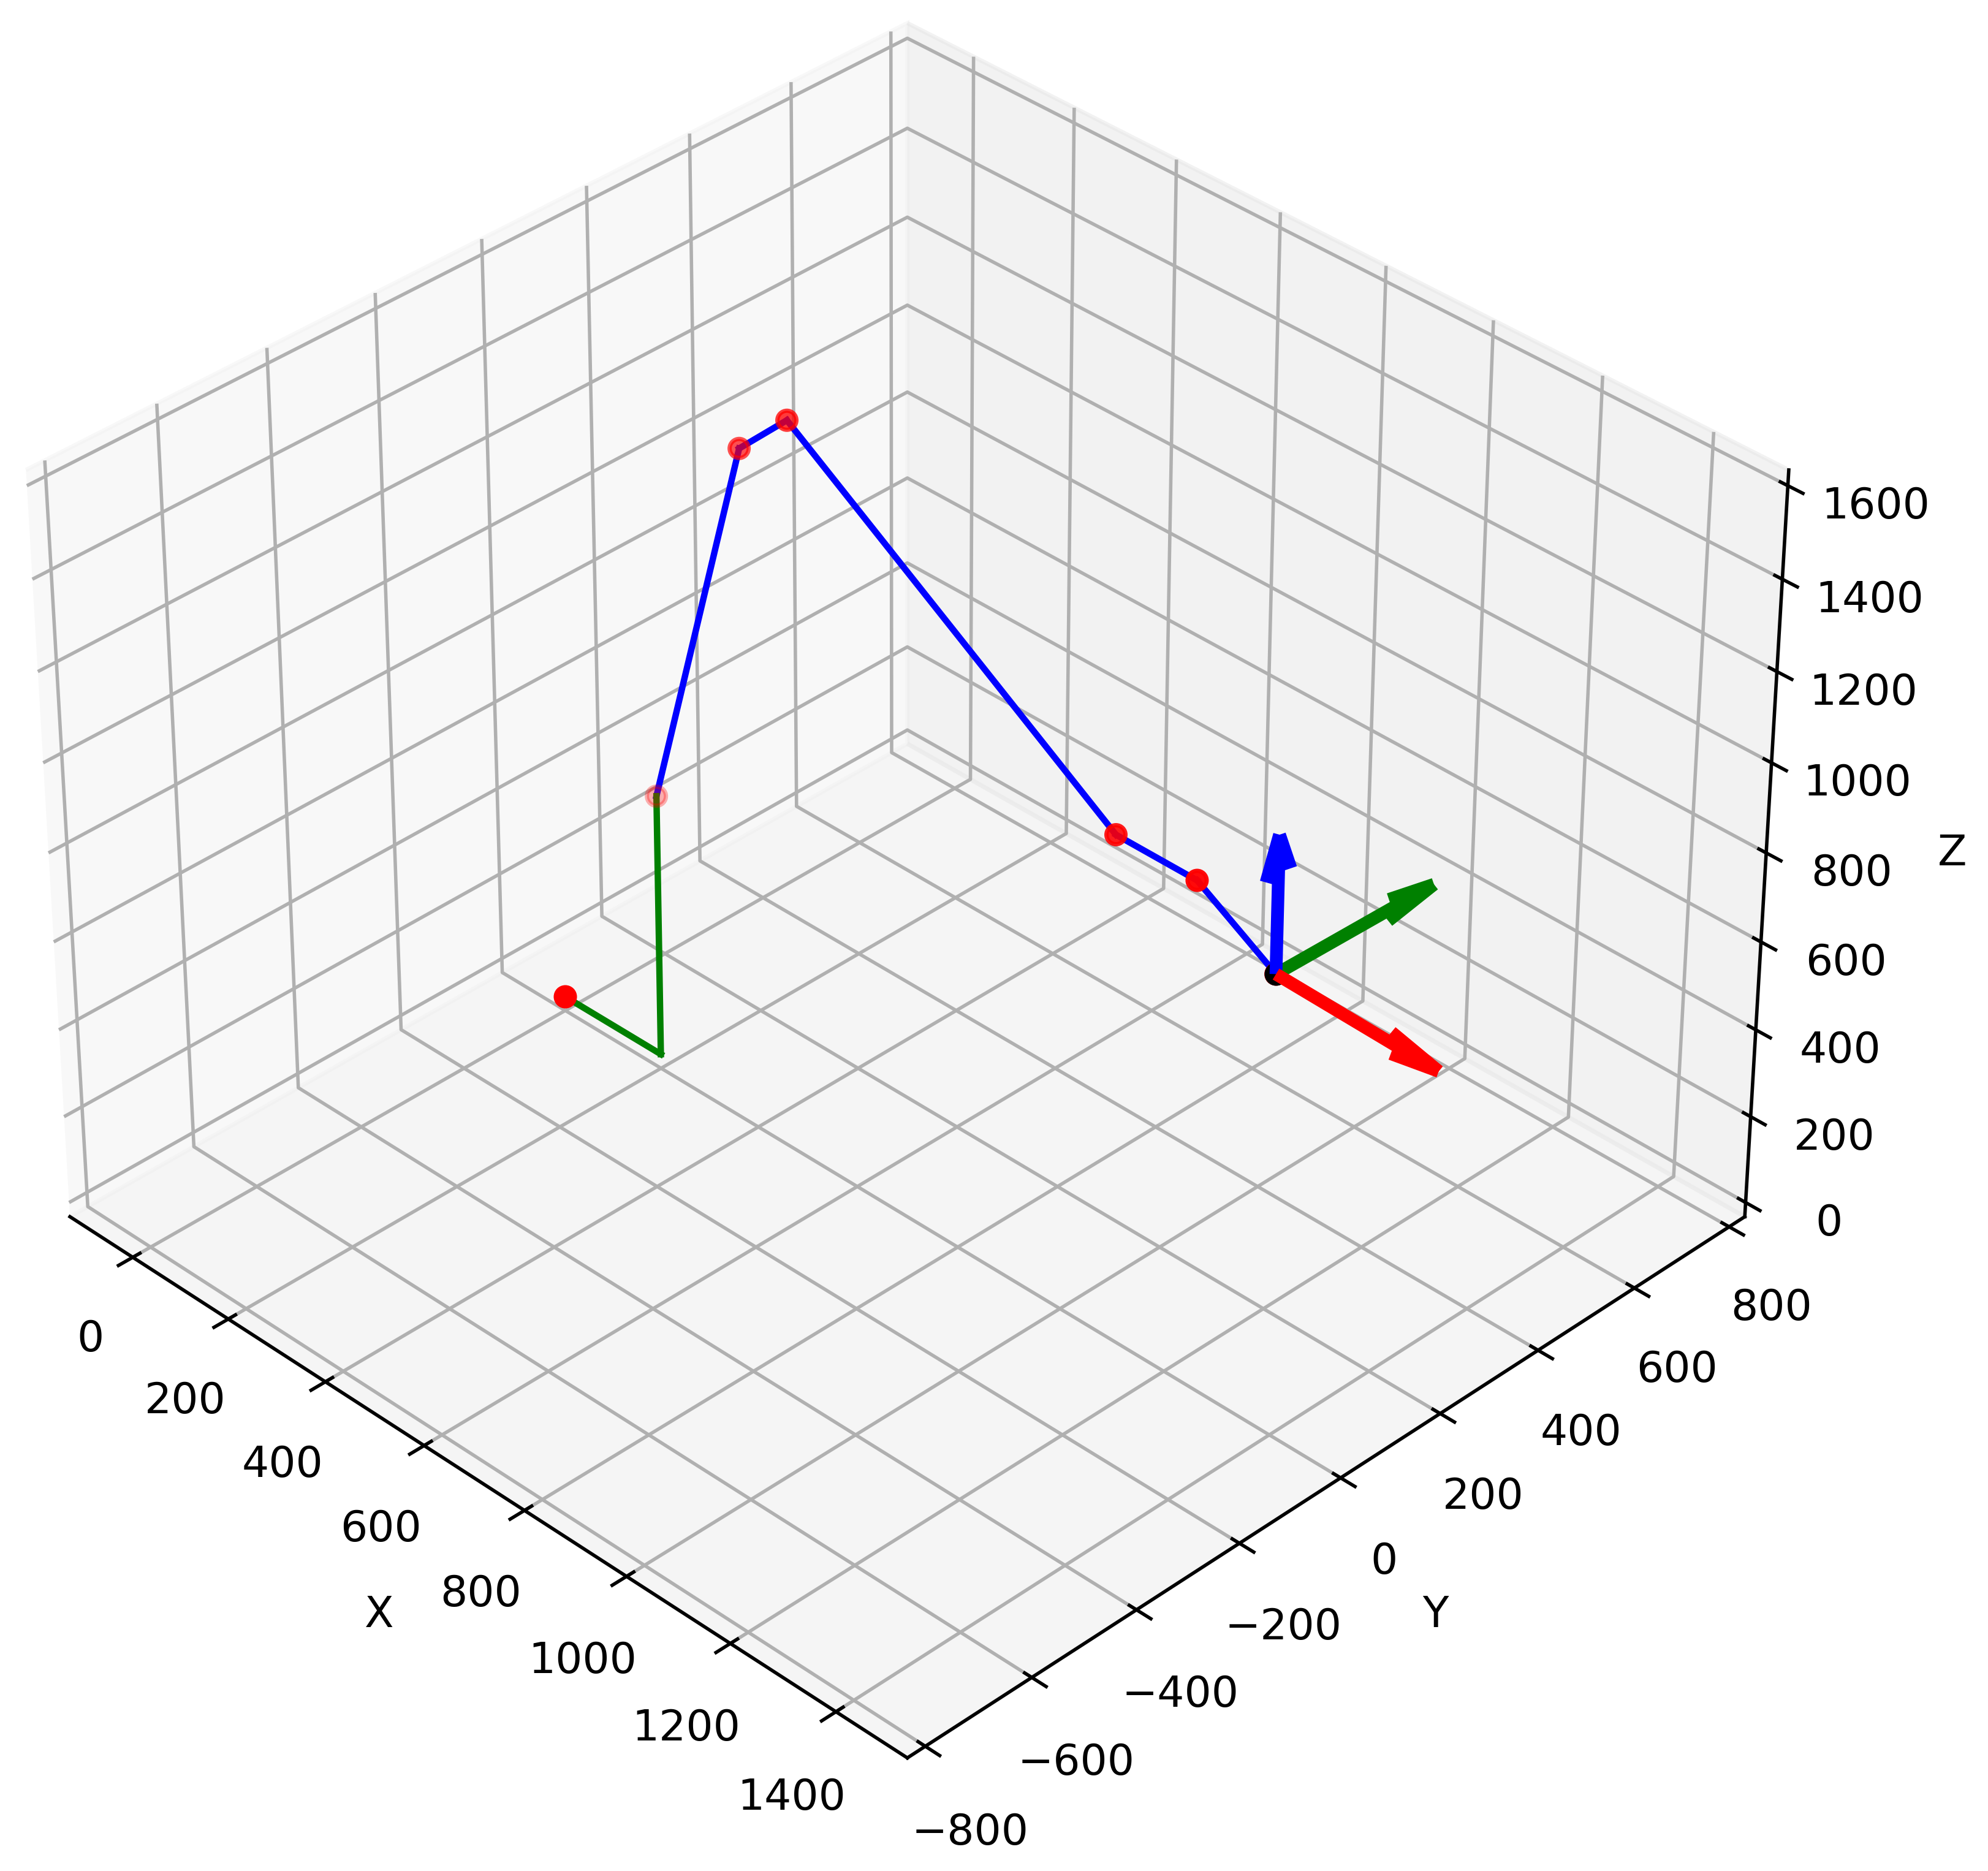
\includegraphics[width=0.9\textwidth]{figures/robotprog.png}}
	\caption{Visualization of the modeled robot}
	\label{robotprog}
\end{figure}


The arrows depicted in the figure represent the coordinate axes of the \acrshort{TCP}. For simplicity, the \acrshort{TCP} is considered to be the endpoint of the last joint. The X-axis is denoted in red, while the Y-axis and Z-axis are represented by the colors green and blue, respectively. The first link, originating from the point X=0, Y=0, Z=0, is displayed in green.

The schematic of the modeled robot can be observed in Figure \ref{schema}. In this specific configuration, all joints are in their initial position with no rotation applied.


\begin{figure}[H]
	\centerline{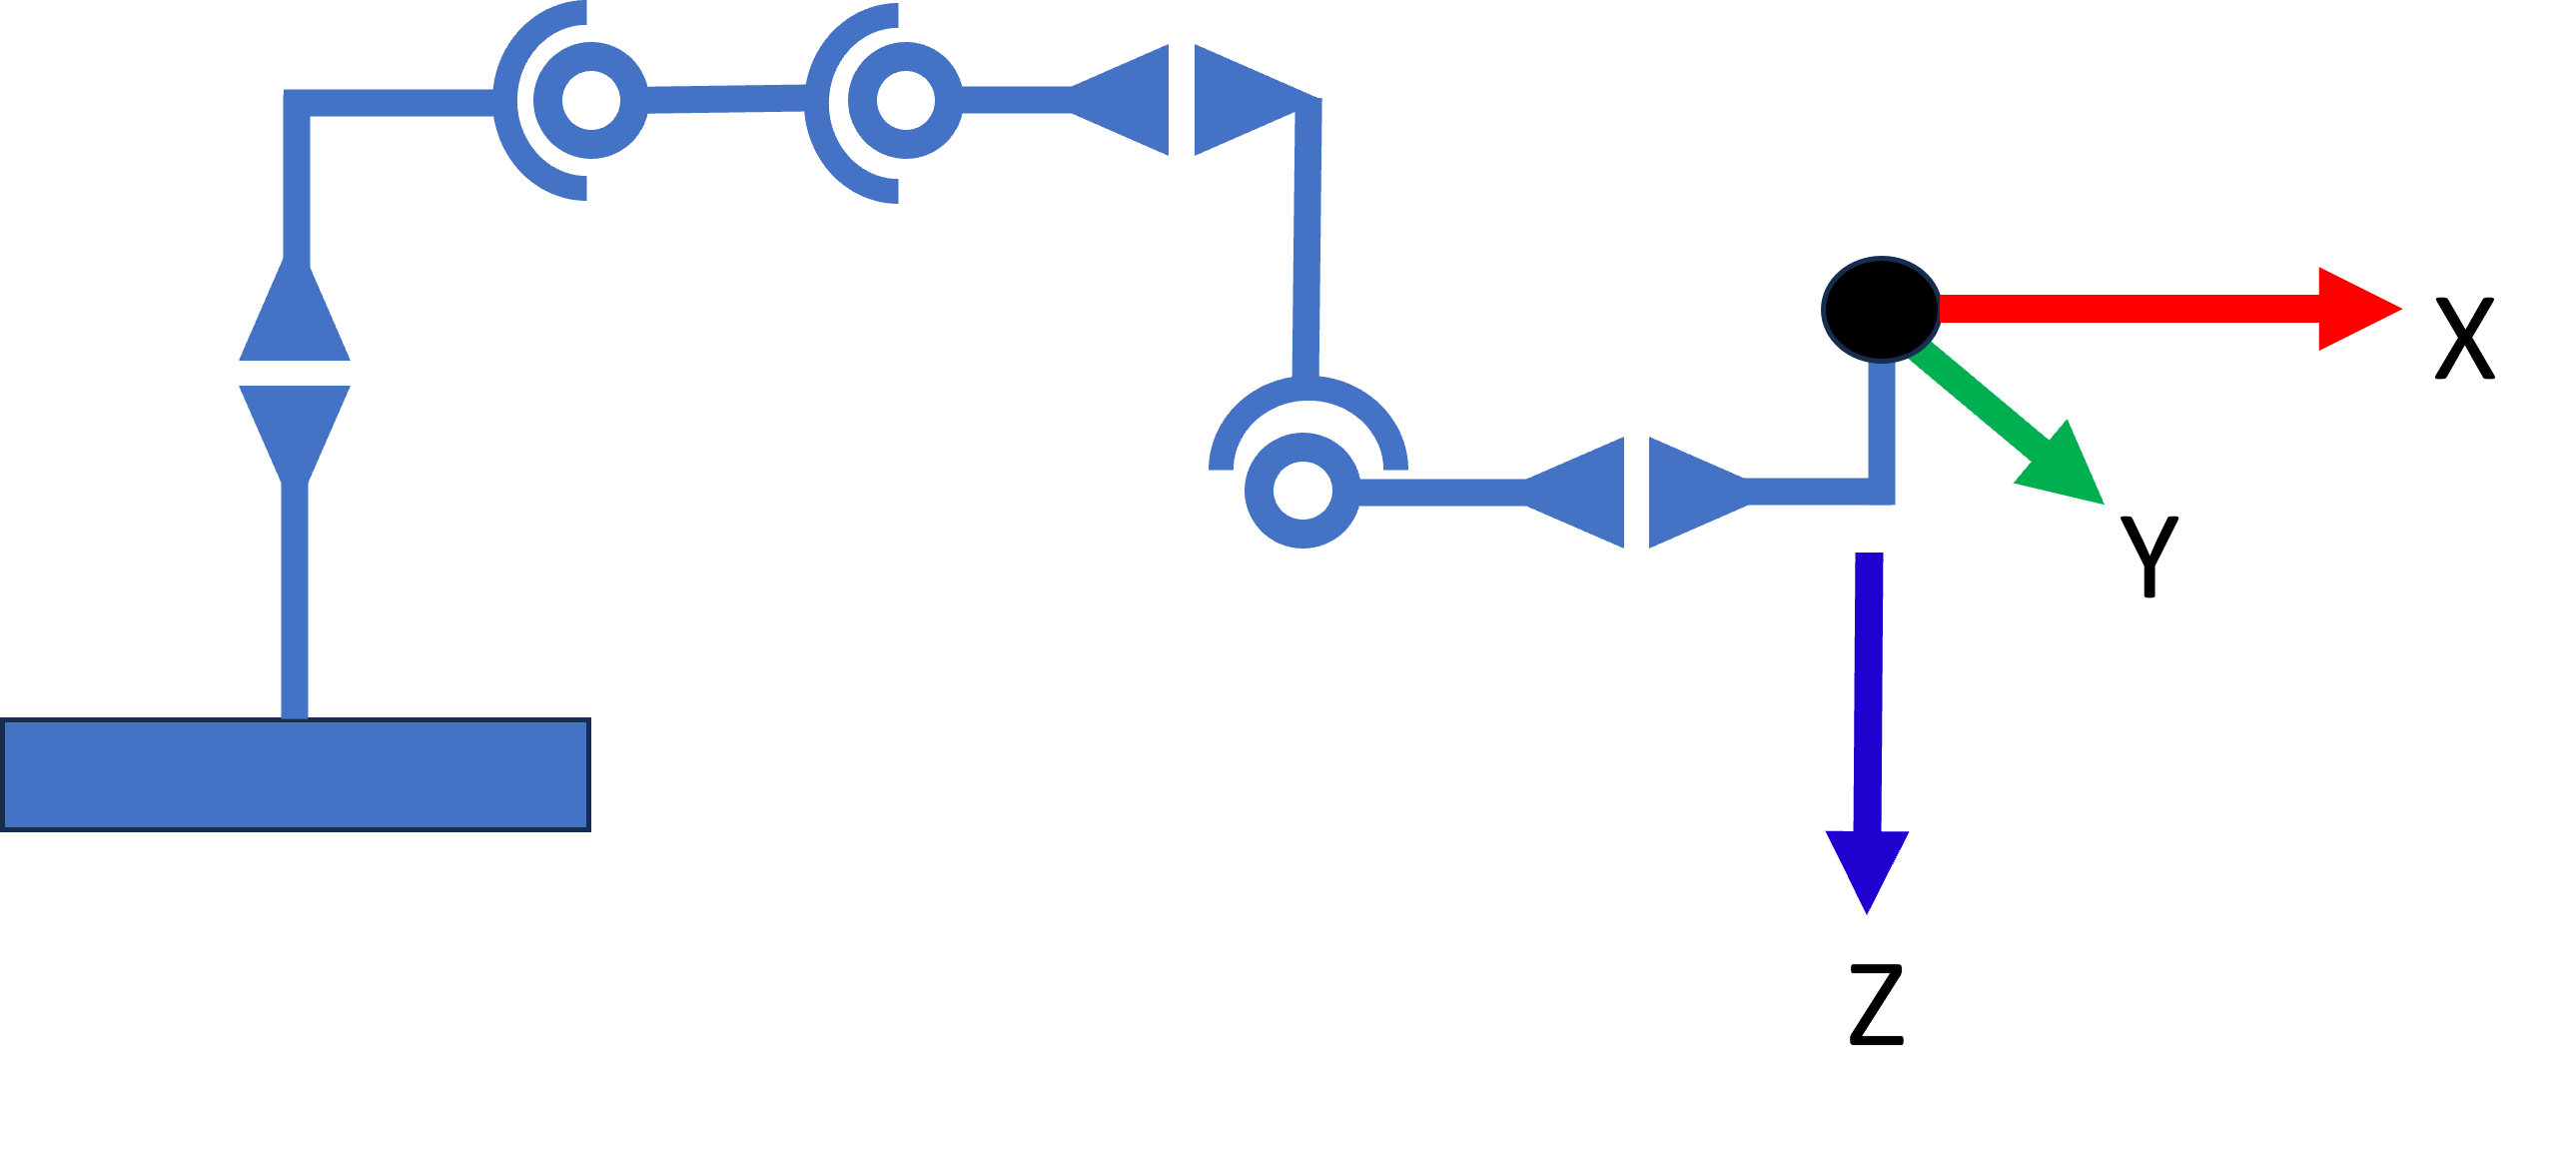
\includegraphics[width=0.7\textwidth]{figures/schema.png}}
	\caption{Schematics of the modeled robot}
	\label{schema}
\end{figure}

\subsection{Modeling a basic Toolpath}\label{MBT}
Before analyzing the process parameters, it is necessary to define a toolpath for the \acrshort{TCP} to follow. In this case, three options are presented, each consisting of 3000 coordinates. It should be noted that the redundant degree of freedom in these cases is the rotation around the Z-axis. This rotation will be adjusted to determine the optimal value for the desired outcome.

The first toolpath, depicted in Figure \ref{path1}, represents a converging-diverging spiral. Figure \ref{path2} illustrates a converging infinity-loop, and Figure \ref{path3} displays a forward-moving sinusoidal curve.

The corresponding equations for these toolpaths are given by Equation \ref{eq1}, Equation \ref{eq2}, and Equation \ref{eq3}. The variable \textit{iter} ranges from 0 to 3000 and is used to calculate the X, Y, and Z coordinates. Trigonometric functions are employed using the \textit{Numpy} library. Currently, no rotation (A, B, or C) has been defined. Only the coordinates are specified. Each toolpath has specific dimensions and characteristics. Toolpaths 1 and 2 are continuous, while toolpath 3 exhibits abrupt changes in direction. Only toolpath 1 possesses rotational symmetry.

\begin{equation}\label{eq1}
\begin{split}
x &= np.cos(np.deg2rad(iter)) * (500 - iter / 3)\\
y &= np.sin(np.deg2rad(iter)) * (500 - iter / 3)\\
z &= iter / 10
\end{split}
\end{equation}


\begin{equation}\label{eq2}
\begin{split}
x &= np.sin(np.deg2rad(iter)) * (400-iter / 5)\\
y &= np.sin(np.deg2rad(iter)) * np.cos(np.deg2rad(iter)) * (500-iter / 6)\\
z &= iter / 10
\end{split}
\end{equation}

\begin{equation}\label{eq3}
\begin{split}
x &= np.sin(np.deg2rad(iter)) * 200\\
y &= iter / 3 - (2500/6)\\
z &= np.sin(np.deg2rad(x))*100
\end{split}
\end{equation}


\begin{figure}[H]% [H] is so declass\'e!
	\centering
	\begin{minipage}{0.5\textwidth}
		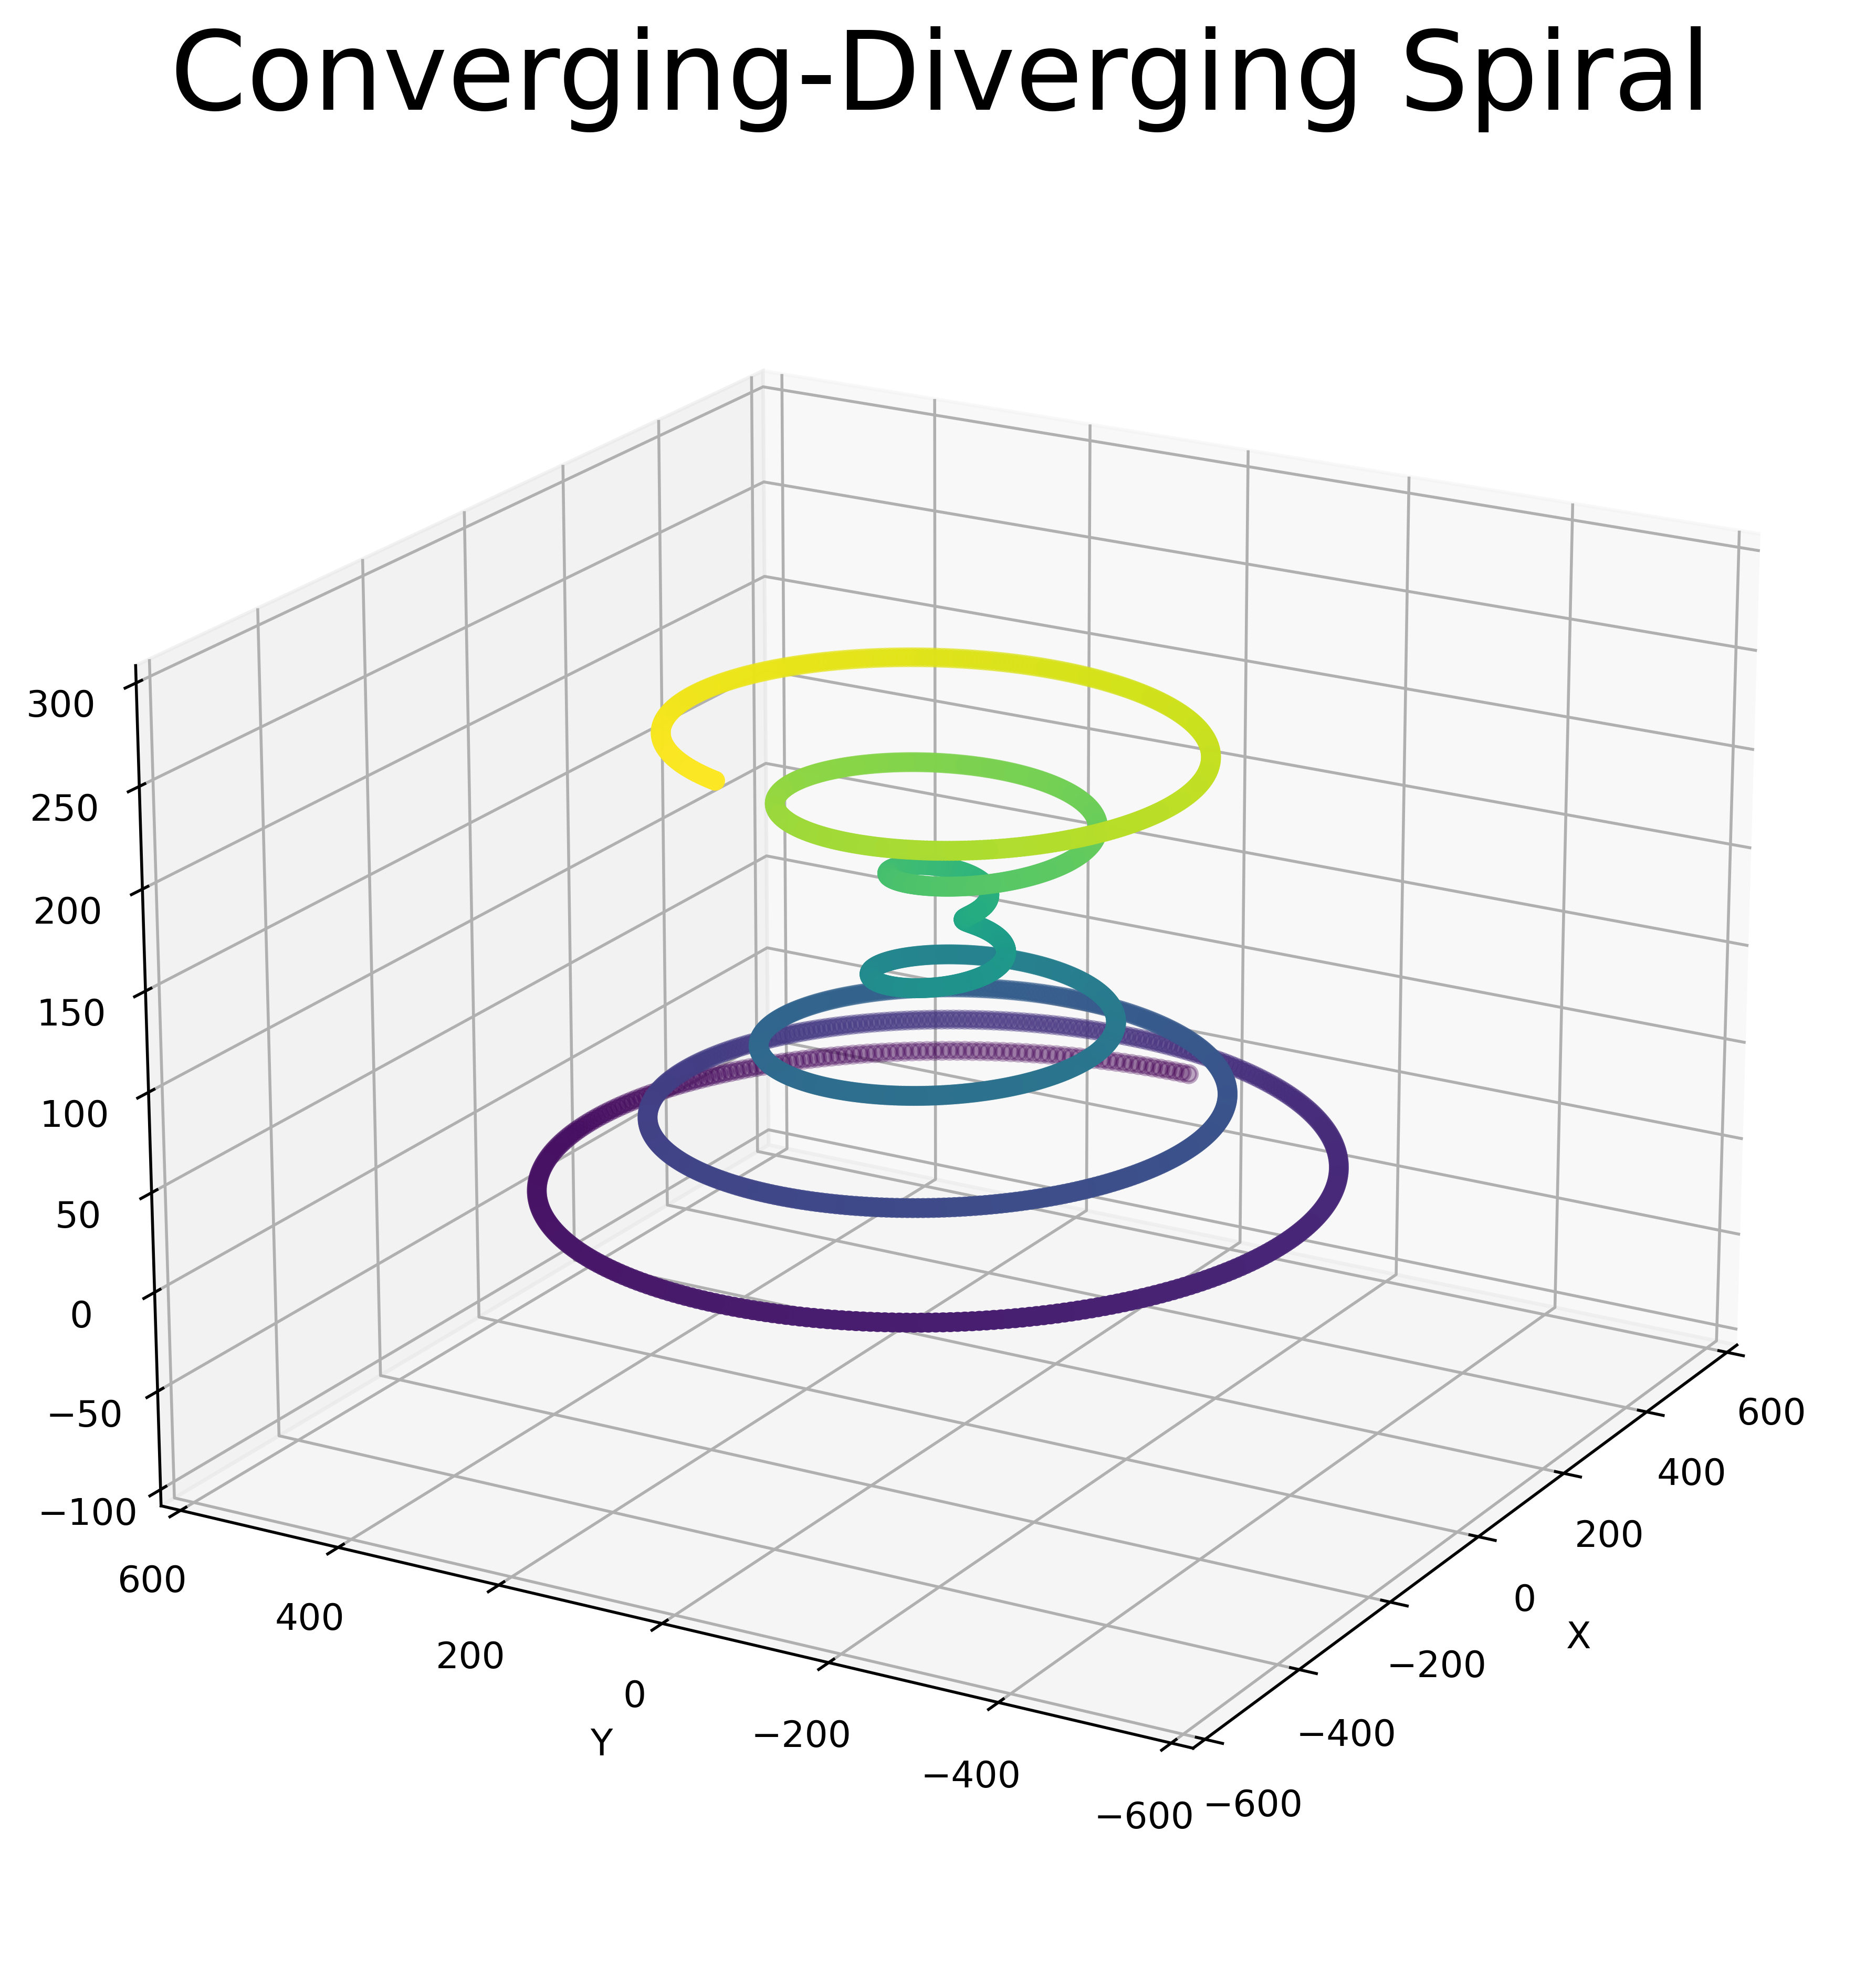
\includegraphics[width=\textwidth]{figures/path1.png}
		\caption{Toolpath 1: Converging-Diverging Spiral}
		\label{path1}
	\end{minipage}\hfill
	\begin{minipage}{0.5\textwidth}
		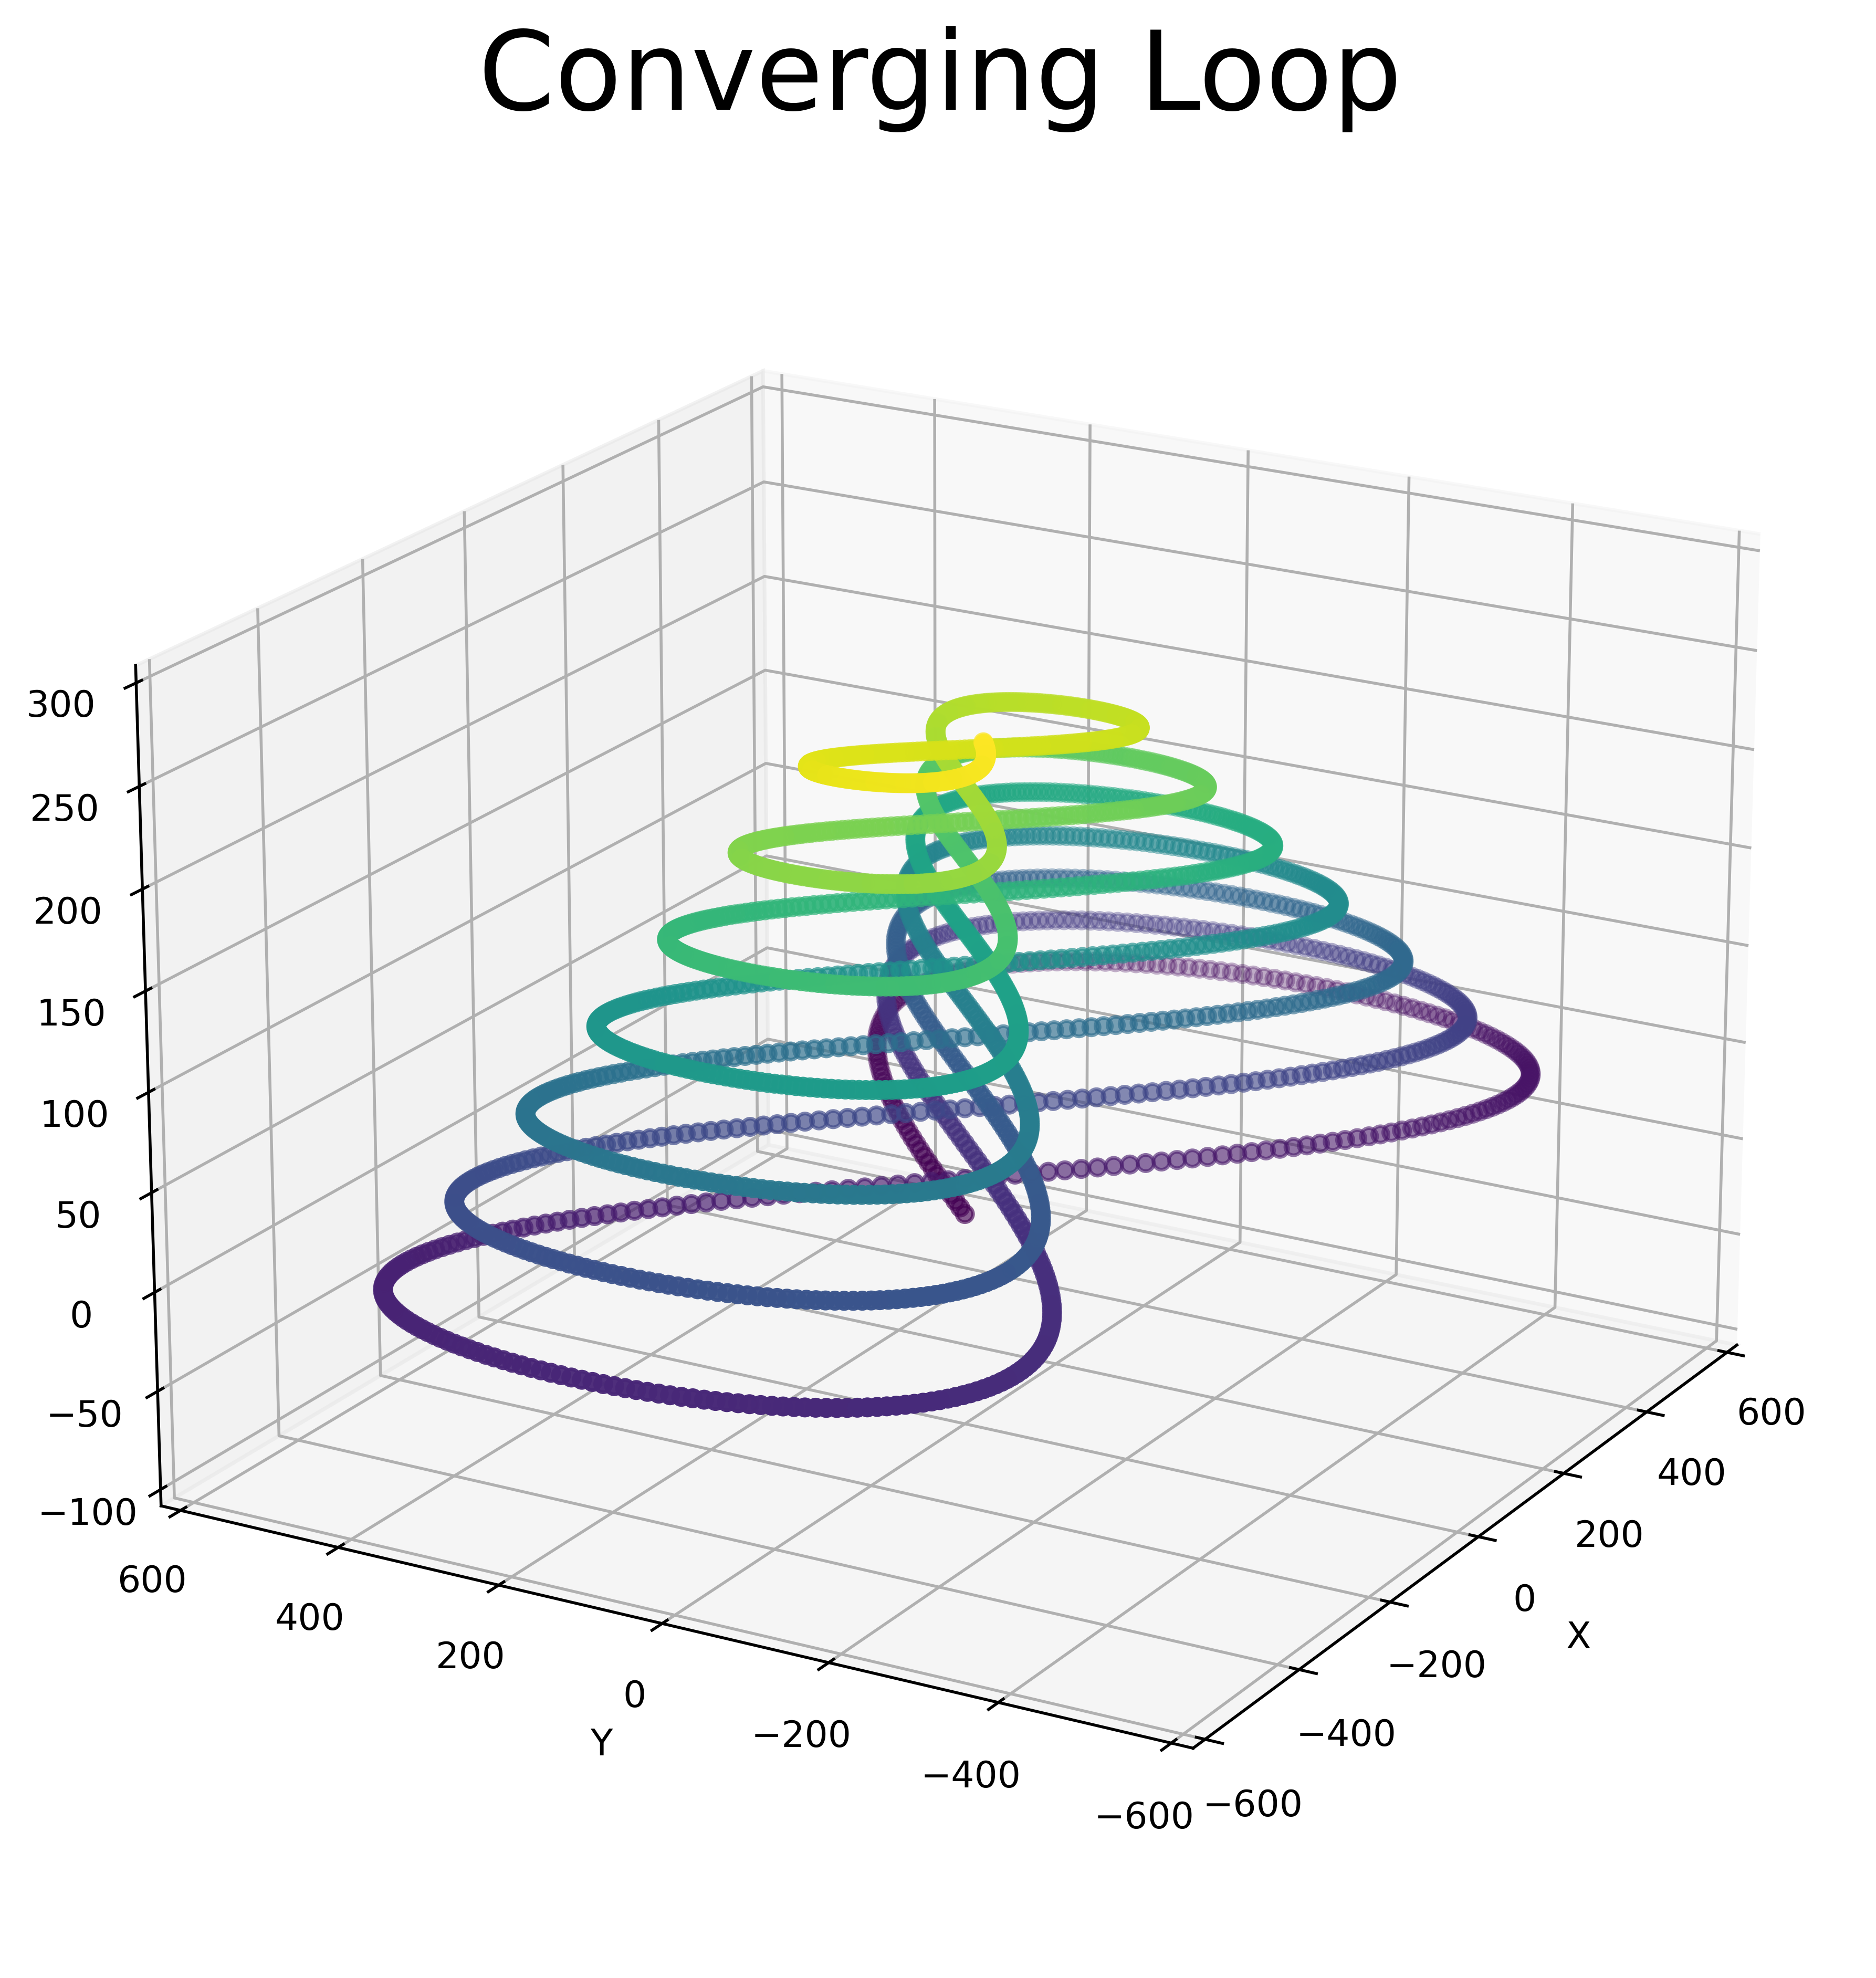
\includegraphics[width=\textwidth]{figures/path2.png}
		\caption{Toolpath 2: Converging Loop}
		\label{path2}
	\end{minipage}\par
	\vskip\floatsep% normal separation between figures
	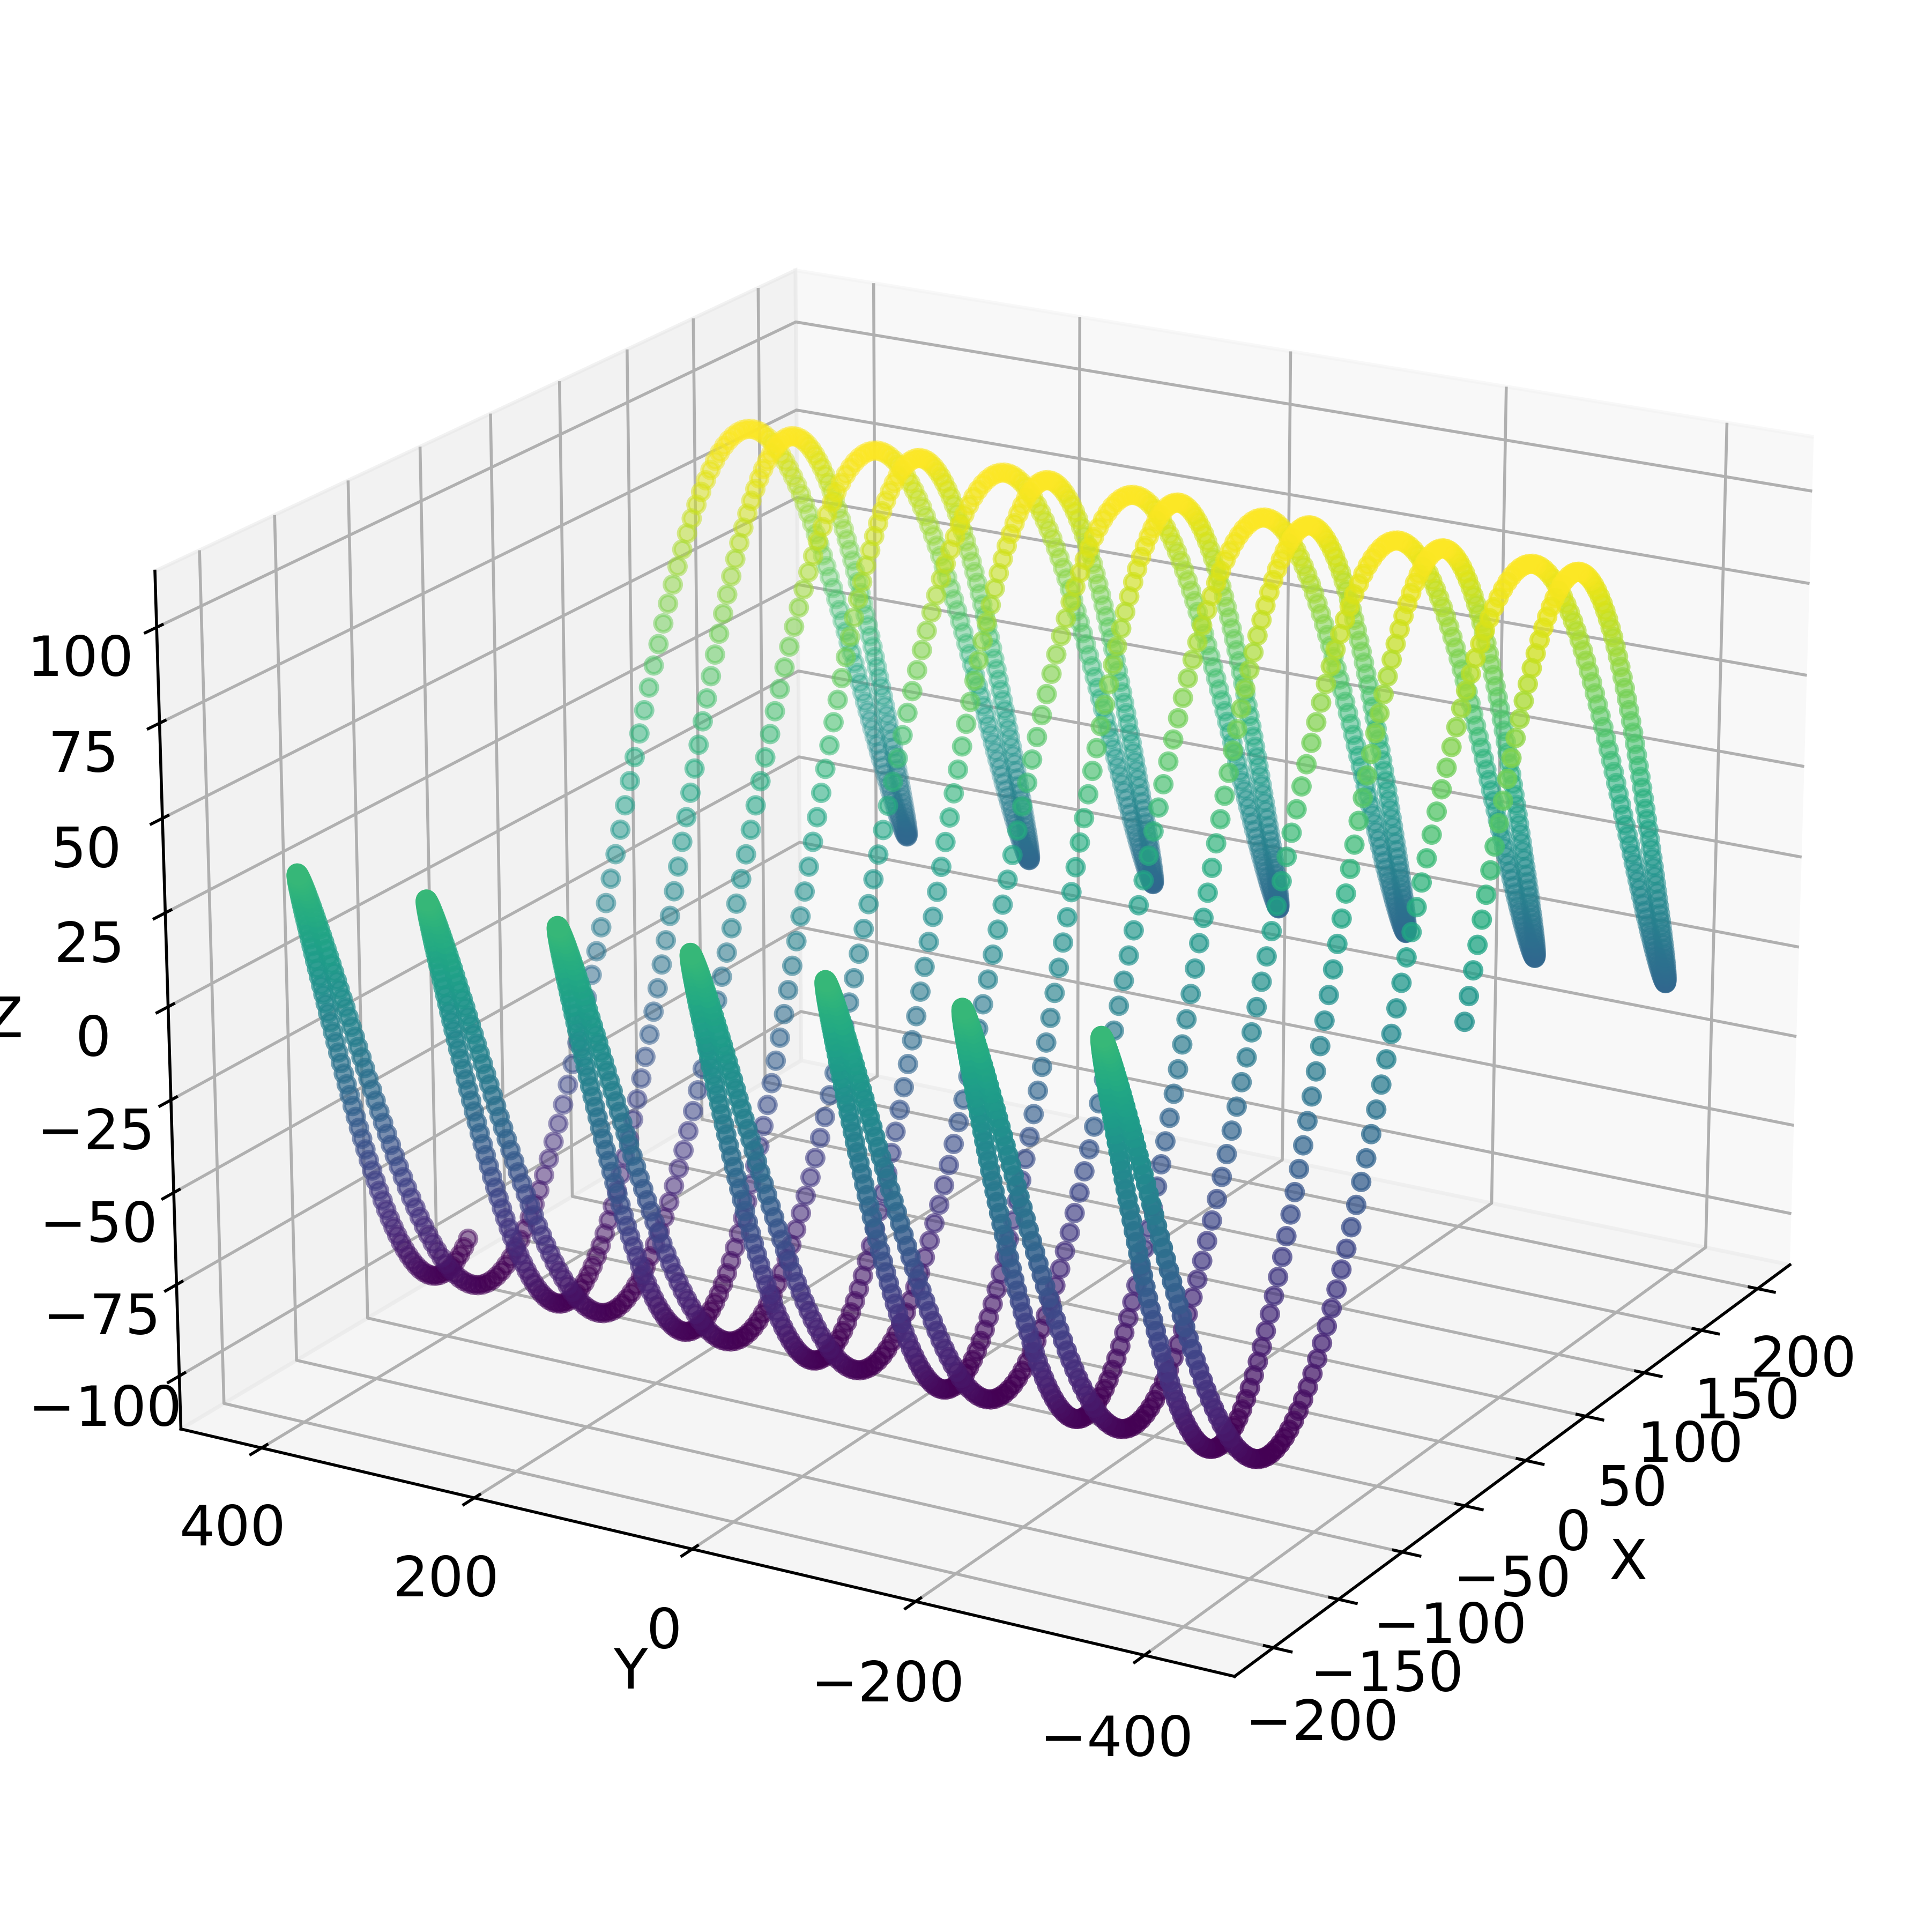
\includegraphics[width=0.5\textwidth]{figures/path3.png}

	\caption{Toolpath 3: Pendulum Oscillation}
	\label{path3}
\end{figure}

\newpage
Figure \ref{TP1robot} illustrates the robot and Toolpath 1 (defined by Equation \ref{eq1}) at the toolpath's final position. The origin of the toolpath is shifted by X=1000 and Z=600 relative to the robot's coordinate system. No rotations are applied around the X, Y, and Z axes, resulting in A, B, and C being zero. Thus, the coordinate axes of the toolpath are parallel to the axes of the robot's coordinate system.



\begin{figure}[H]
	\centerline{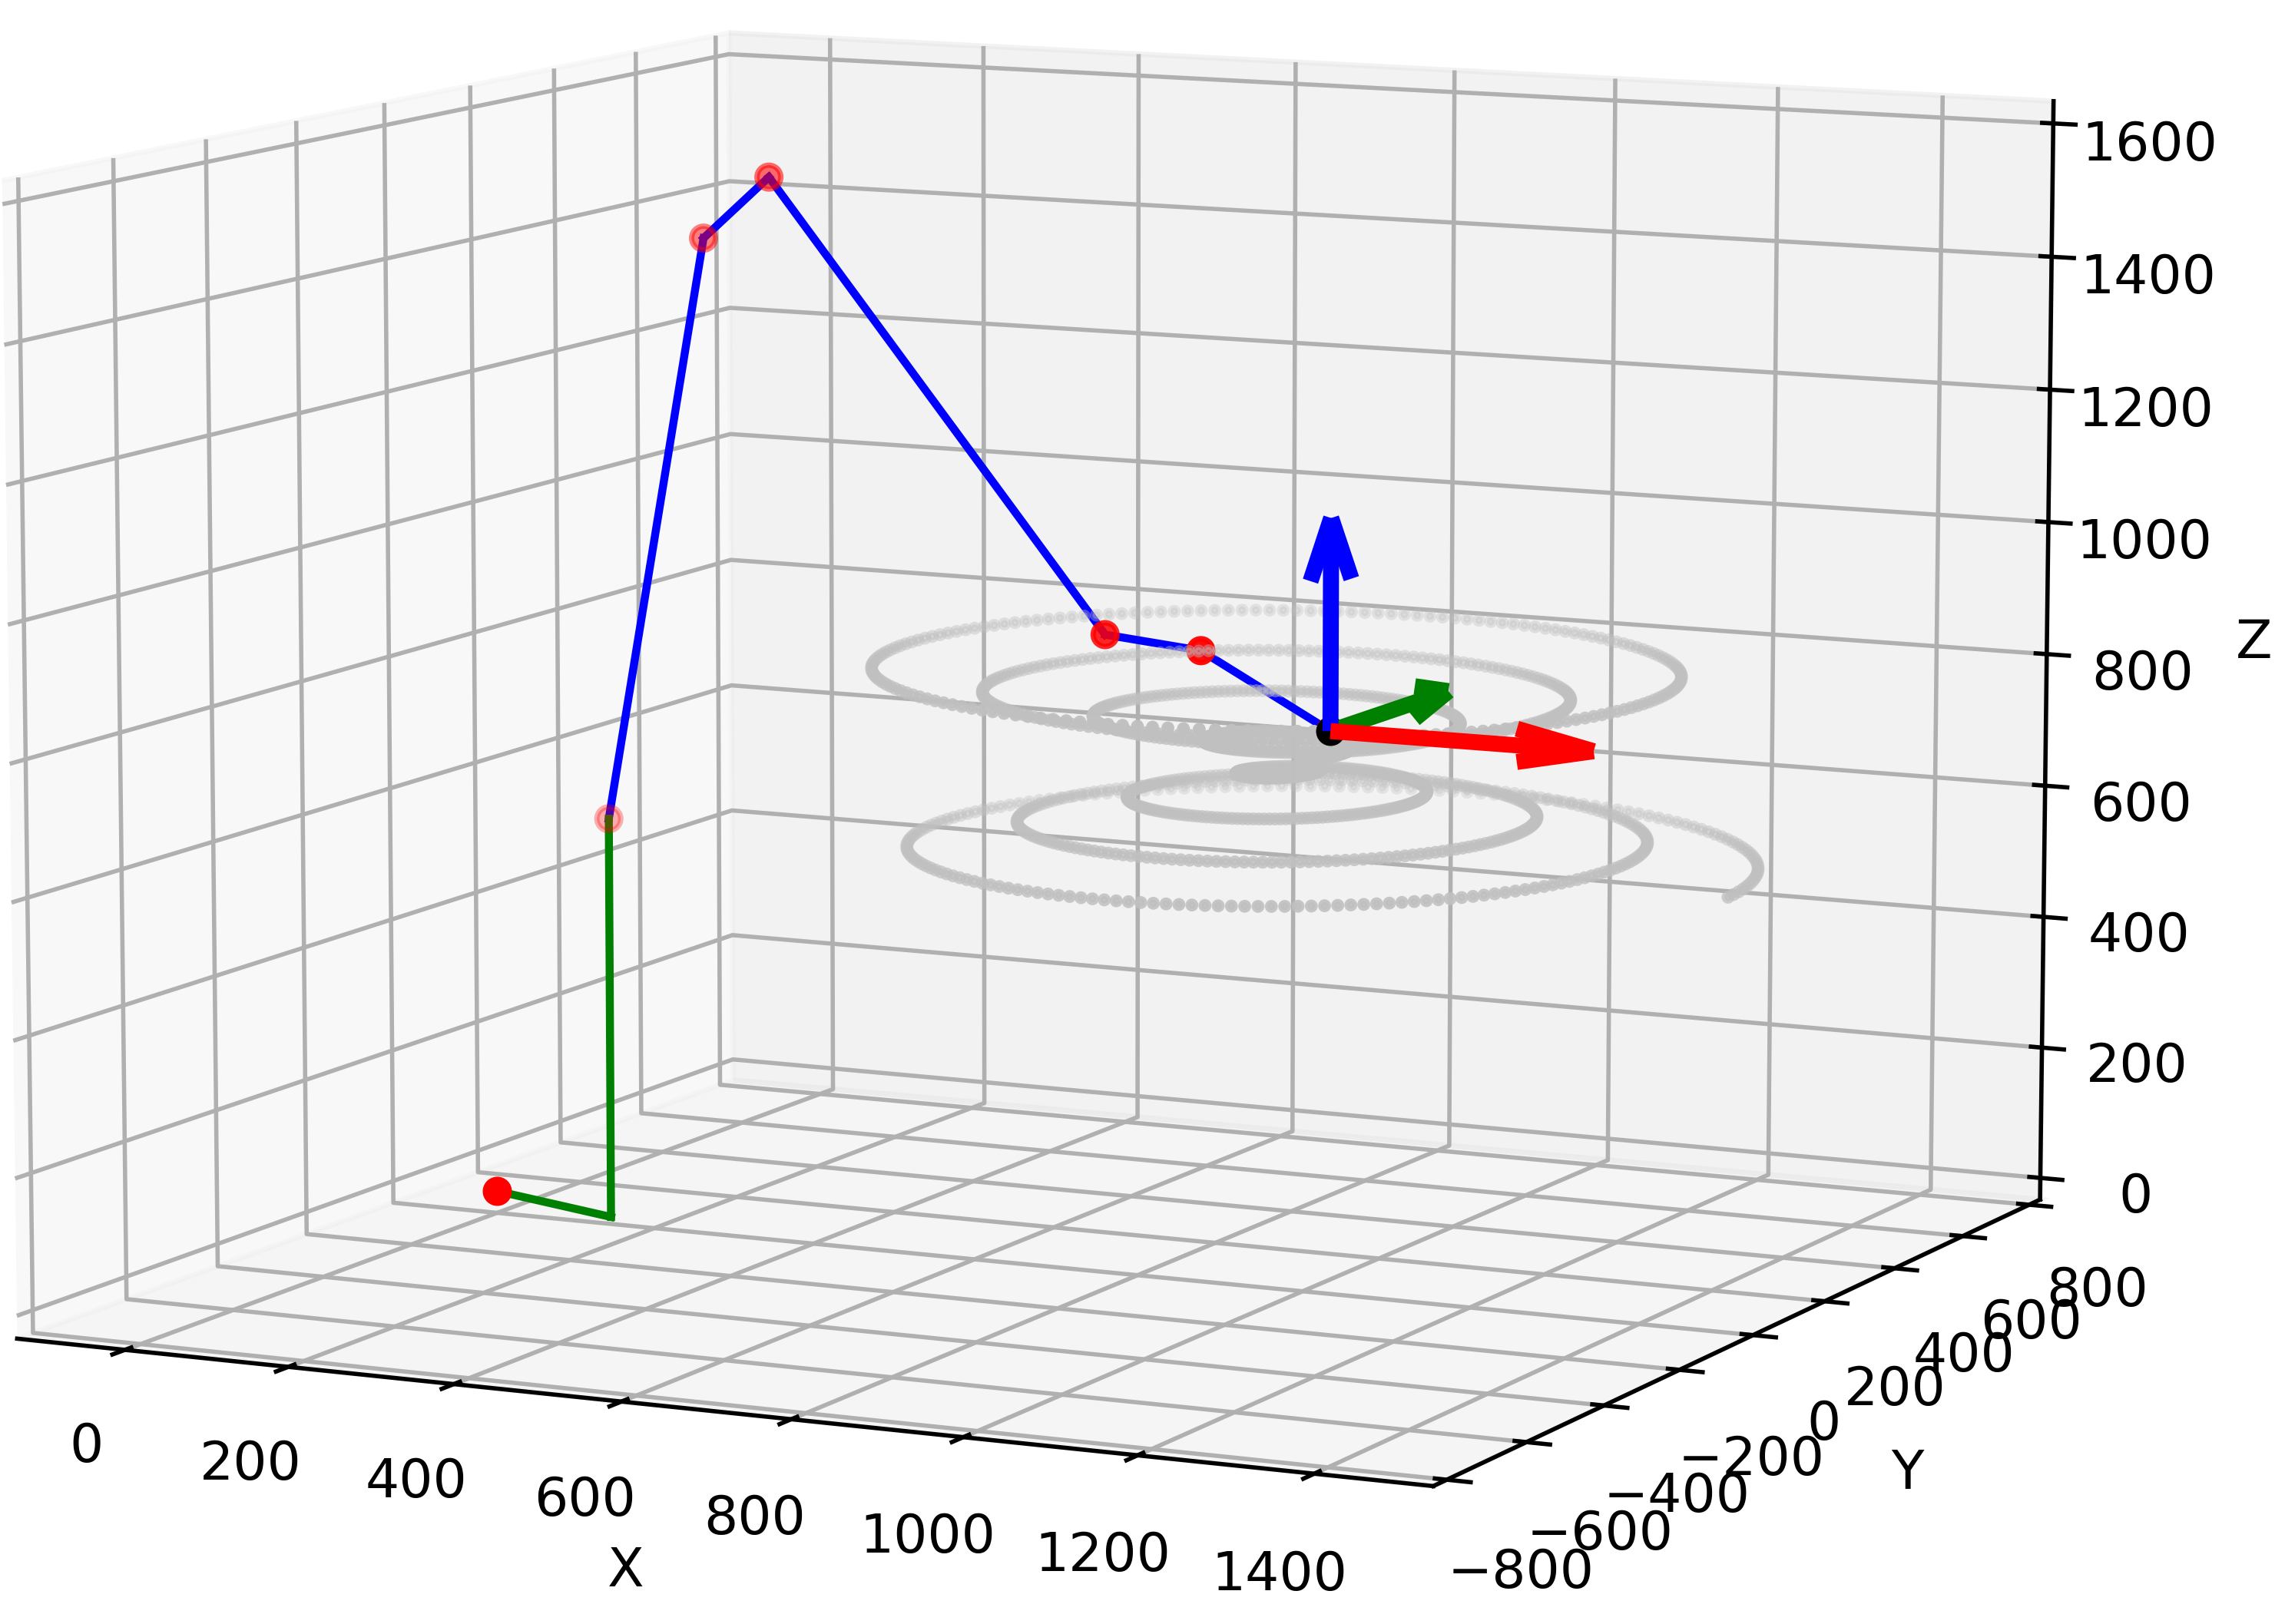
\includegraphics[width=0.9\textwidth]{figures/robotANDpath1.png}}
	\caption{Toolpath 1 with robot model}
	\label{TP1robot}
\end{figure}




\subsection{Extracting process parameters}
Using the inverse kinematics algorithm from the Python library \textit{visual\_kinematics}, the joint angles for each coordinate can be computed. To achieve this, the rotations A, B, and C need to be defined. The result is a time series that contains the corresponding joint positions. Currently, all coordinates must be traversed in equidistant time steps. With this information, it becomes possible to calculate the velocity and other related parameters. By transforming all the data from the time series into scalar values and calculating the local score, the global score can be determined.
\newpage
\section{Testing and Validation}%

\subsection{Toolpath Evaluation with one Redundant DoF}
%\subsubsection{Obtaining Joint Positions}
As discussed in Chapter \ref{MBT}, the toolpath remains constant with respect to the X-Y-Z coordinates. The fixed boundary conditions for the robot are that there are no rotations around the X and Y axes, resulting in A and B both being equal to zero. The user has the ability to set the degree of freedom for the rotation around the Z-axis, which is the redundant degree of freedom. Figure \ref{TP1ABC0} displays the variation of each joint over time for toolpath 1. In this specific case, the rotations A, B, and C are all set to 0. The entire toolpath is traversed in 300 seconds.

\begin{figure}[H]
	\centerline{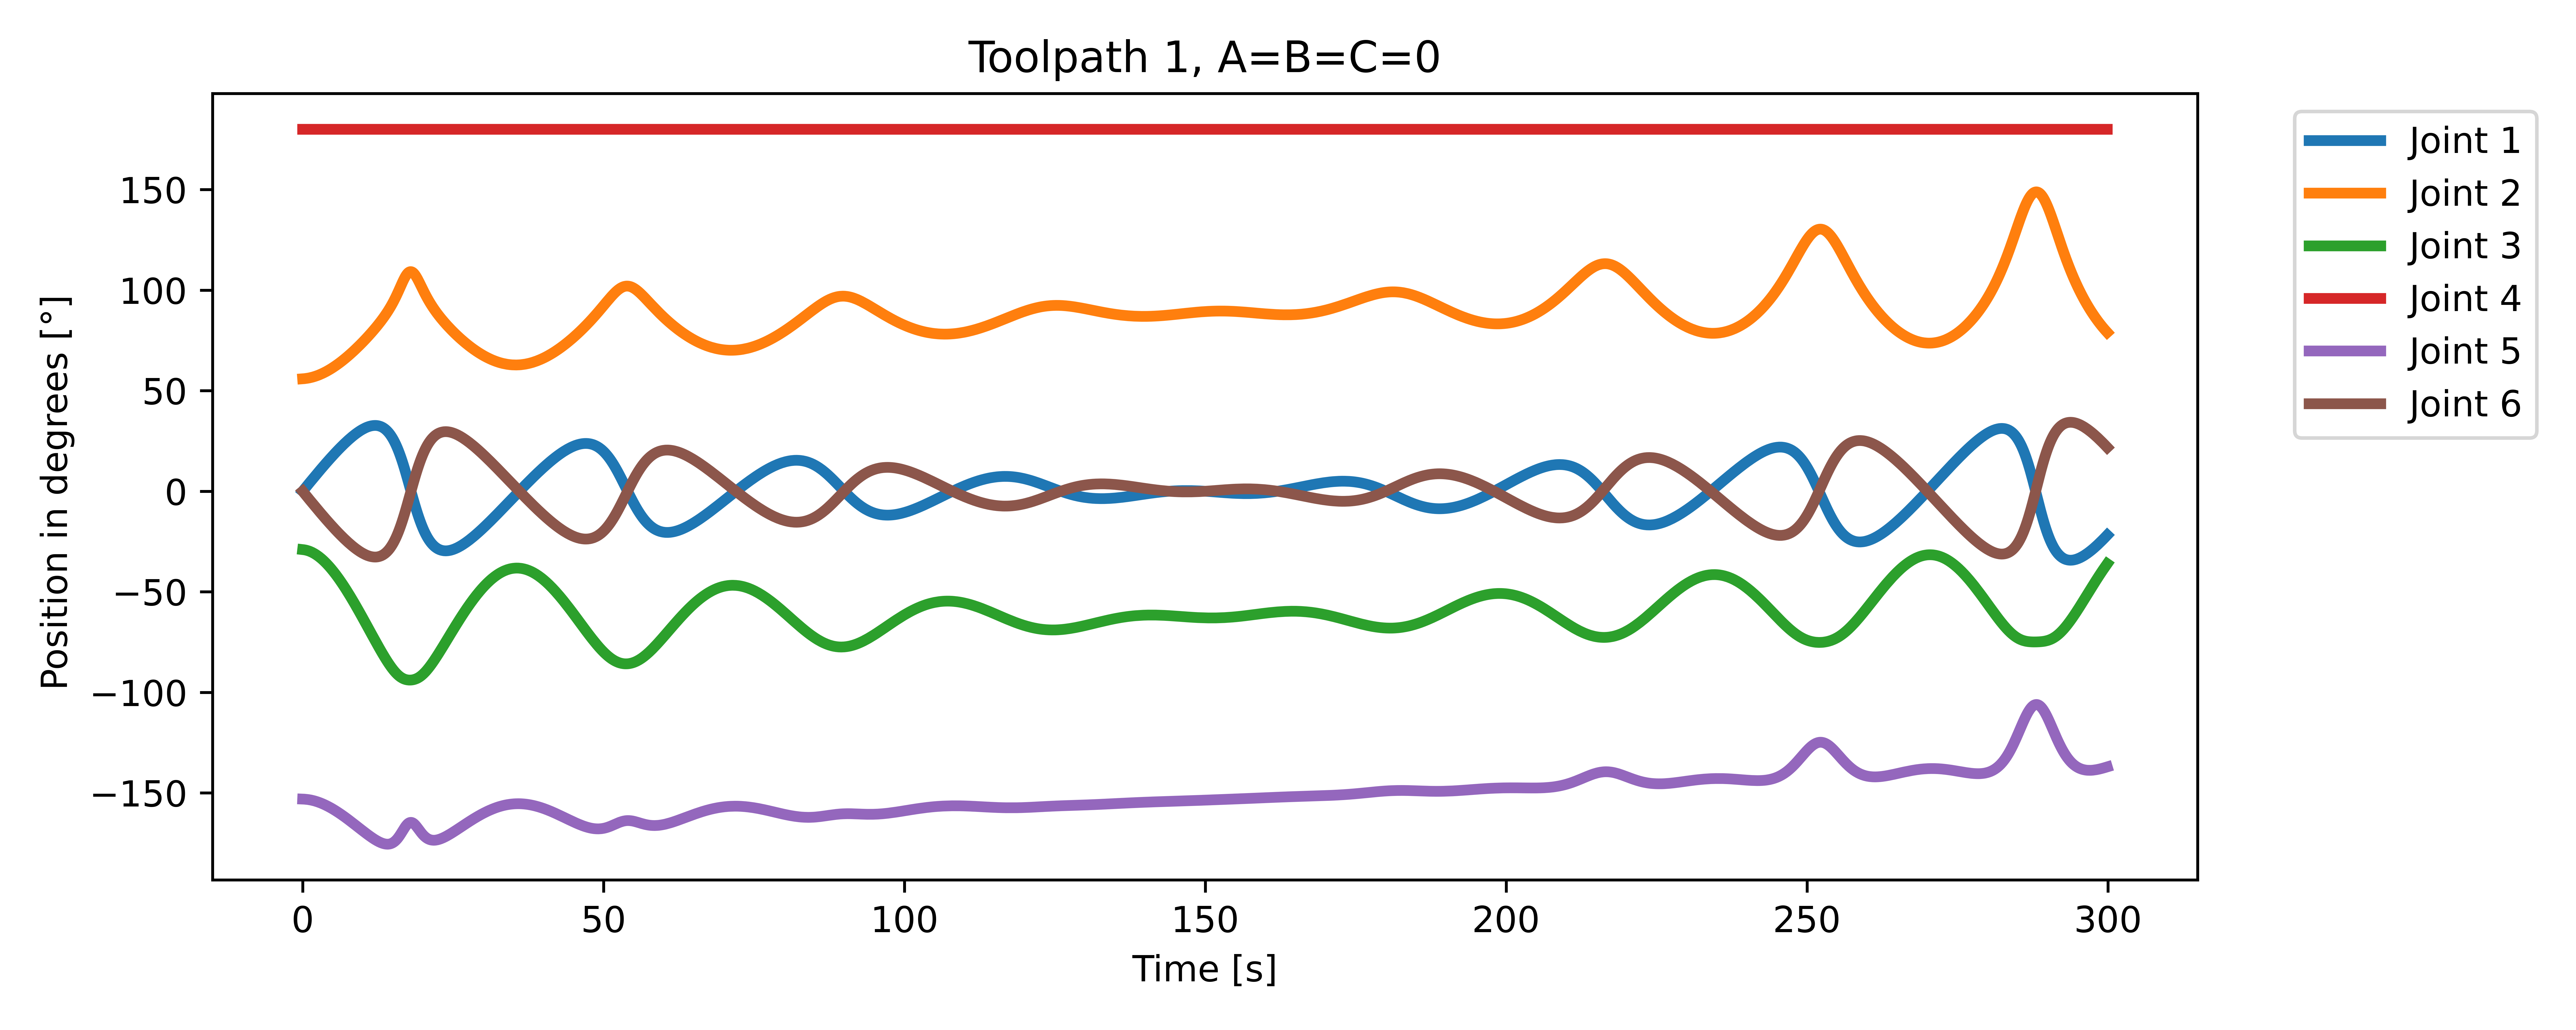
\includegraphics[width=1\textwidth]{figures/TP1ABC0.png}}
	\caption{Visualization of the joint positions over time for toolpath 1 with C=0}
	\label{TP1ABC0}
\end{figure}

Figure \ref{TP1ABC45} depicts the joint positions over time for the toolpath with a 45° rotation around the Z-axis (C = 45°). It is noticeable that joint 4 and joint 5 have undergone changes in their respective ranges. Furthermore, joint 6 exhibits a significantly larger amplitude towards the end of the toolpath, in comparison to the case with no rotation (C=0).

\begin{figure}[H]
	\centerline{\includegraphics[width=1\textwidth]{figures/TP1ABC45.png}}
	\caption{Visualization of the joint positions over time for toolpath 1 with C=45°}
	\label{TP1ABC45}
\end{figure}


%Joints 1 and 6 oscillate out of phase relative to each other around a zero degrees. Joint 3 remains constantly at 180 degrees. Joint 2 and 5 also oscillate and slightly increase.

Figure \ref{TP1ABC0} illustrates the variations in each joint over time for toolpath 2 (Eq. \ref{eq2}) without any rotation. Unlike toolpath 1, the amplitudes notably decrease towards the end of the toolpath. This observation aligns with the unique characteristics of different toolpaths.
 
 %In this case all joints show a oscillation except joint 4.
\begin{figure}[H]
	\centerline{\includegraphics[width=1\textwidth]{figures/TP2ABC0.png}}
	\caption{Visualization of the joint positions over time for toolpath 2}
	\label{TP2ABC0}
\end{figure}

%ToDo: EXPLAIN WHY JOINT 4 IS AT 180 all the time!!!!!!!!\newline
%\subsubsection{Selecting Process Parameters}
The next step involves selecting the process parameters of interest and assigning weights to each parameter. For that, a basic case is discussed. The selected process parameters are listed in table \ref{PPbasic}. The total number of direction changes in all joints and the total distance traveled are chosen due to their ease of implementation.

The number of direction changes is assigned an importance factor of 0.2.
The total travel in all joints is combined and is given an importance factor of 0.4.
Additionally, the acceleration of joint 1 is analyzed. To obtain a scalar value for the acceleration, the individual acceleration values are squared and then summed up. The importance factor for acceleration is 0.4.
Velocity, acceleration, and jerk are disregarded for all other joints.

\begin{table}[H]
	\centering
	\begin{tabular}{||l|l||}
		Process parameters& Importance Factor \\
		\hline
		\hline
		\hline
		Direction changes in joints 1-6	&		0.2 \\
		Total travel in joints 1-6	&  	0.4 \\
		Acceleration in joint 1	& 		0.4\\
		
		\hline
		\hline
	\end{tabular}
	
	\caption{Selected process parameters and their importance factors}
	\label{PPbasic}
\end{table}


Since only one degree of freedom is being analyzed, it is possible to represent the individual local scores and global score as a one-dimensional graph. Firstly, toolpath 1 is analyzed by incrementing the redundant degree of freedom by 5 degrees, starting from -135 degrees and ending at 135 degrees.

Figure \ref{TP1-25} illustrates a case with a -45-degree rotation around the Z-axis for toolpath~1.
Similarly, Figure \ref{TP1+25} displays a case with a +45-degree rotation around the Z-axis for toolpath~1.

\begin{figure}[H]
	\centering
	\begin{minipage}{0.5\textwidth}
		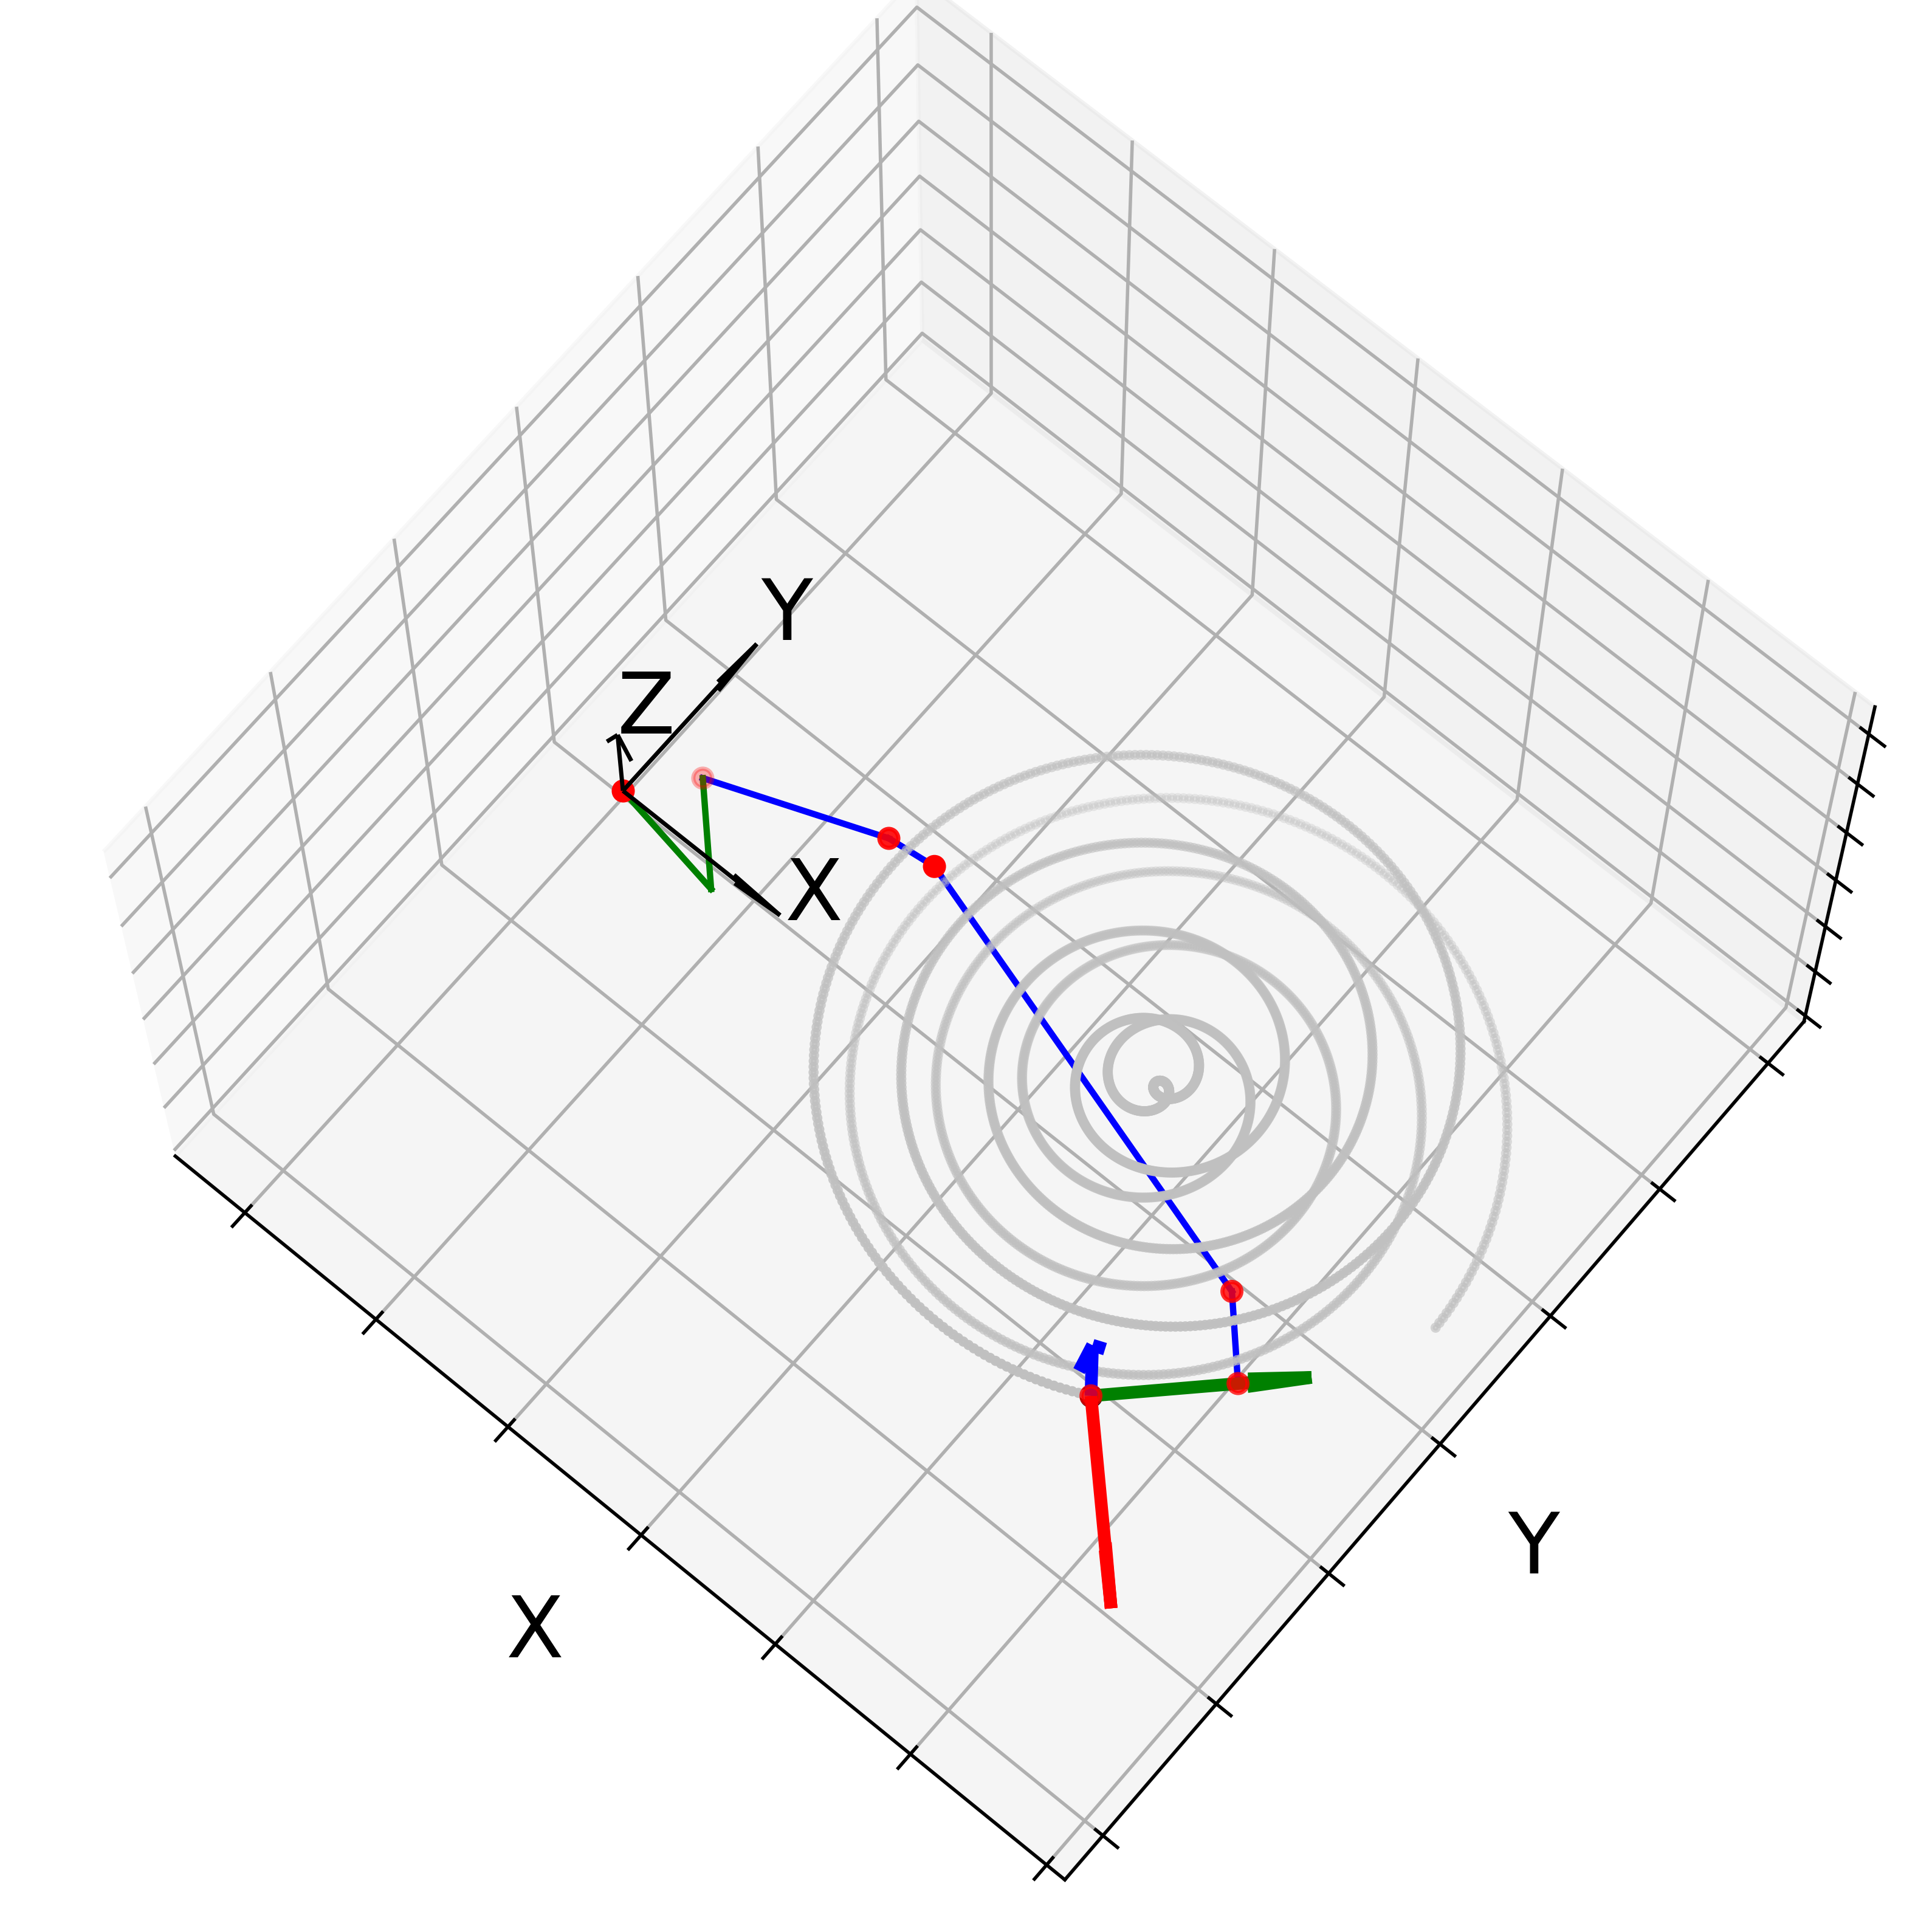
\includegraphics[width=\textwidth]{figures/robotANDpath1_-45.png}
		\caption{Toolpath 1 with A=0, B=0 and C = -45°}
		\label{TP1-25}
	\end{minipage}\hfill
	\begin{minipage}{0.5\textwidth}
		\includegraphics[width=\textwidth]{figures/robotANDpath1_45.png}
		\caption{Toolpath 1 with A=0, B=0 and C = 45}
		\label{TP1+25}
	\end{minipage}\par
\end{figure}

A total of 55 time series of joint positions are generated. On average, the inverse kinematics algorithm takes 35 seconds to calculate the joint values for all 3000 coordinates.

The process parameters are extracted and scaled in relation to each other, as described in Chapter~\ref{LRC}. It is important to note that before scaling, the selected process parameters are pre-multiplied by -1, as each process parameter should be minimized.

The arrays of local ratings are then multiplied by the weights selected in table \ref{PPbasic}.
Subsequently, the local scores of each process parameter can be plotted as a one-dimensional graph, as shown in figure \ref{LS1}. %It can be seen that the local scores of the selected process parameters have a significant variation in the range from -15 to 10 degrees.



\begin{figure}[H]
	\centerline{
\includegraphics[width=1\textwidth]{figures/LocalScores_1.png}}
	\caption{Local scores of each process parameter for toolpath 1}
	\label{LS1}
\end{figure}

The acceleration in joint 1 and the combined total travel in the joints exhibit a smooth oscillating curve with a decreasing amplitude towards the positive end of the analyzed range. It is worth mentioning that the maximum value that the local score can reach is 40 for acceleration and total travel, while for direction changes, the maximum score is 20. This is due to the assigned importance factors. The direction changes display a less smooth trajectory.

Next, the local scores are summed up to calculate the global score. The resulting array, displayed in figure \ref{GS1}, represents the global score achieved by varying the rotation around the Z-axis in relation to all other analyzed values. The green cross on the graph indicates the maximum attainable score and its corresponding rotation, compared to all analyzed boundary conditions.

\begin{figure}[H]
	\centerline{\includegraphics[width=1\textwidth]{figures/best_c_1.png}}
	\caption{Global score for toolpath 1}
	\label{GS1}
\end{figure}
In this particular case, the highest achievable score is 92.81 at -135 degrees. This nearly perfect score indicates that setting the rotation to -135 degrees results in minimal direction changes, minimal total travel, and close to minimal acceleration in joint~1. It is crucial to emphasize that this rating is only in comparison to the other analyzed boundary conditions.


The same analysis, using identical process parameters and weights, can be performed with toolpath 2 and toolpath 3. Figure \ref{TP2_combi} and figure \ref{TP3_combi} display the global and local scores for each analyzed value of the redundant degree of freedom. For toolpath 2, the best score is 93.4 at -115.0 degrees, while for toolpath 3, the best score is 88 at -80 degrees.

\begin{figure}[H]
\centerline{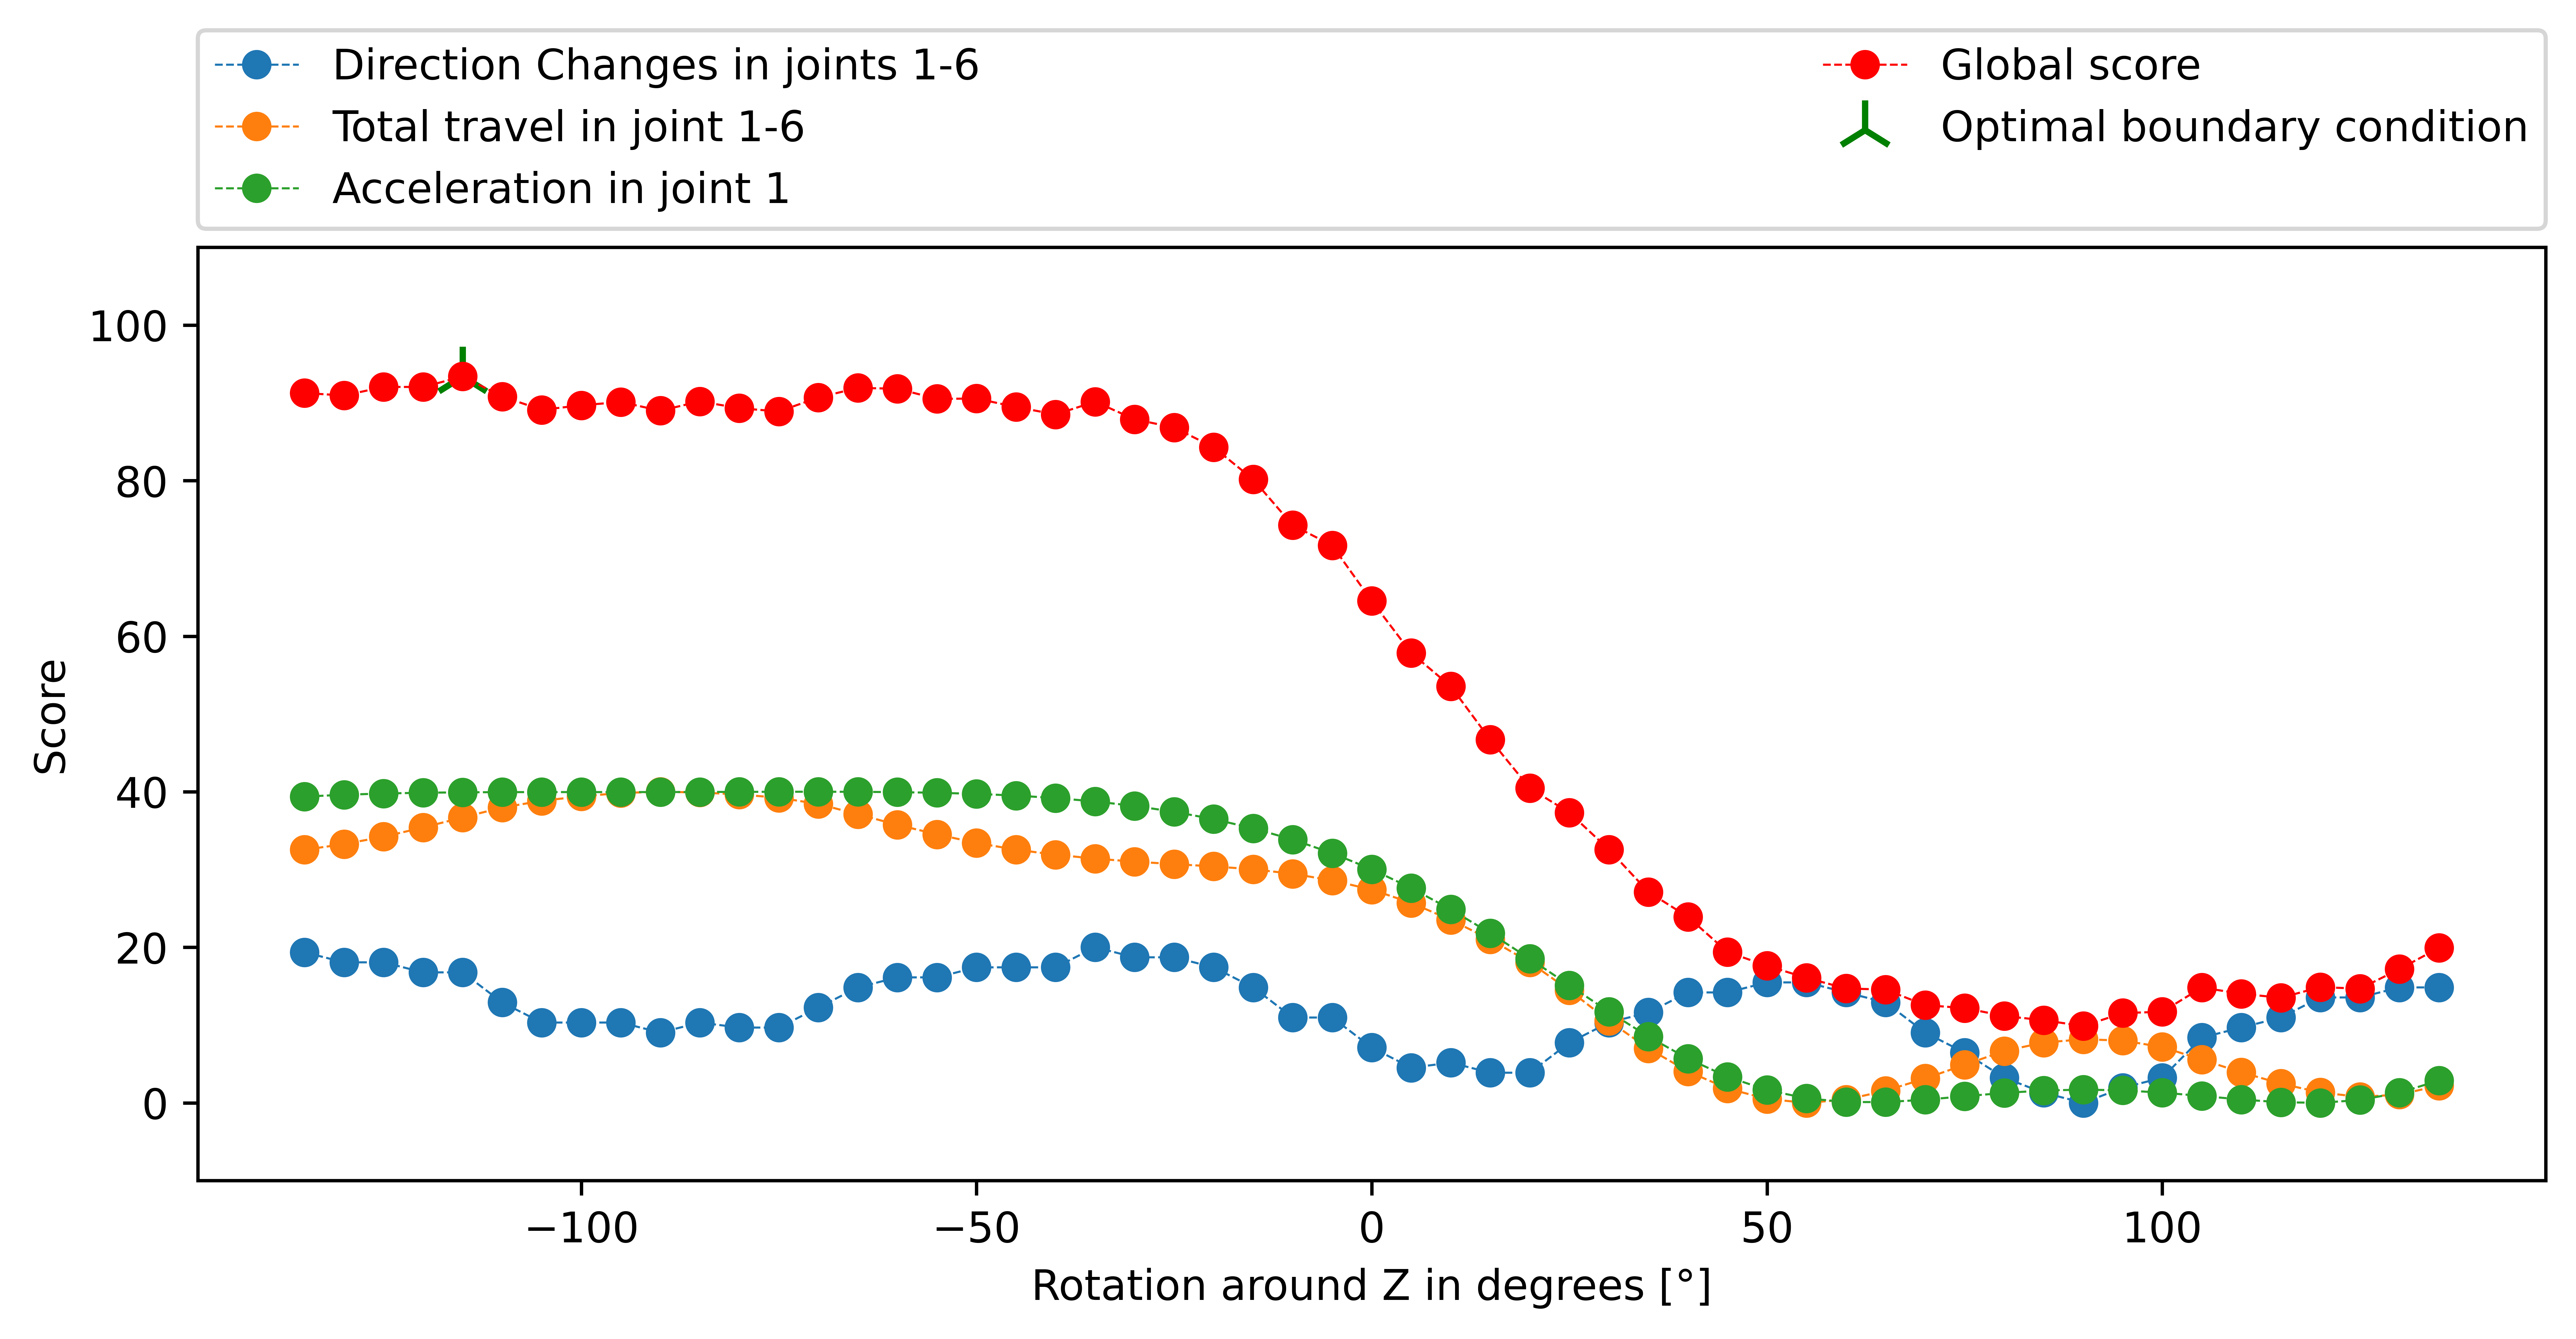
\includegraphics[width=1\textwidth]{figures/best_c_2_combi.png}}
\caption{Global and local scores in toolpath 2 depending on the rotation around Z}
\label{TP2_combi}
\end{figure}
\begin{figure}[H]
\centerline{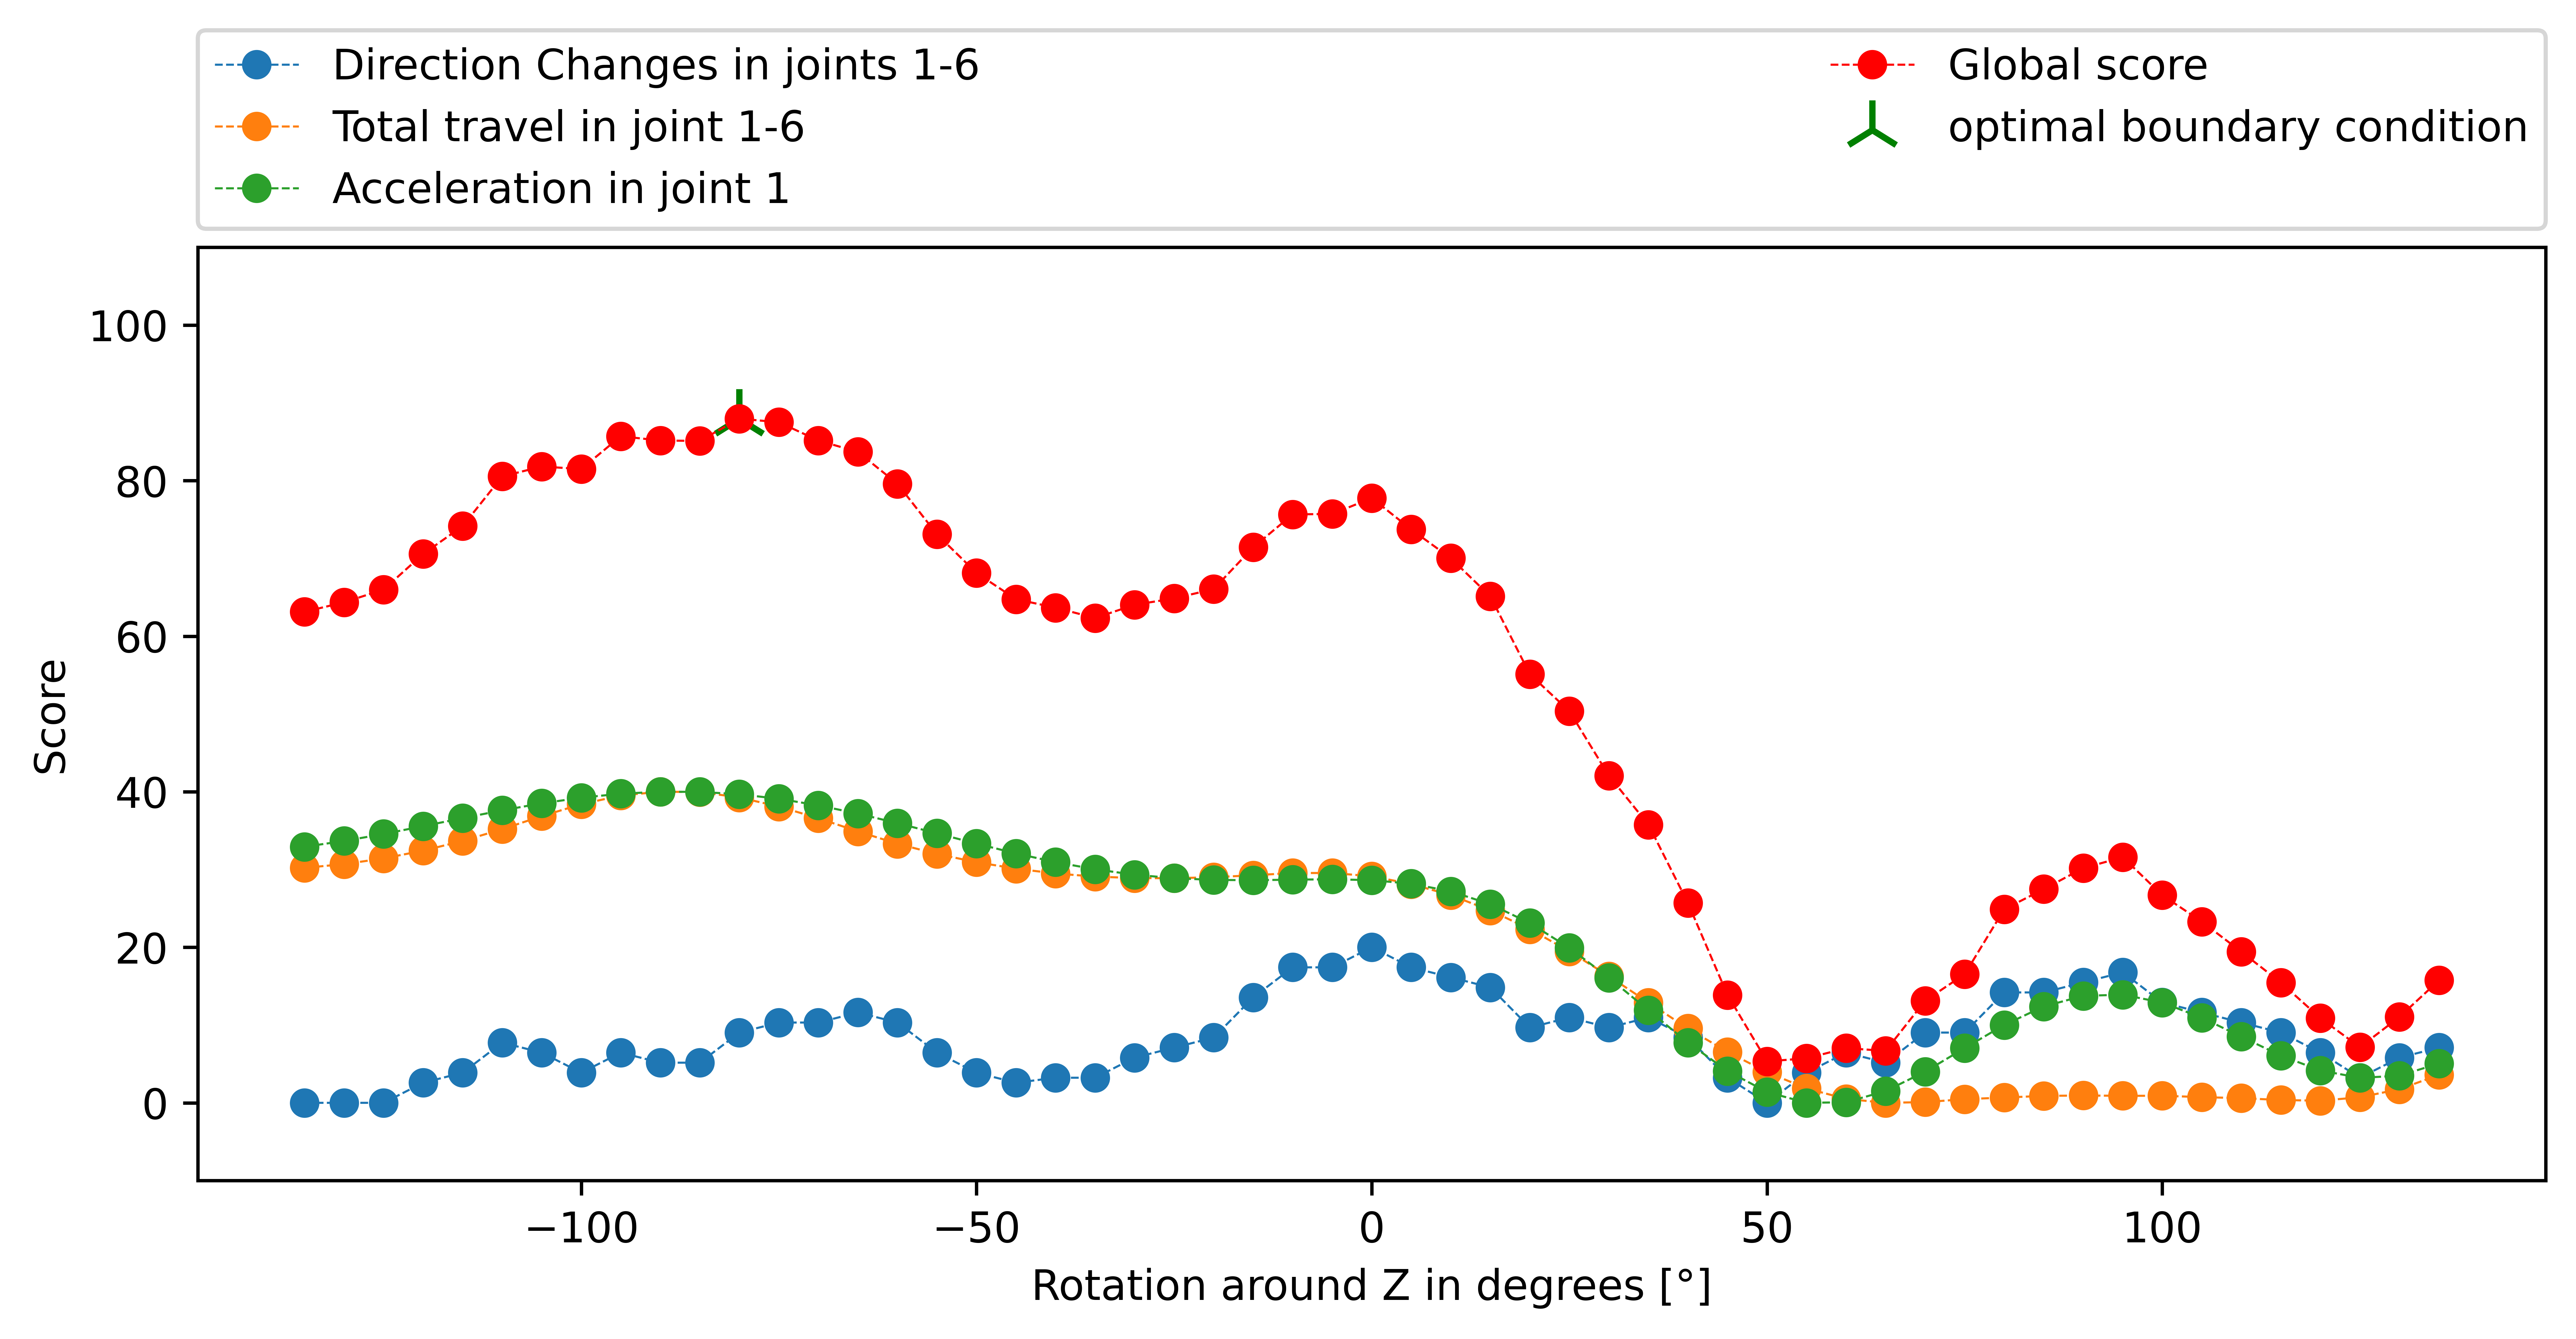
\includegraphics[width=1\textwidth]{figures/best_c_3_combi.png}}
\caption{Global and local scores in toolpath 3 depending on the rotation around Z}
\label{TP3_combi}
\end{figure}

Additionally, it is important to note that when a local score reaches its maximum value, it does not imply that the corresponding process parameter, such as the number of direction changes, becomes zero. Instead, it signifies that the number of direction changes is at its lowest compared to all other analyzed options.

\subsection{Toolpath Evaluation with two Redundant DoF}\label{2RDOF}

To introduce an additional redundant degree of freedom, a rotary-tilt table is simulated. Currently, only the tilting aspect is being analyzed. All coordinates of the toolpath can be rotated by a specified degree around the X-axis. Figure \ref{TP3_0} depicts toolpath 3 with no rotation around the X-axis of its coordinate system. Conversely, Figure \ref{TP3_25} illustrates a rotation of +25 degrees.

\begin{figure}[H]% [H] is so declass\'e!
	\centering
	\begin{minipage}{0.5\textwidth}
		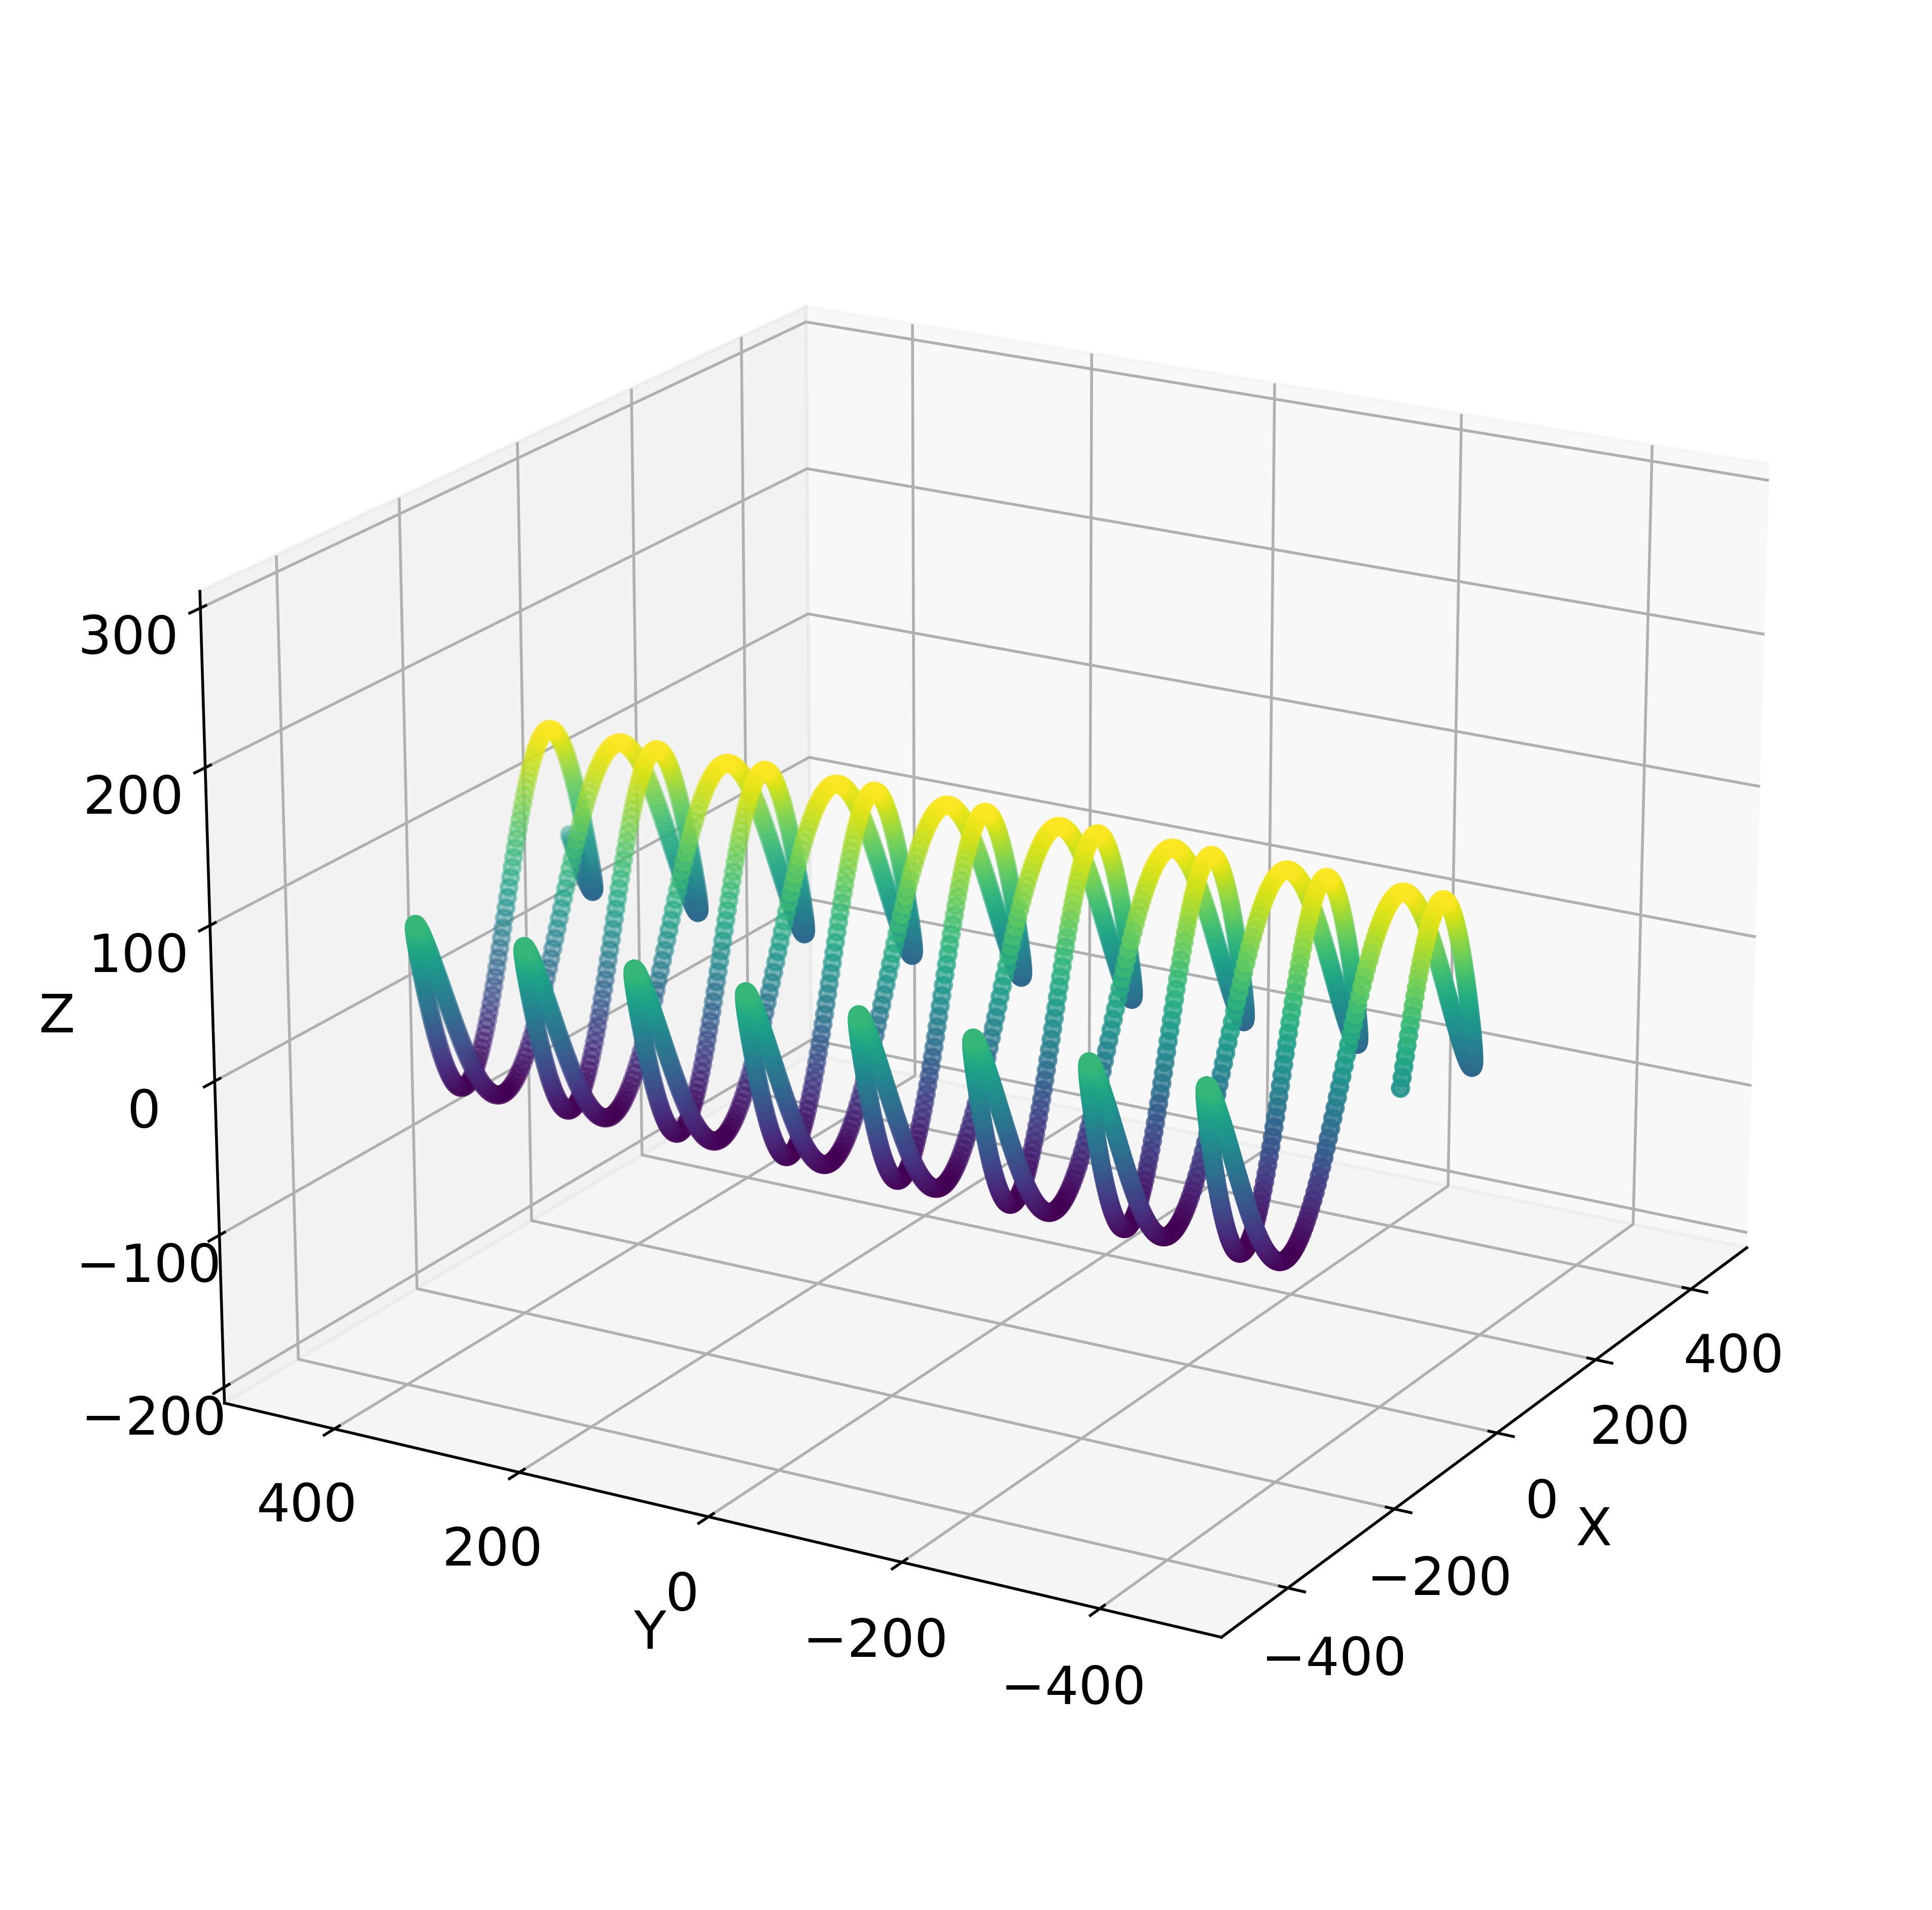
\includegraphics[width=\textwidth]{figures/path3_kipp_0.png}
		\caption{Toolpath 3 with no rotation\newline around the X-axis}
		\label{TP3_0}
	\end{minipage}\hfill
	\begin{minipage}{0.5\textwidth}
		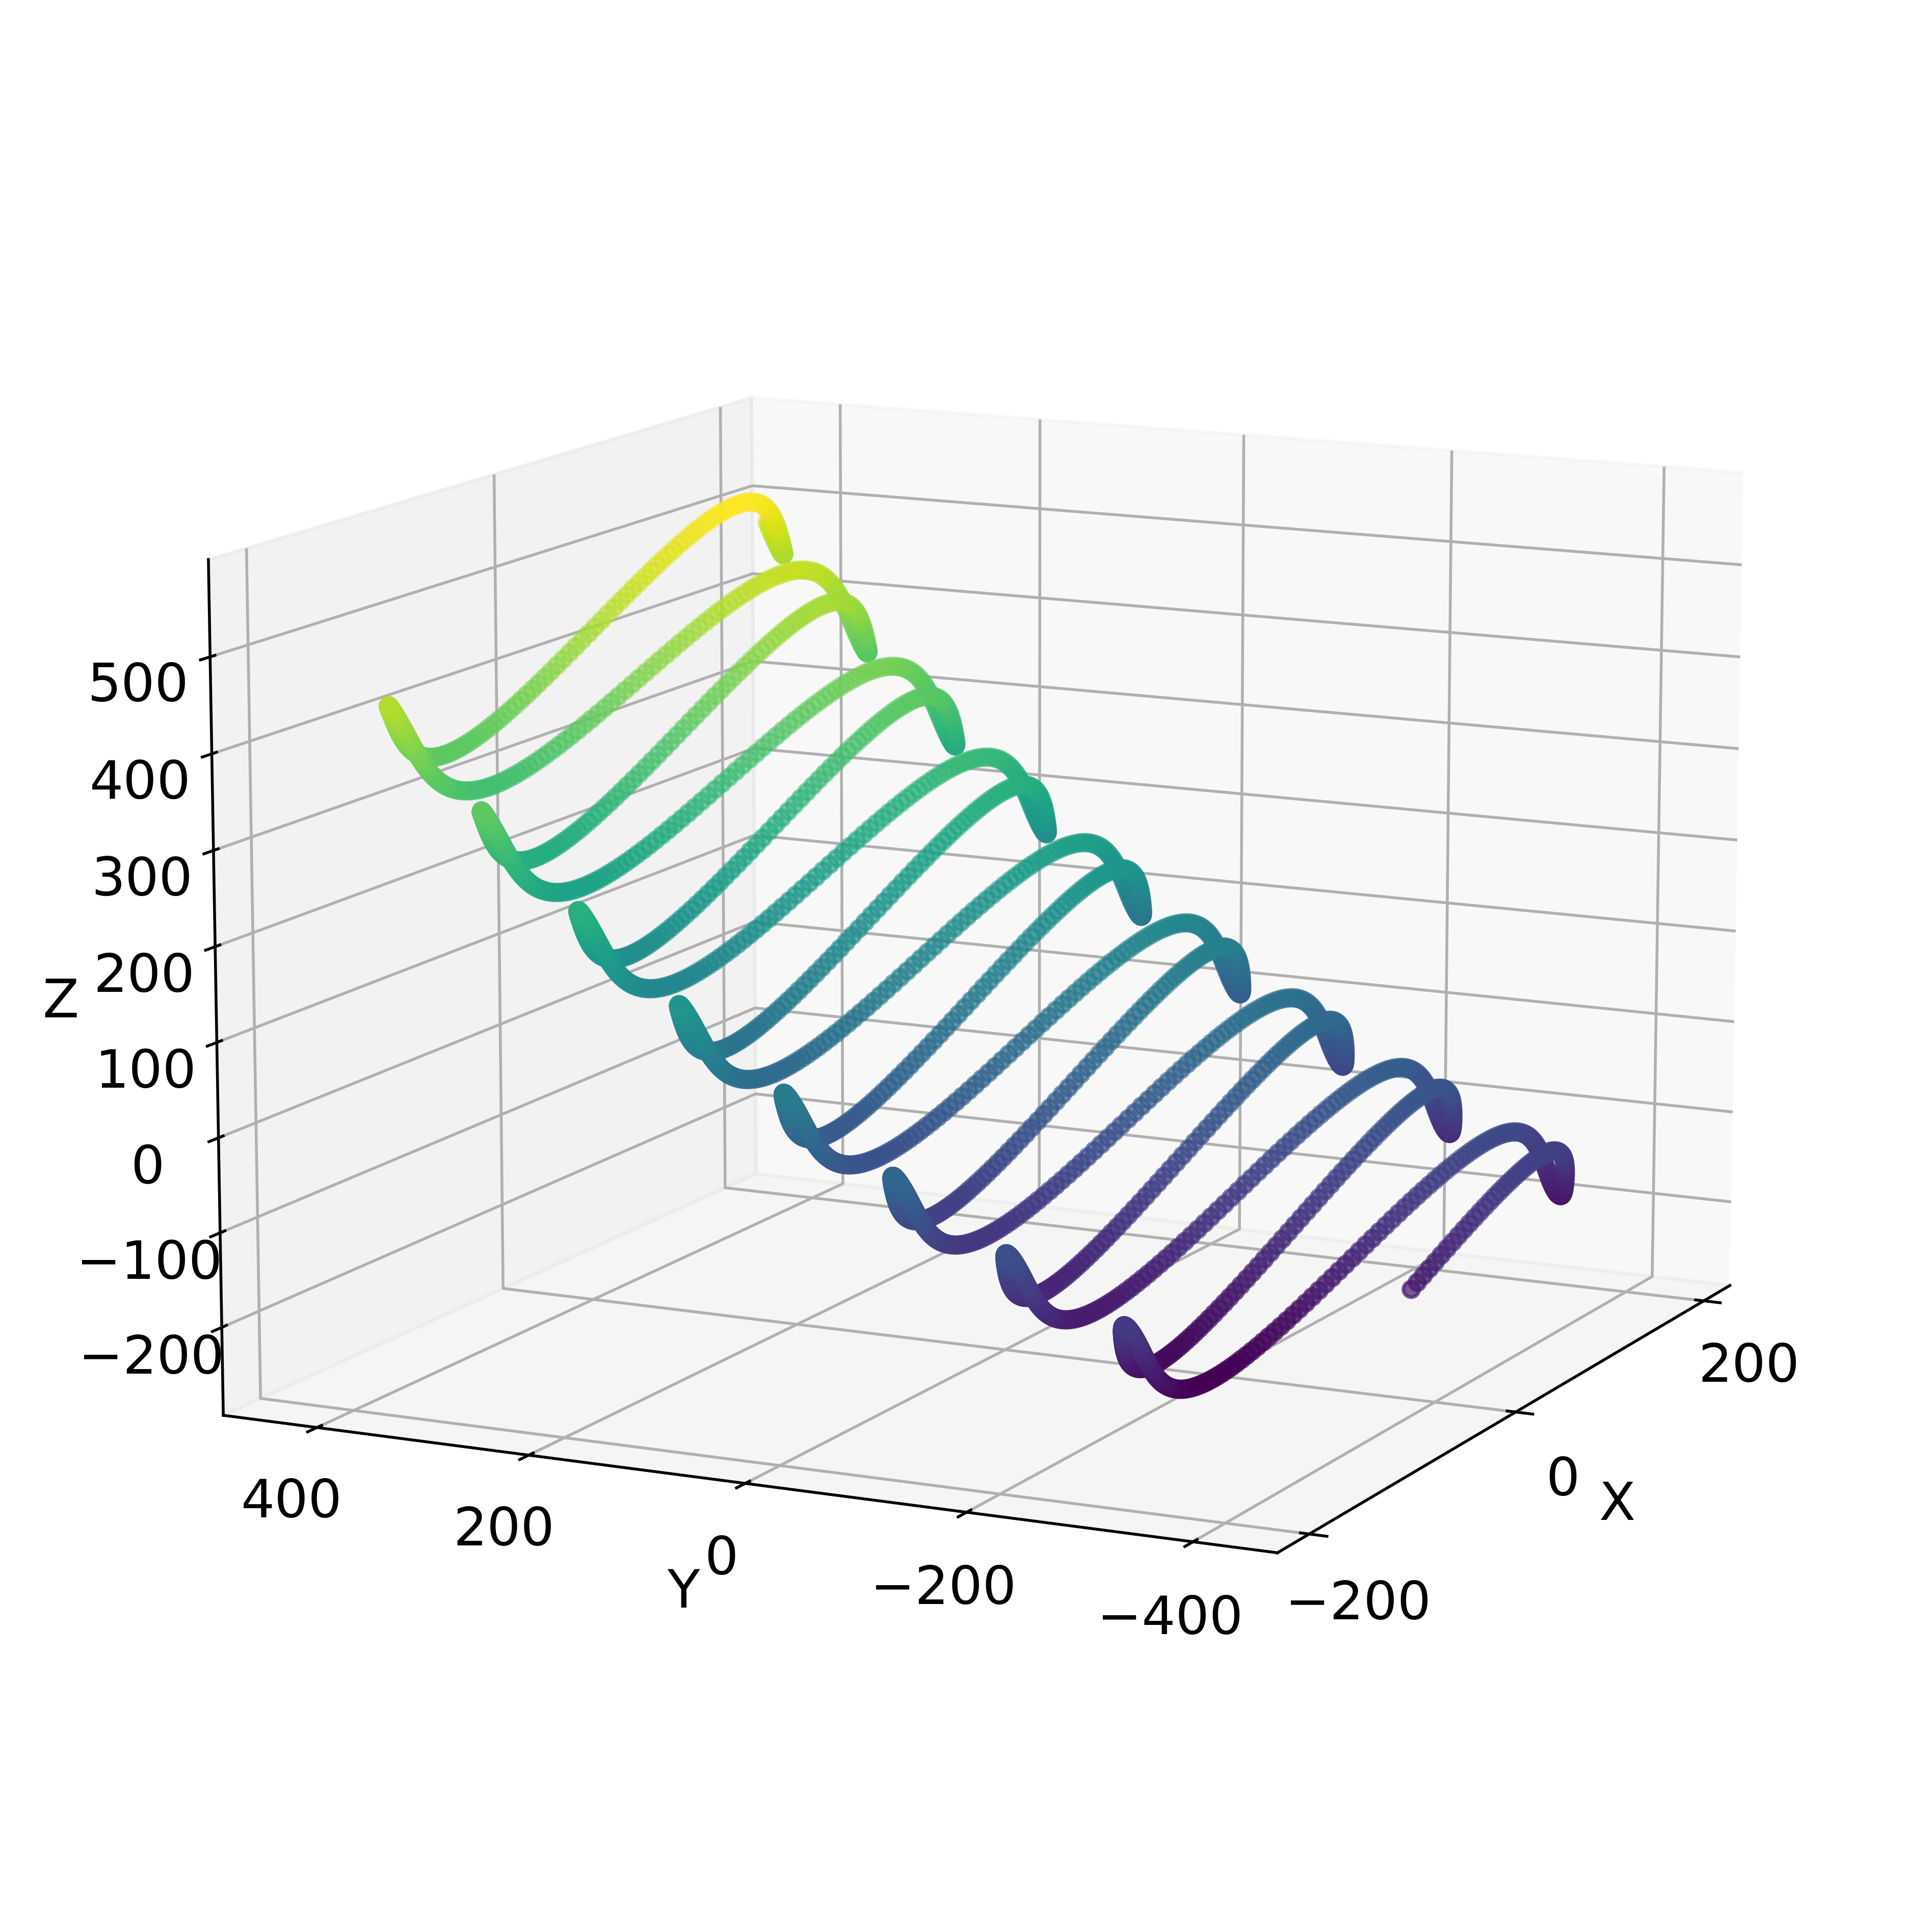
\includegraphics[width=\textwidth]{figures/path3_kipp_25_comparison.png}
		\caption{Toolpath 3 with a rotation\newline of 25 degrees around the X-axis}
		\label{TP3_25}
	\end{minipage}\par
\end{figure}
 

Similar to the previous analysis, the same steps need to be followed. The newly selected process parameters are presented in table \ref{PP_2}. The direction changes of the tilting joints (2+3+5) are combined and treated as one process parameter, weighted with a factor of 0.3. Direction changes in joint 1 and acceleration in joint 4 are considered as individual parameters, both individually weighted with 0.25. The final parameter is the velocity in joint 6, weighted with 0.2.

\begin{table}[H]
	\centering
	\begin{tabular}{||l|l||}
		Process parameters& Importance Factor \\
		\hline
		\hline
		\hline
		Direction changes in joints 2+3+5	&		0.3 \\
		Direction changes in joints 1	&  	0.25 \\
		Acceleration in joint 4	& 		0.25\\
		Velocity in joint 6	& 		0.2\\
		\hline
		\hline
	\end{tabular}
	
	\caption{Selected process parameters and their importance factors for 2 redundant DoF}
	\label{PP_2}
\end{table}


Figure \ref{TP3_25_robot} displays the robot and its orientation while following the tilted toolpath 3. It is crucial to note that since the toolpath is defined in 5 \acrshort{DoF} in its own frame, the frame of the \acrshort{TCP} must also tilt by the same degree as the table. The two redundant \acrshort{DoF} in this case are the rotation around the Z-axis in the frame of the tilted toolpath and the tilting of the toolpath itself. This introduces an additional dimension, as now two parameters can be adapted for the optimization.


\begin{figure}[H]
	\centerline{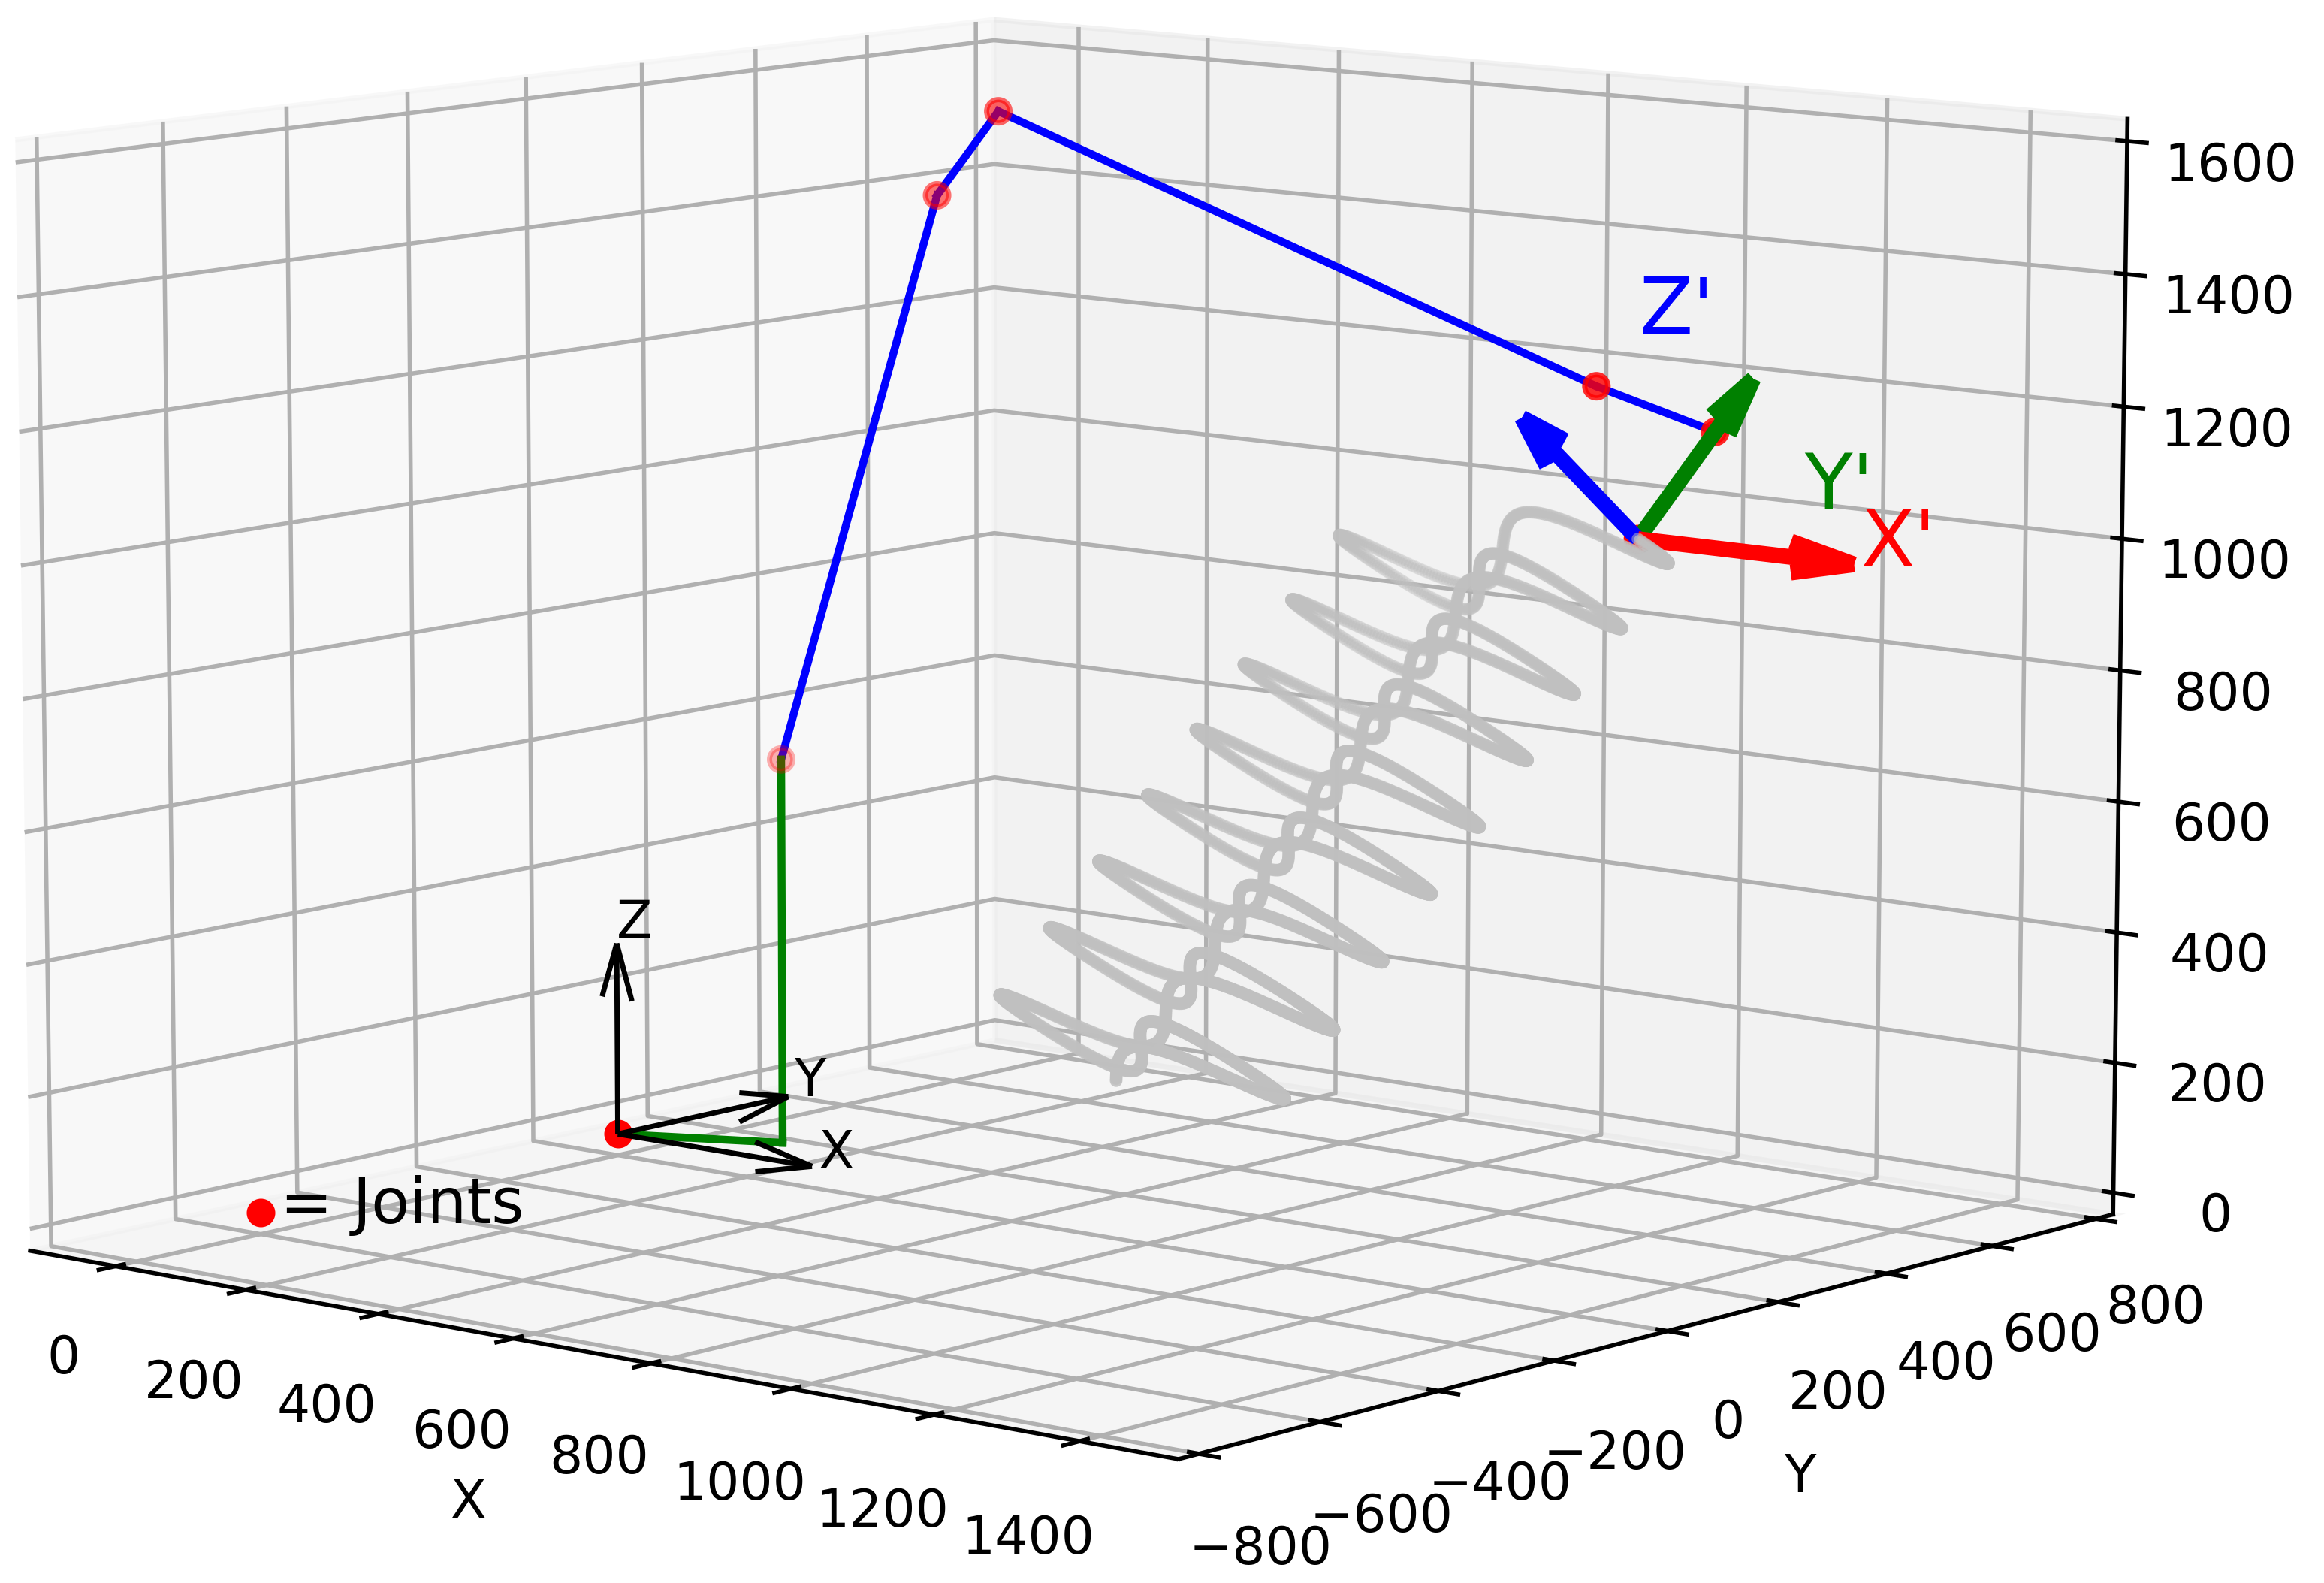
\includegraphics[width=0.9\textwidth]{figures/robotANDpath3_45.png}}
	\caption{Robot following the tilted toolpath 3}
	\label{TP3_25_robot}
\end{figure}

The range of possible tilt positions ranges from -45° to 45° in 2-degree increments. For each tilt position and rotation, the joint angles are generated using inverse kinematics. To speed up the computation, only every third coordinate is utilized in the inverse kinematic algorithm. This reduces the toolpath by 2000 points and speeds up calculation time. On average, it now takes only 10 seconds to calculate the joint positions. A total of 2530 individual combinations are analyzed.

The extracted process parameters are again multiplied by -1, as the objective is to minimize them. Afterward, the Min-Max scaler is applied. The individual values are aggregated and presented in the form of a matrix. The values of this matrix are visualized in figure \ref{best_2D}. The maximum achievable score from all possible combinations is 72.96, visualized by the red cross. This score was attained by setting the table tilt to -3 degrees and the rotation around the Z-axis of the tool to +35 degrees.

The resulting hyperplane exhibits two distinct local maxima. The entire surface displays a smooth curvature, although it appears less smooth in the range from -20 to 45 degrees.


\begin{figure}[H]
	\centerline{\includegraphics[width=1\textwidth]{figures/best_2D_3.png}}
	\caption{Hyperplane representing the global score of toolpath 3}
	\label{best_2D}
\end{figure}


Figure \ref{best_2D_tp2} and Figure \ref{best_2D_tp1} depict the visualization of the global score matrix for toolpath 2 and toolpath 1, respectively.

\begin{figure}[H]
	\centerline{\includegraphics[width=0.7\textwidth]{figures/best_2D_2.png}}
	\caption{Hyperplane representing the global score of toolpath 2}
	\label{best_2D_tp2}
\end{figure}
\begin{figure}[H]
	\centerline{\includegraphics[width=0.7\textwidth]{figures/best_2D_1.png}}
	\caption{Hyperplane representing the global score of toolpath 1}
	\label{best_2D_tp1}
\end{figure}




\newpage
\subsection{Boundary Condition Optimization }
So far, only the analysis of different boundary conditions has been performed by exploring the defined range of the redundant DoF. However, this approach is very time-consuming and scales exponentially with additional redundant degrees of freedom and a finer step size.

To efficiently search this vast space and propose optimal values for the redundant degrees of freedom, a \acrshort{PSO} algorithm is proposed. In this algorithm, individual particles move through the search space by adjusting their positions based on their own best position and the best position found by the swarm. This cooperation allows the particles to explore the search space more effectively and converge towards the best solution.

The first test is conducted using the global score matrix of toolpath 3. Initially, 20 particles are randomly placed on the plane. Their individual scores are determined by the corresponding global score at their respective positions. By increasing the number of particles and iterations, the search space can be analyzed more densely.

Figure \ref{PSO_1} shows the randomly placed particles on the pre-calculates global score matrix.

\begin{figure}[H]
	\centerline{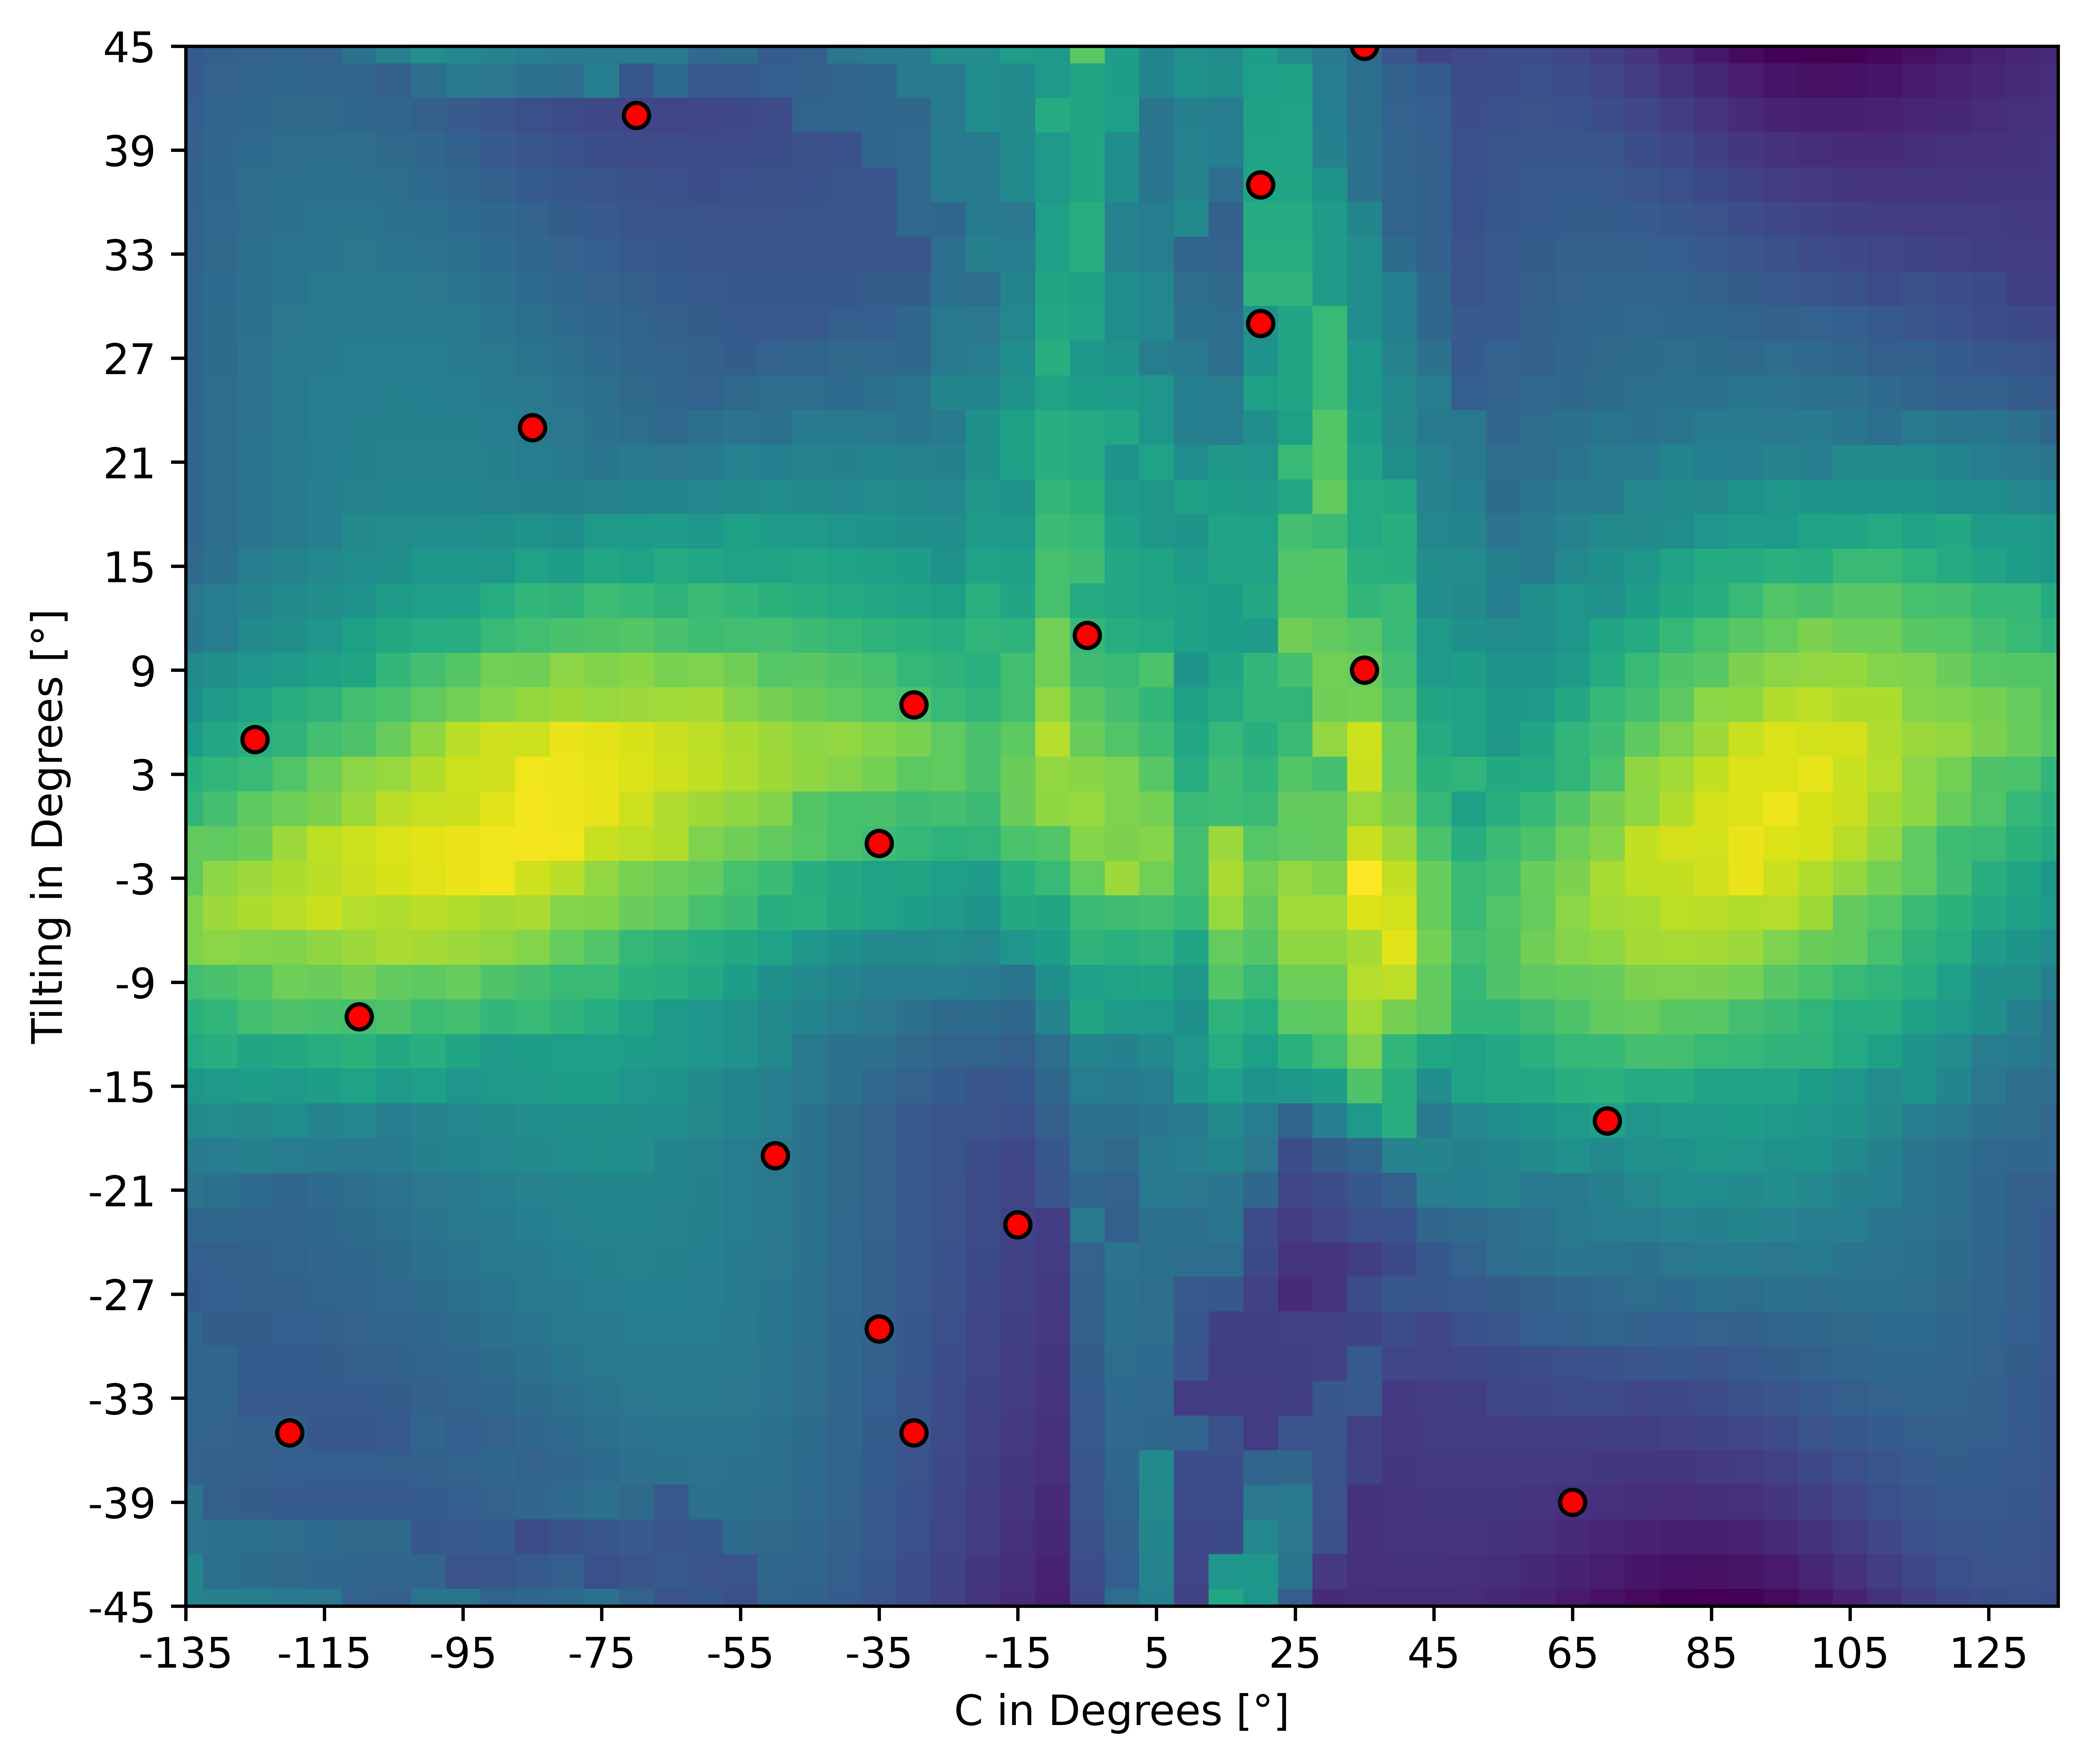
\includegraphics[width=0.8\textwidth]{figures/swarm/3_0.png}}
	\caption{Distributed of particles after the first iteration}
	\label{PSO_1}
\end{figure}


\newpage
Figures \ref{2} to \ref{5} illustrate the convergence of the particles towards the identified maximum. This convergence is achieved within 5 iterations. It is noteworthy that the best position of all 5 particles matches the global maximum, as mentioned in Chapter \ref{2RDOF}. This example demonstrates that it is possible to explore a high-dimensional space without the need to compute all possible combinations.


\begin{figure}[H]
	\centering
	\begin{minipage}{0.5\textwidth}
		\includegraphics[width=\textwidth]{figures/swarm/3_2.png}
		\caption{PSO Iteration 2 on toolpath 3}
		\label{2}
	\end{minipage}\hfill
	\begin{minipage}{0.5\textwidth}
		\includegraphics[width=\textwidth]{figures/swarm/3_3.png}
		\caption{PSO Iteration 3 on toolpath 3}
		\label{3}
	\end{minipage}\par
\end{figure}	


\begin{figure}[H]	
		\centering
	\begin{minipage}{0.5\textwidth}
		\includegraphics[width=\textwidth]{figures/swarm/3_4.png}
		\caption{PSO Iteration 4 on toolpath 3}
		\label{4}
	\end{minipage}\hfill
	\begin{minipage}{0.5\textwidth}
		\includegraphics[width=\textwidth]{figures/swarm/3_5.png}
		\caption{PSO Iteration 5 on toolpath 3}
		\label{5}
	\end{minipage}\par
\end{figure}

One crucial factor in this test is that the scores have already been calculated. The global score matrix is determined based on all possible combinations of different boundary conditions. However, in the intended scenario where this method is used to find the optimal boundary condition, such a matrix does not exist.
\newpage

Therefore, the scores of individual positions need to be compared relative to each other at each iteration, taking into account the previous iterations. This method is depicted in Figure \ref{swarmloop}. Initially, a predetermined number of particles is randomly placed on the plane, with the X and Y values representing the selected boundary conditions. For each selected boundary condition, the joint angles are calculated using the inverse kinematic approach. Subsequently, the analyzed process parameters are extracted and the joint angles are stored. The score for each current position is calculated relative to all stored toolpaths.

It is possible that a particle had a position with a significantly higher score compared to the other available toolpaths in an early iteration. Therefore, after each iteration, it is necessary to update the score of the particle's most optimal position, as more boundary conditions are analyzed. This is done to ensure that an initially relative score, which may have been mistakenly chosen as the best, does not influence the subsequent search directions.

\begin{figure}[H]
	\centerline{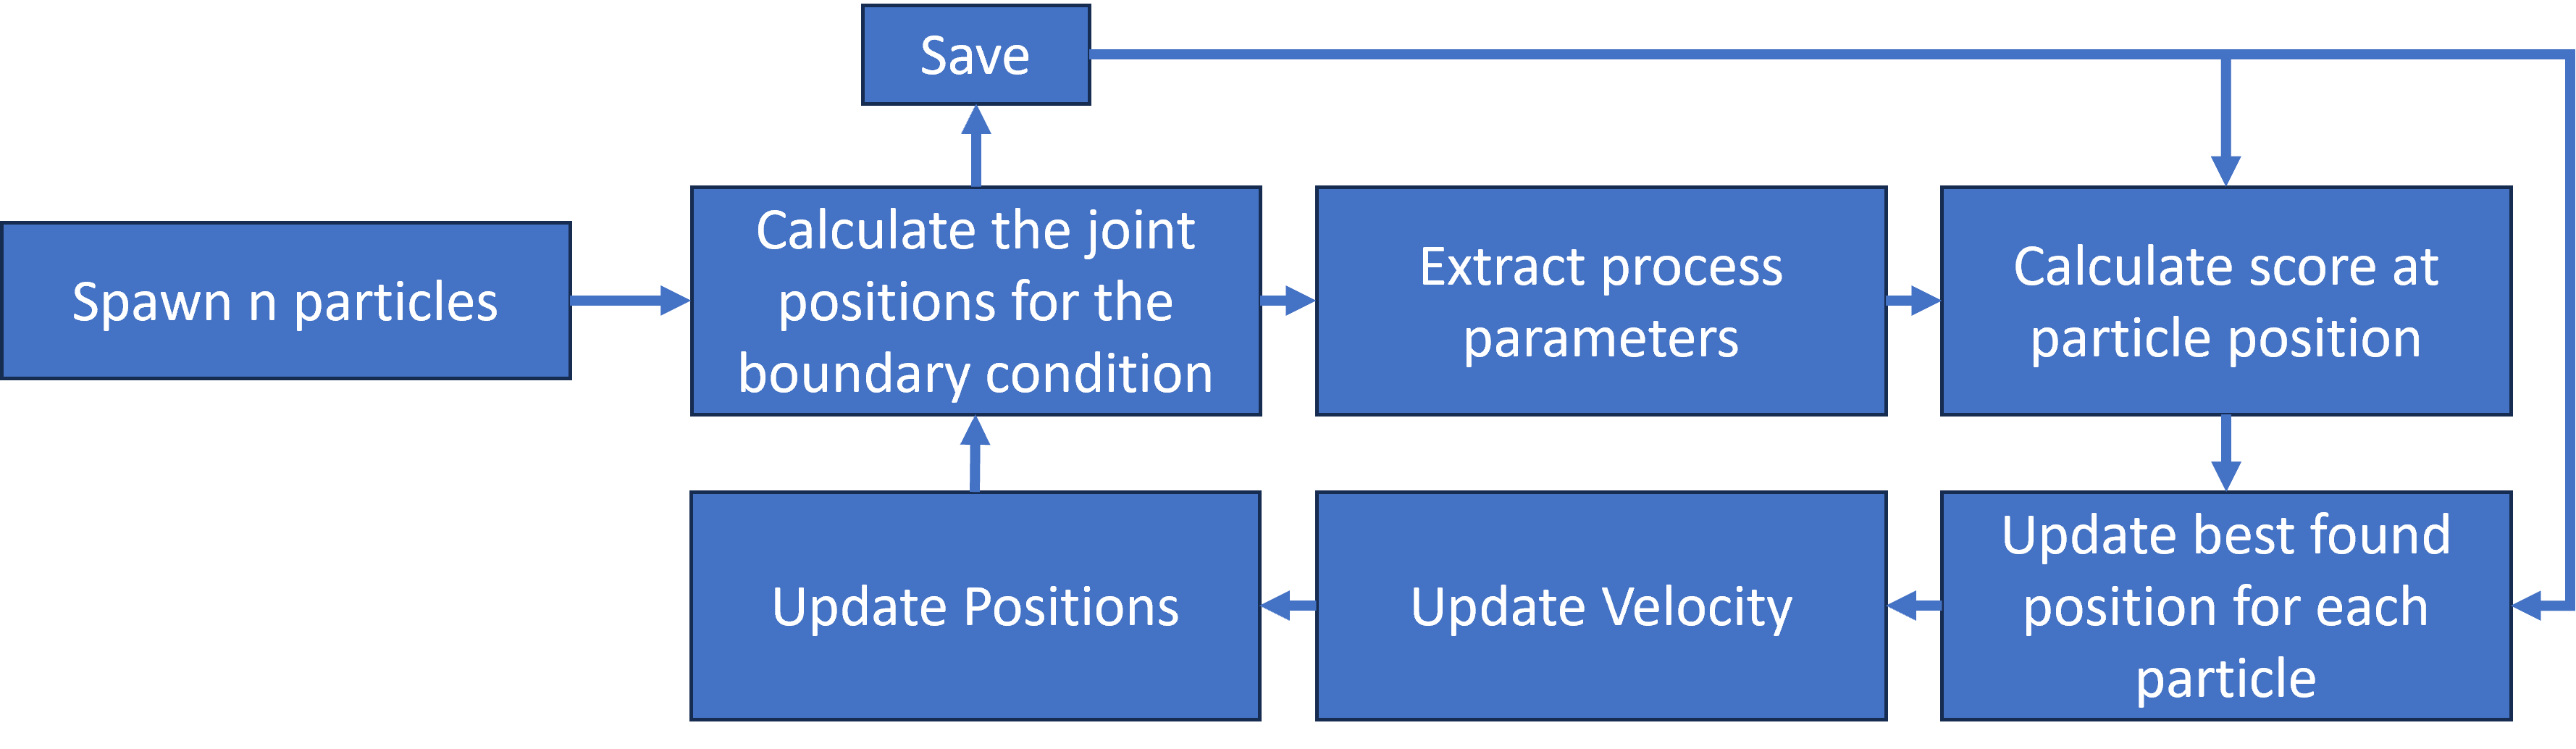
\includegraphics[width=1\textwidth]{figures/swarmloop.png}}
	\caption{PSO-Loop}
	\label{swarmloop}
\end{figure}

Utilizing this approach, the following results have been obtained. It is crucial to note that the colors from the global score matrix are not accessible to the \acrshort{PSO} algorithm. They are solely used for evaluating the behavior of the particles and aiding in visualization.

Figures \ref{1_true} to \ref{4_true} demonstrate the progression of the individual particles. The green circle represents the overall best position discovered by the particles thus far.

\begin{figure}[H]
	\centering
	\begin{minipage}{0.5\textwidth}
		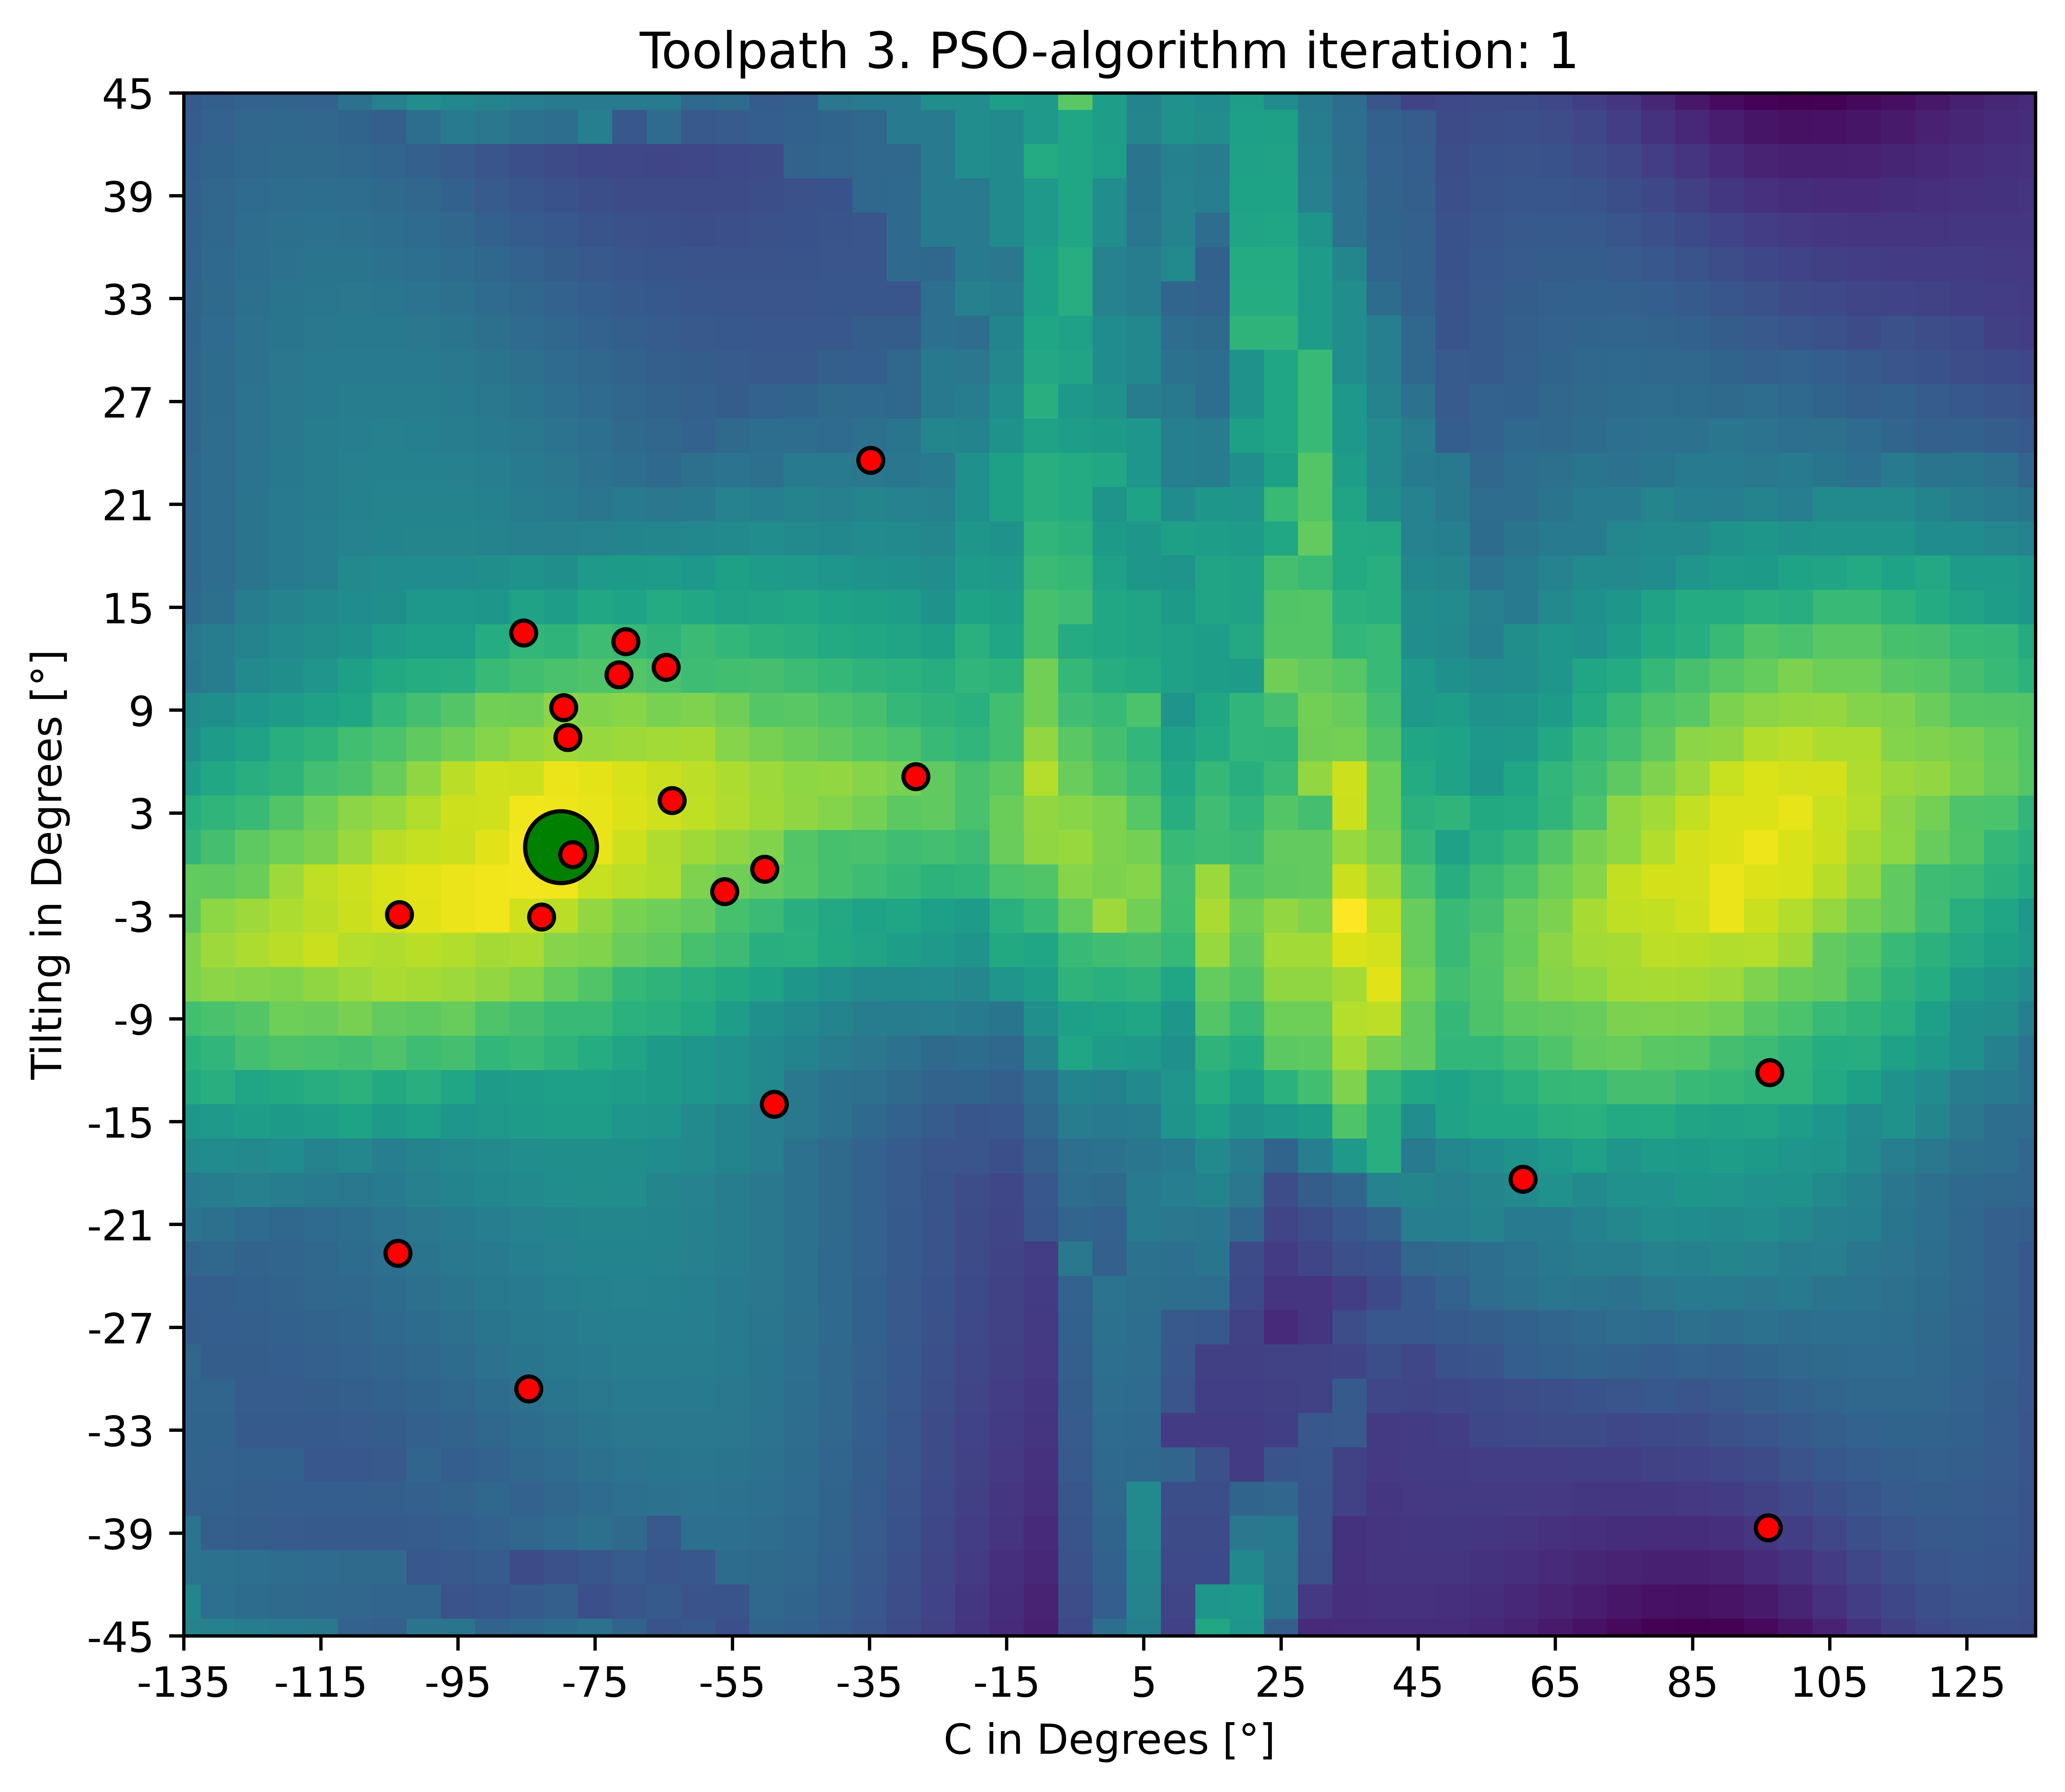
\includegraphics[width=\textwidth]{figures/swarm_true/3_1.png}
		\caption{PSO Iteration 1 on toolpath 3}
		\label{1_true}
	\end{minipage}\hfill
	\begin{minipage}{0.5\textwidth}
		\includegraphics[width=\textwidth]{figures/swarm_true/3_2.png}
		\caption{PSO Iteration 2 on toolpath 3}
		\label{2_true}
	\end{minipage}\par
\end{figure}	

\begin{figure}[H]	
	\centering
	\begin{minipage}{0.5\textwidth}
		\includegraphics[width=\textwidth]{figures/swarm_true/3_3.png}
		\caption{PSO Iteration 3 on toolpath 3}
		\label{3_true}
	\end{minipage}\hfill
	\begin{minipage}{0.5\textwidth}
		\includegraphics[width=\textwidth]{figures/swarm_true/3_4.png}
		\caption{PSO Iteration 4 on toolpath 3}
		\label{4_true}
	\end{minipage}\par
\end{figure}

Figure \ref{5_true} illustrates the positions of the particles after the fifth and final iteration.

\begin{figure}[H]
	\centerline{\includegraphics[width=0.9\textwidth]{figures/swarm_true/3_5.png}}
	\caption{PSO iteration 5 on toolpath 3}
	\label{5_true}
\end{figure}

\newpage
Figures \ref{tp1_0} through \ref{tp1_5} and Figures \ref{tp2_0} and \ref{tp2_5} showcase the initial and final positions of the particles when analyzing the first and second toolpath, respectively. In both cases, the PSO algorithm successfully converged towards the optimal boundary condition.

\begin{figure}[H]	
	\centering
	\begin{minipage}{0.5\textwidth}
		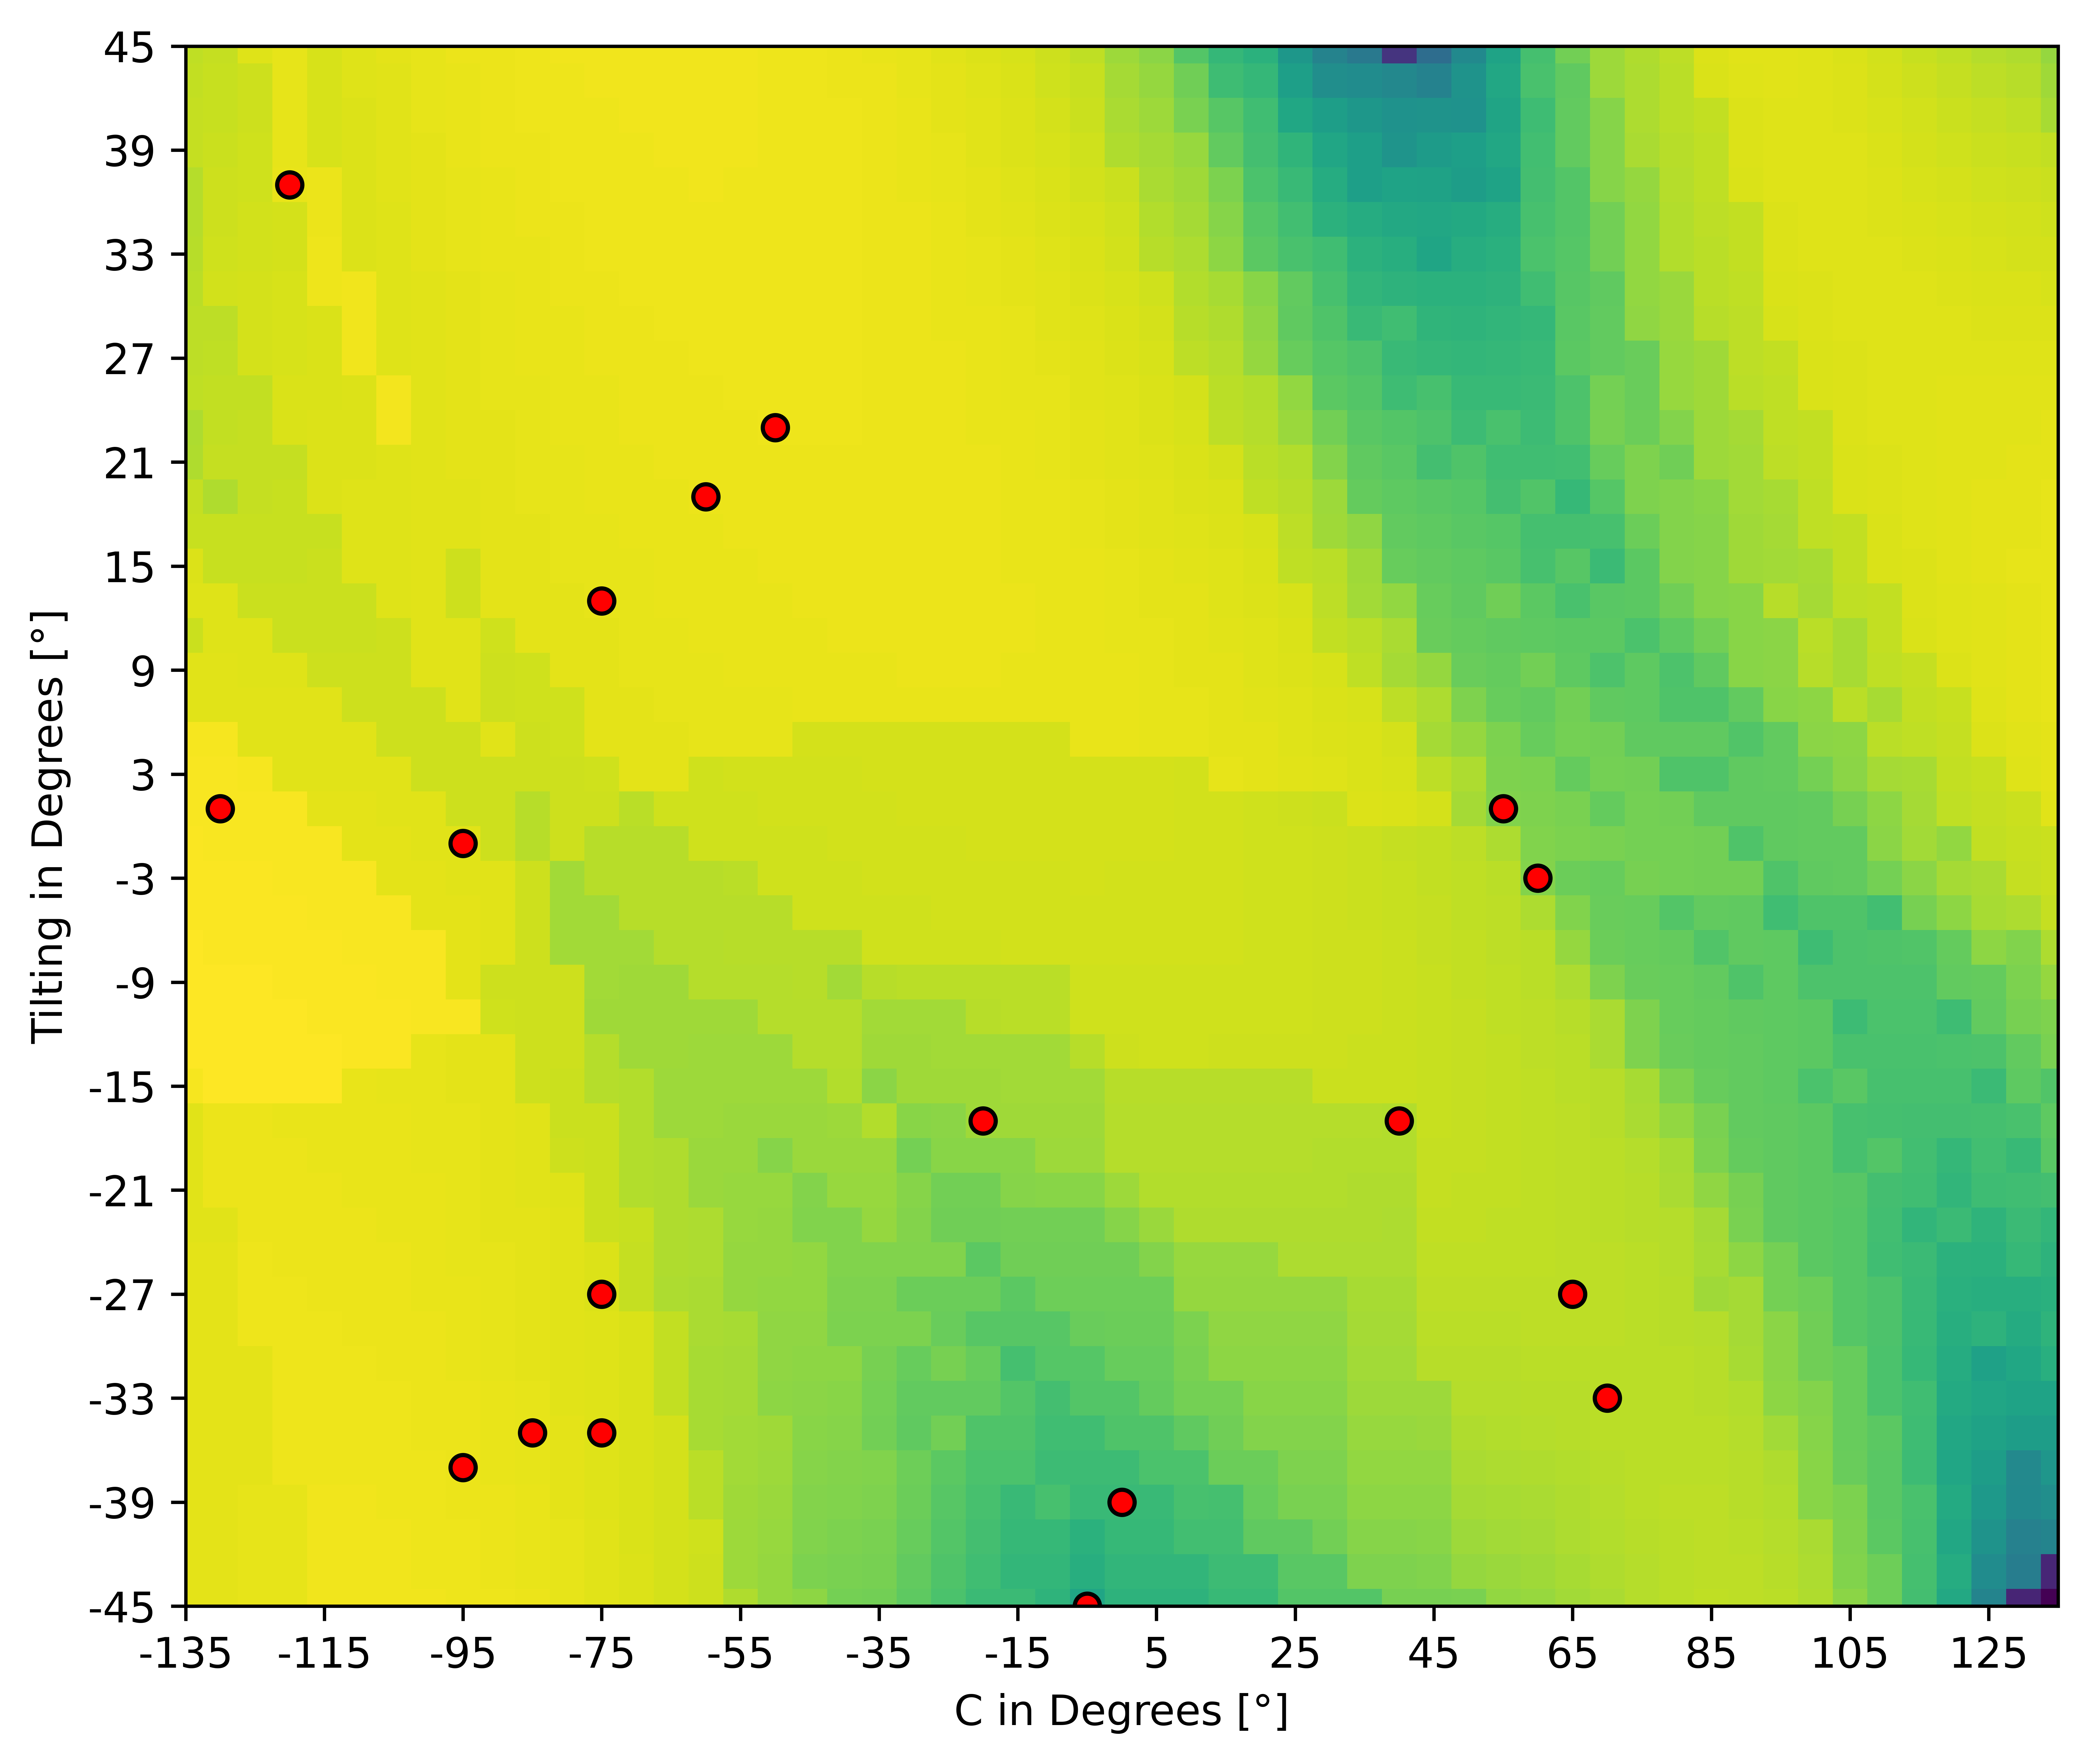
\includegraphics[width=\textwidth]{figures/swarm_true/1_0.png}
		\caption{PSO Initial position toolpath 1}
		\label{tp1_0}
	\end{minipage}\hfill
	\begin{minipage}{0.5\textwidth}
		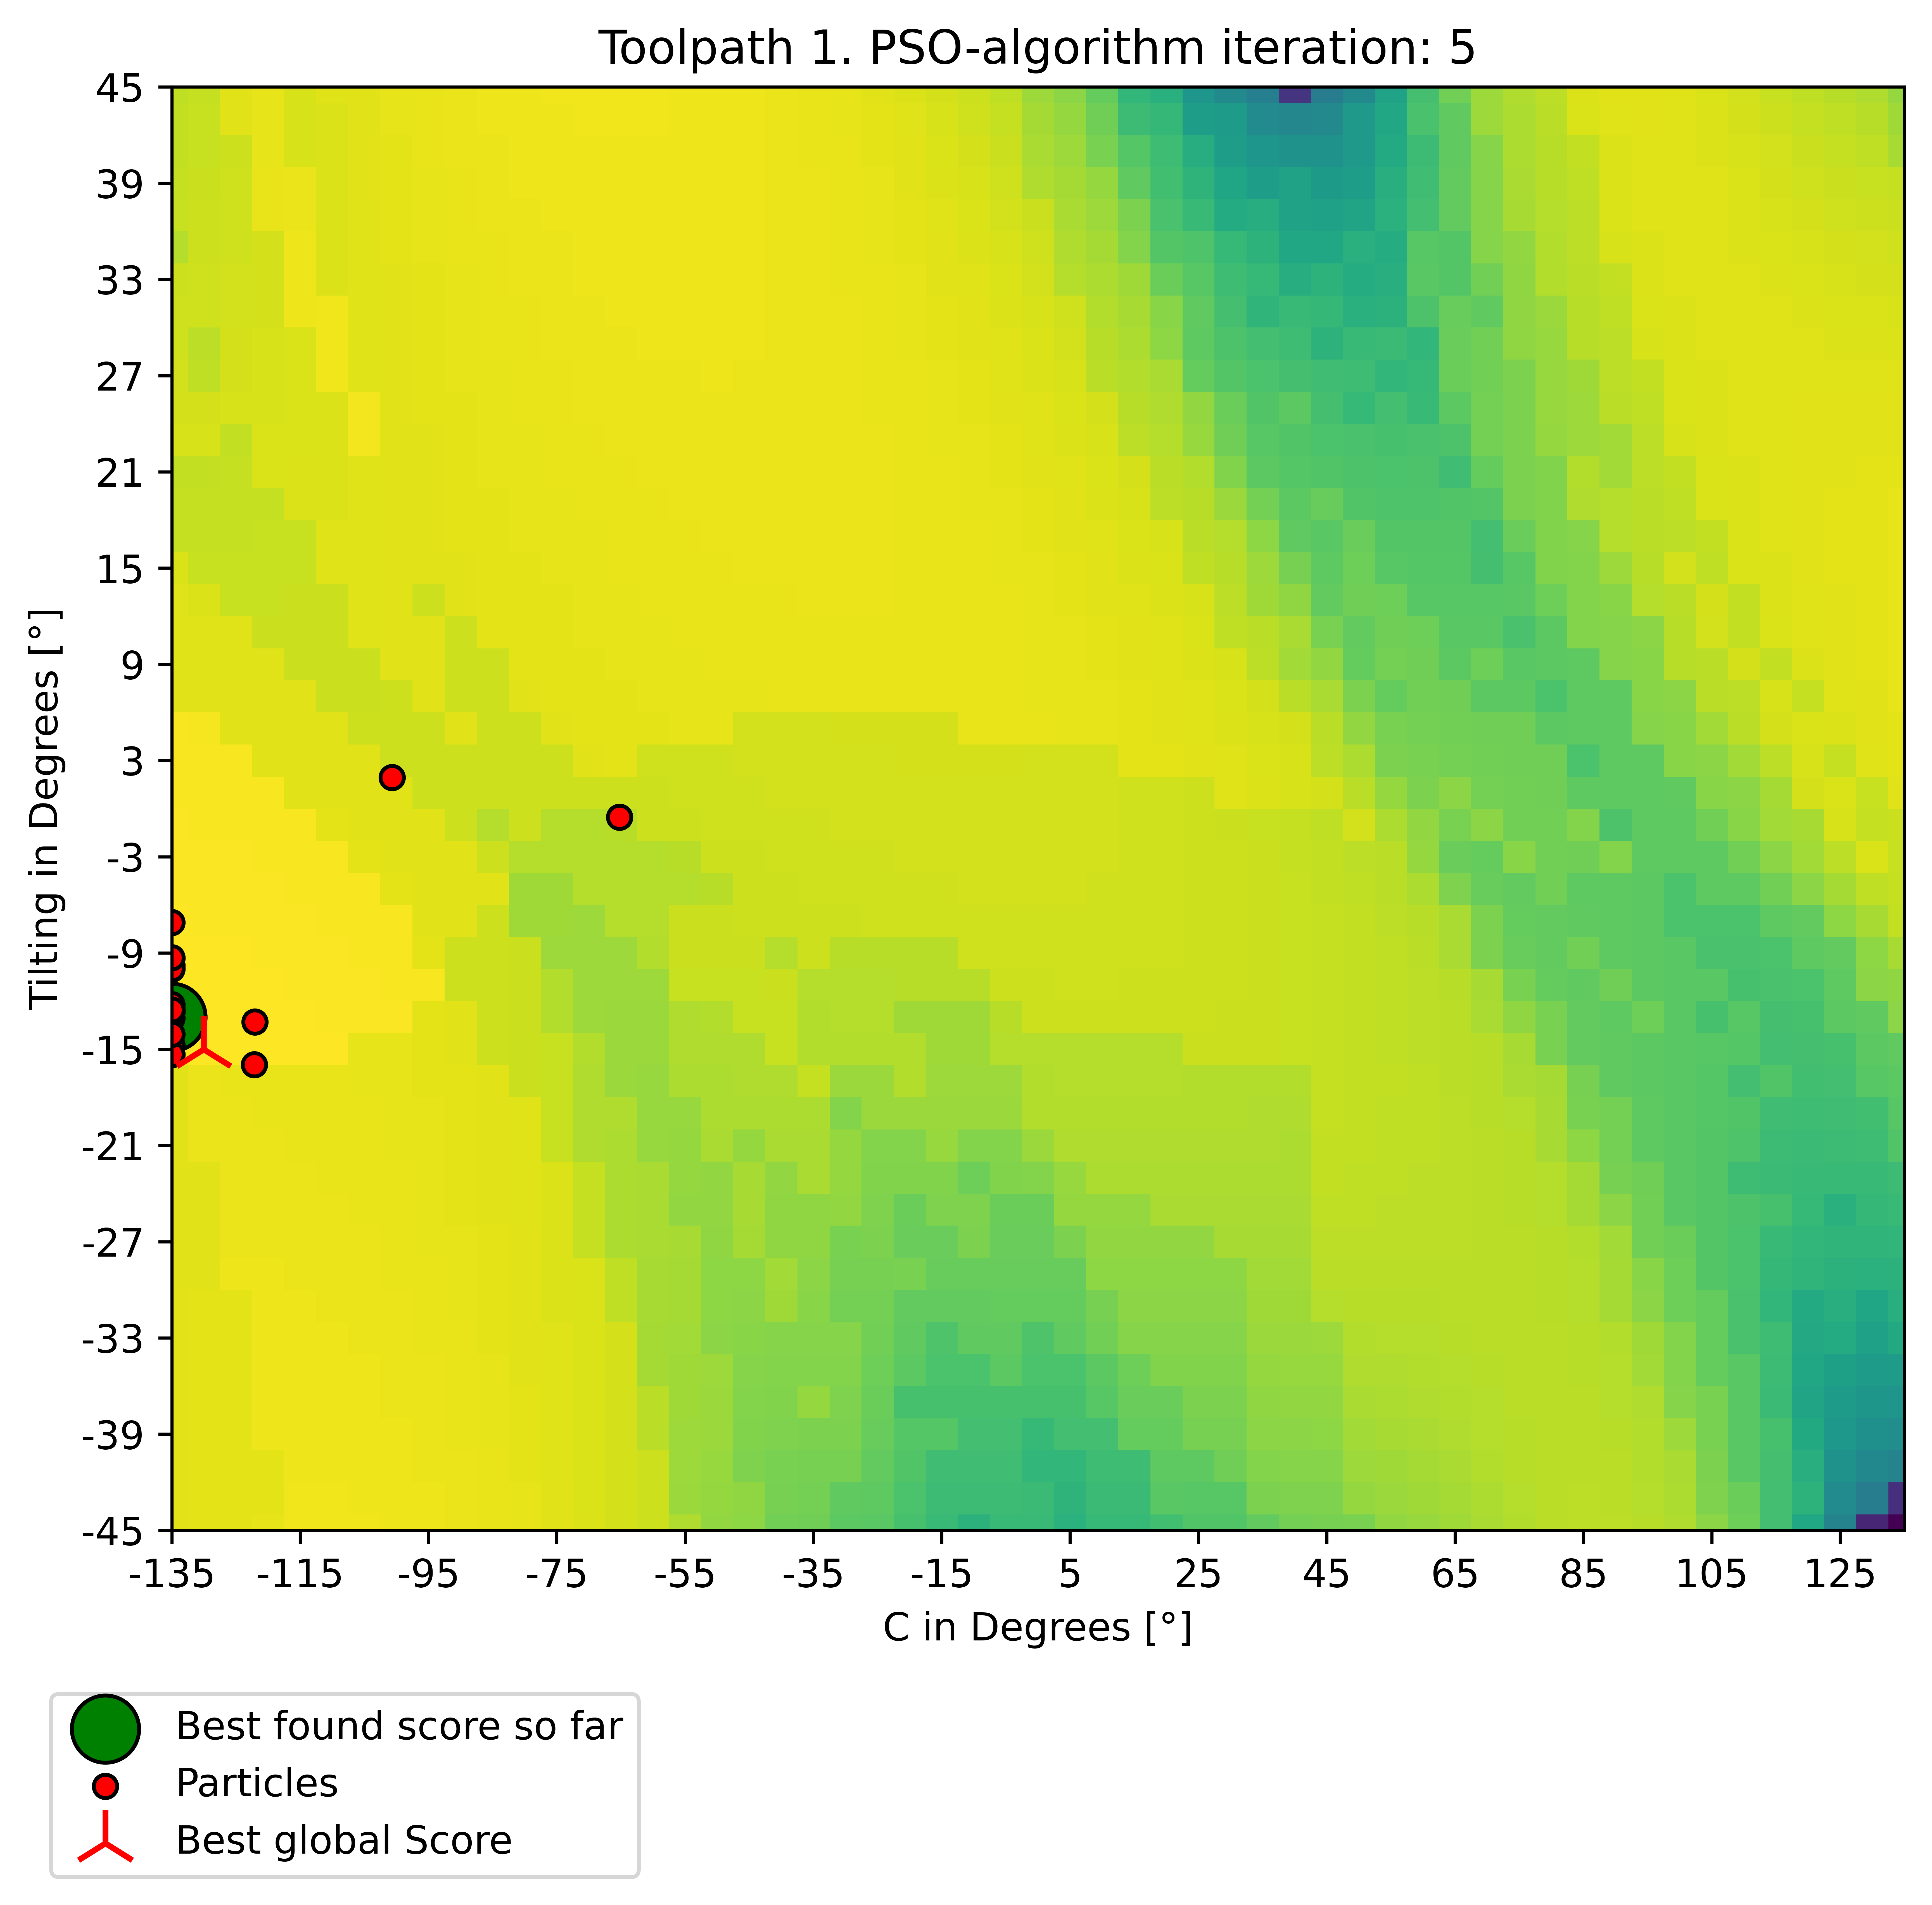
\includegraphics[width=\textwidth]{figures/swarm_true/1_5.png}
		\caption{PSO Iteration 5 on toolpath 1}
		\label{tp1_5}
	\end{minipage}\par
\end{figure}


\begin{figure}[H]	
	\centering
	\begin{minipage}{0.5\textwidth}
		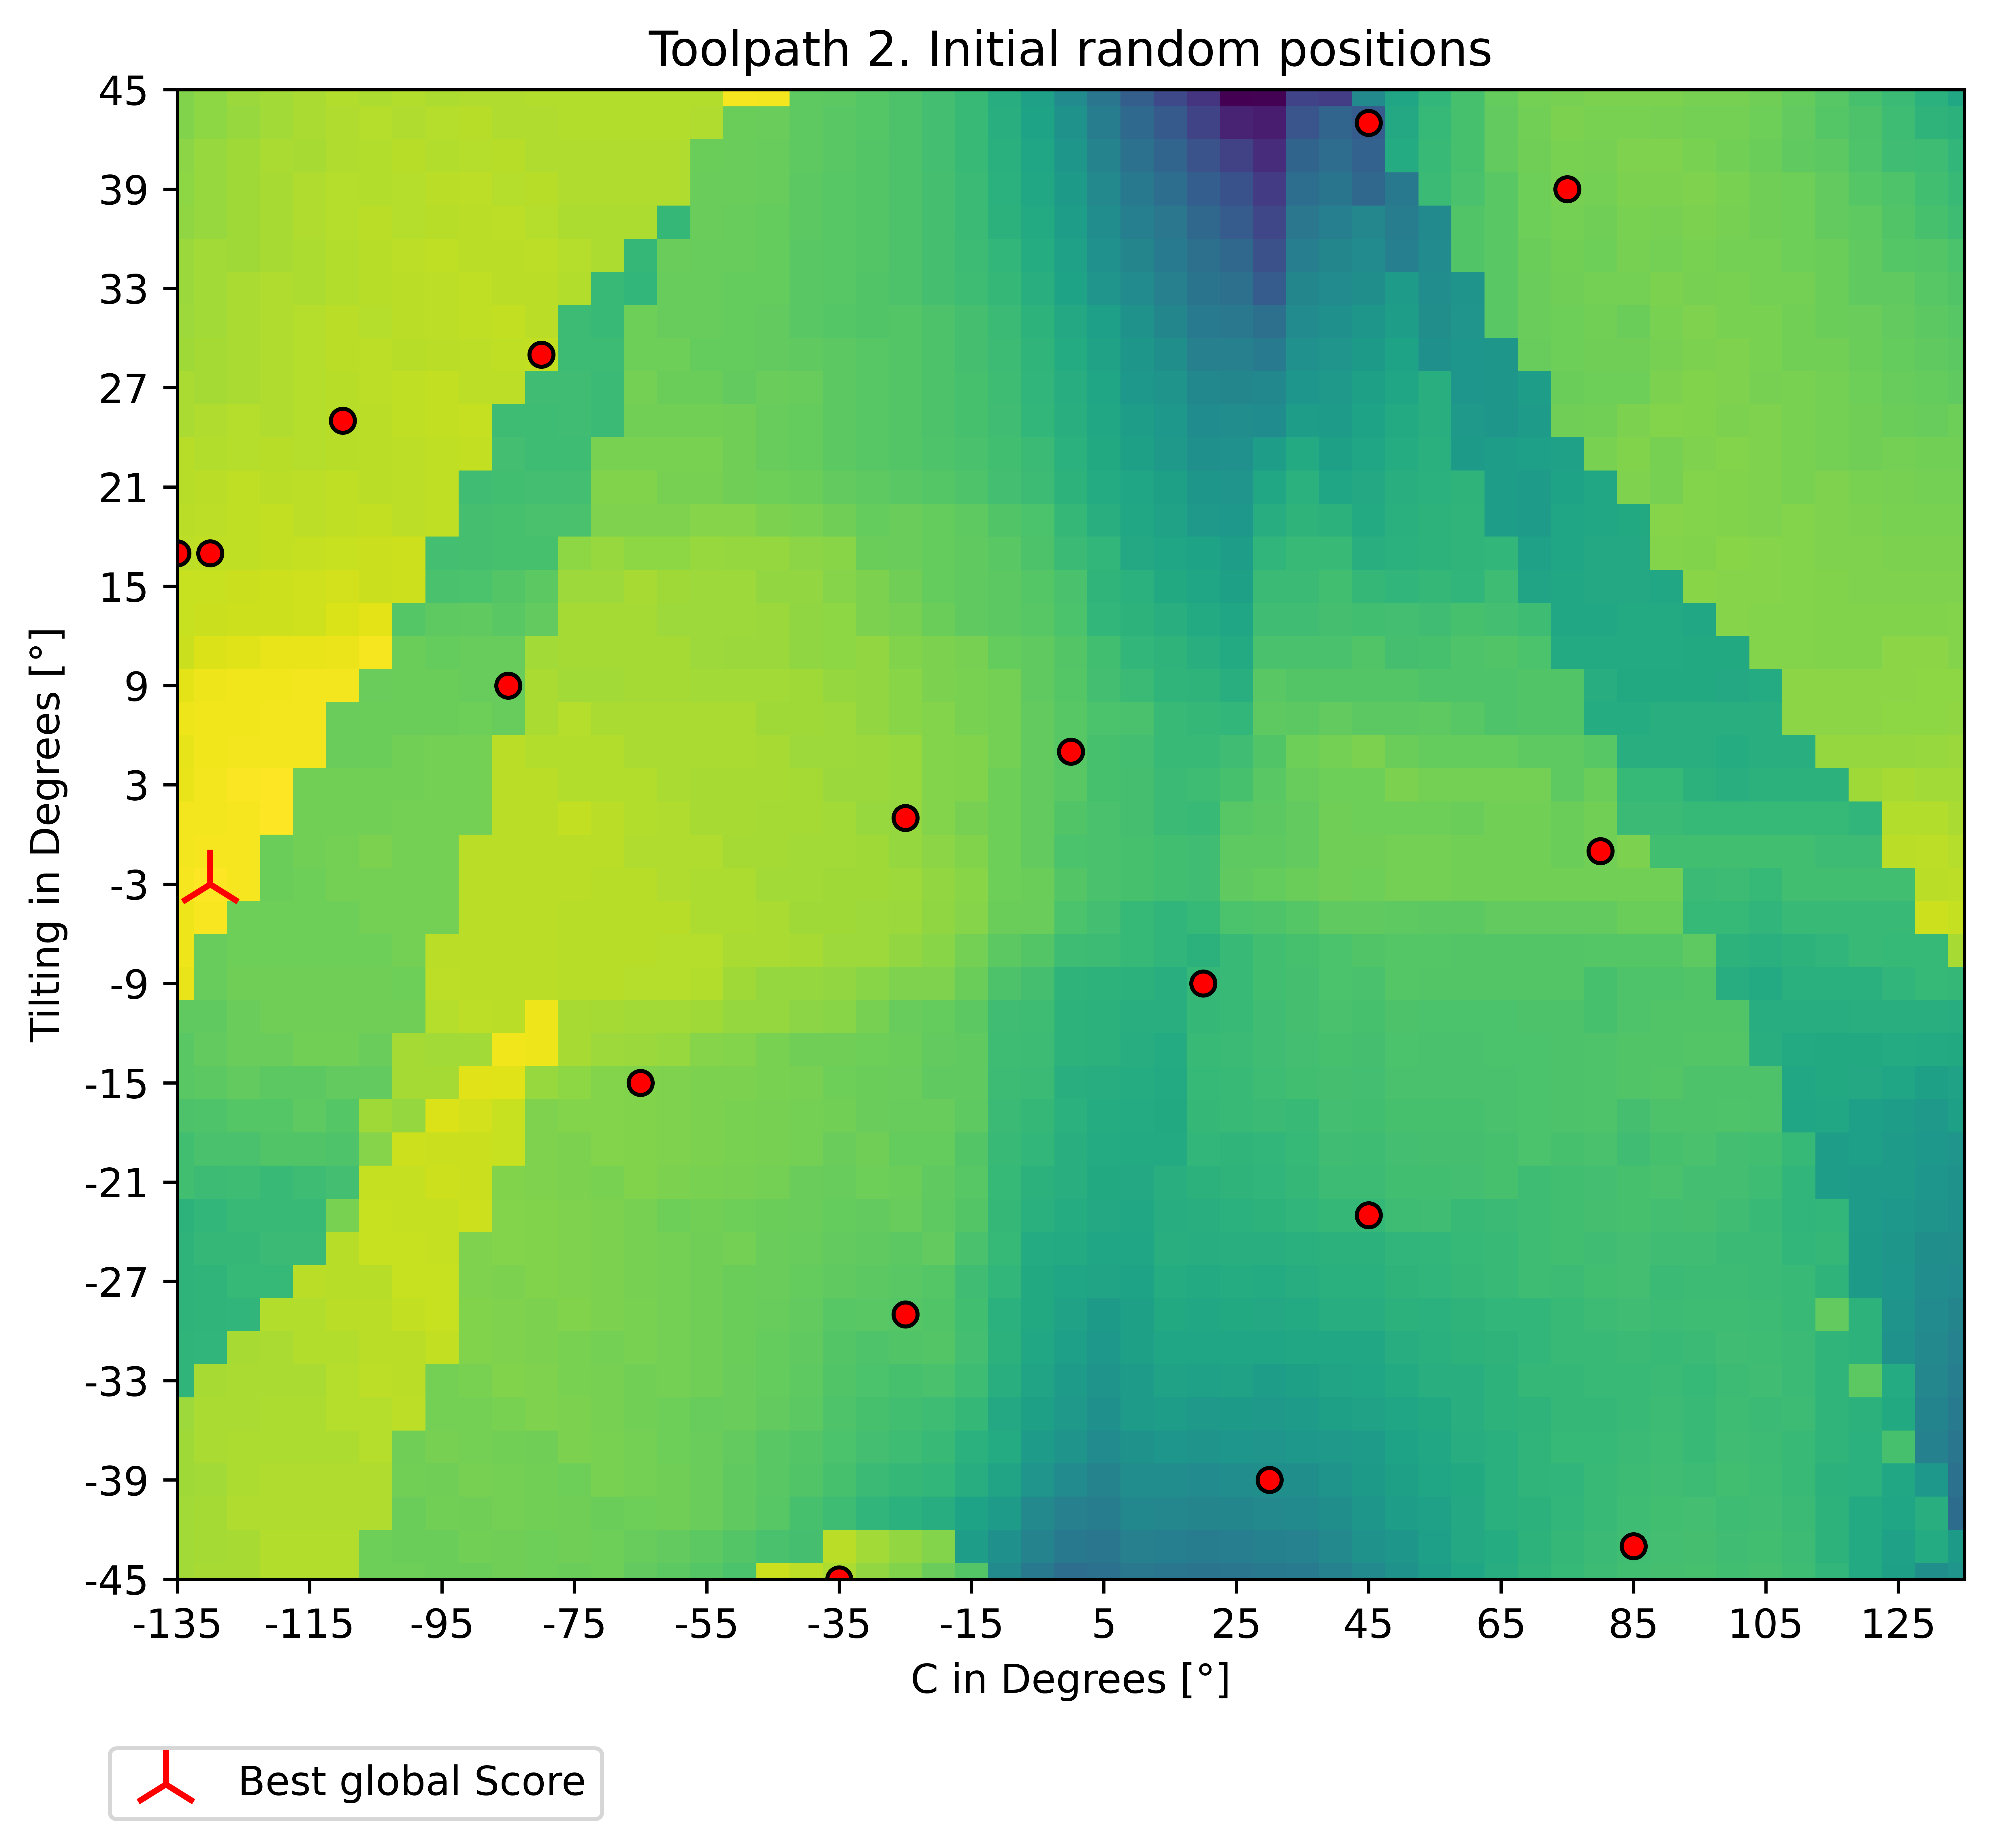
\includegraphics[width=\textwidth]{figures/swarm_true/2_0.png}
		\caption{PSO Initial position toolpath 2}
		\label{tp2_0}
	\end{minipage}\hfill
	\begin{minipage}{0.5\textwidth}
		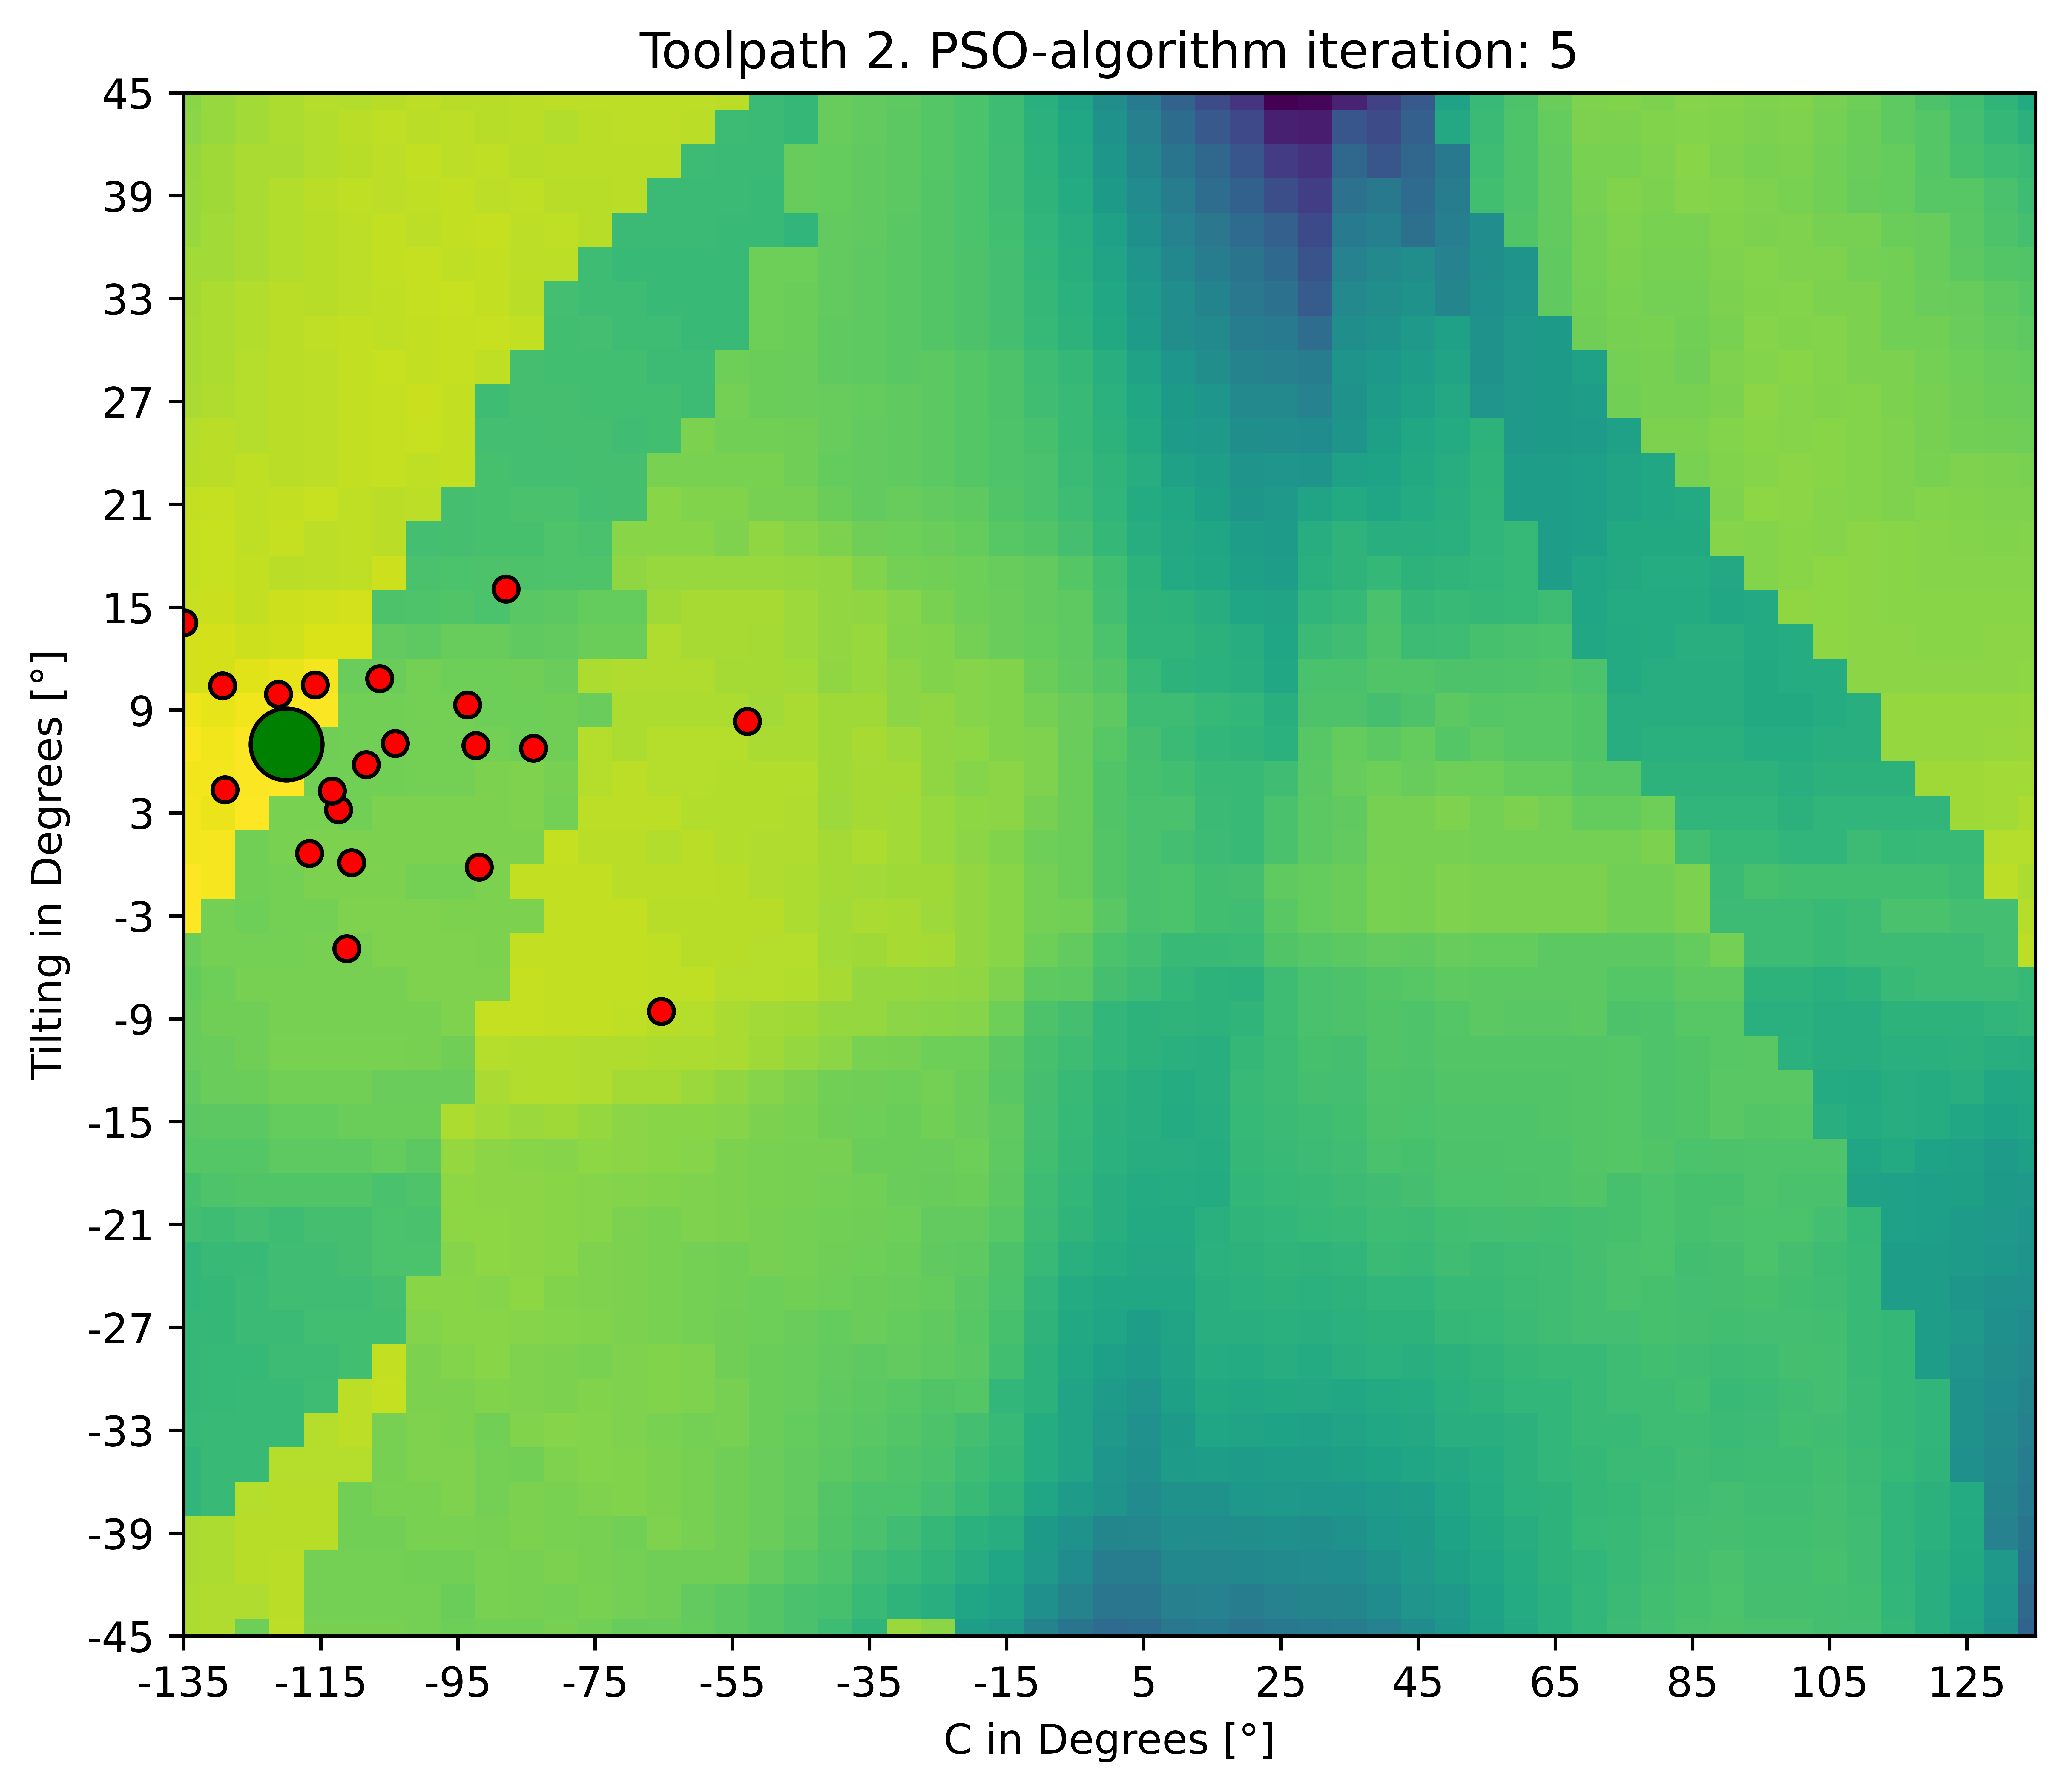
\includegraphics[width=\textwidth]{figures/swarm_true/2_5.png}
		\caption{PSO Iteration 5 on toolpath 2}
		\label{tp2_5}
	\end{minipage}\par
\end{figure}

\newpage
\section{Analysis and Discussion of the Results}%

\subsection{Analysis of the Results}
When analyzing only one redundant degree of freedom, specifically the rotation around the Z-axis, it is clear that there is an improvement in the acceleration in joint 1 and the total combined travel with a increasing negative rotation. This improvement is observed in all three toolpaths. However, it is important to note that the local score of the direction changes is not as smooth as the other analyzed parameters. This is because this value, due to its physical nature, cannot be continuous.

When examining the global score, it becomes evident that finding the global optimum can be challenging. This is because multiple local minima are present. Additionally, the selected process parameters can further contribute to the irregularity of the global score curve.
Depending on the selected process parameters and their importance factor, this process can either turn out a easy or very complicated.

In toolpath 1, the optimal boundary condition is determined as the maximum negative rotation around the Z-axis. This suggests that it may be possible to find an even better boundary condition.
It is worth mentioning that the analysis of each toolpath takes approximately 30 minutes.


When considering the scenario where two degrees of freedom can be set, it is observed that toolpath 1 and toolpath 2 have very similar boundary conditions for the global optimum. This suggests that these two toolpaths do not differ significantly from each other when considering the process parameters alone.

In the case of toolpath 2 with two redundant degrees of freedom, distinct streaks can be observed originating from a positive rotation of 45 degrees of the tilt table.
On the other hand, toolpath 1 exhibits a mostly flat area with a distinct trough. Such a scenario is optimal for a \acrshort{PSO} algorithm.
It is important to note that the calculation of each individual global score matrix takes approximately 50 minutes. 



Based on the results obtained from the \acrshort{PSO} algorithm, it can be concluded that achieving a close-to-optimal result is feasible when the global score matrix yields smooth surfaces. By implementing this approach, a significant reduction in computation time is possible. Instead of calculating the entire matrix, only 100 toolpaths need to be computed using the inverse kinematics algorithm, resulting in a computation time of just 15 minutes.

The number of particles is selected to be as high as possible while also considering the computational costs. Rather than increasing the number of particles, the number of iterations is set to 5 in order to facilitate convergence towards the global optima.
The results clearly show that such a convergence is possible.


NO \acrshort{CAM} EXPLAIN


WAS MUSS NOCH GEMACHR WERDEN DASSS ES Auf echtem Gcode und \acrshort{CAM} läuft ???




\newpage
\subsection{Discussion of the Results}%
Even though the results show a very promising outcome, it is necessary to consider some additional factors. One of the most obvious elements is that only three very simple toolpaths are analyzed. To validate this method in detail, it is necessary to use real-life production G-code with correctly modeled robotic systems and analyze whether it can be optimized. One of the possible limiting factors is that the rotation values for A and B are always set to 0 in the toolpaths' coordinate system. It should be noted that this work only provides a limited excerpt and does not analyze complex multi-axis operations, which are a significant advantage and building block of the \acrshort{WAAM} process.

The selected inverse kinematics algorithm is not designed for optimal high-performance calculations, making it infeasible to use when dealing with toolpaths that have millions of points. Additionally, the algorithm calculates the joint position numerically rather than analytically, which can result in unexpected robot poses. \acrshort{CAM} software such as \textit{Siemens NX} offers additional options for inverse kinematics that can be used to fine-tune the behavior of the robot.

When analyzing multiple process parameters, it is not guaranteed that the resulting surface will be smooth and optimal for the selected optimization algorithm. Additionally, when working with a \acrshort{PSO} algorithm, the final result strongly depends on the initial distribution of the particles. If the optimum is a very tight and sharp spike, the probability of finding the optimal boundary condition is significantly lower. This is particularly true in systems with 3 or more redundant degrees of freedom, where simple optimization algorithms can lead to suboptimal results or require unfeasibly long computation times.

In general, the presented methodology does provide a solid basis as a proof of concept for the proposed method. However, additional implementations are necessary for it to be feasible in an industrial environment.
